\documentclass[12pt]{extarticle}
\usepackage[paperwidth=18in,paperheight=7.5in]{geometry}
\usepackage{amsmath}
\usepackage{hyperref}
\usepackage{multirow}
\usepackage{pdfpages}
\usepackage[utf8]{inputenc}
\title{Kaon mixing: chiral and continuum extrapolations}
\author{R Mukherjee}
\date{\today}
\begin{document}
\maketitle
\tableofcontents
\clearpage
\begin{figure}
\centering
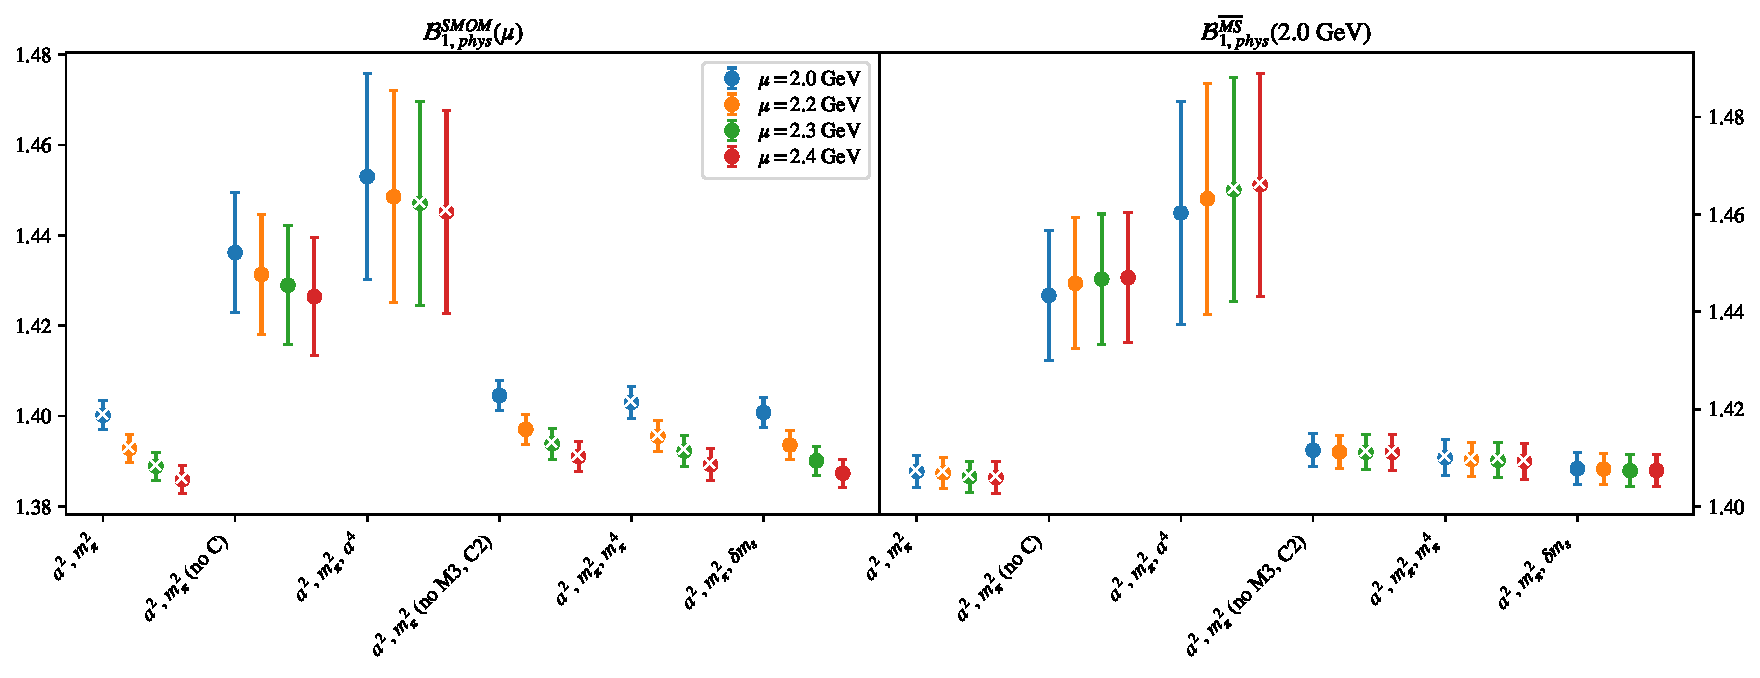
\includegraphics[page=1, width=1.1\textwidth]{VVpAA/NPR/fit_summary_bag.pdf}
\caption{$\mathcal{B}_{1}$\\(left) $\mathcal{B}_{phys}$ in RI/SMOM scheme from fit variations (fits with $p$-value $<0.05$ marked with ``$\times$"). \\(right) $\mathcal{B}_{phys}$ in $\overline{MS}$ computed using $\mathcal{B}^{\overline{MS}} = R^{\overline{MS}\leftarrow SMOM}(2.0)\sigma_{npt}(2.0,\mu) \mathcal{B}^{SMOM}(\mu)$.}
\end{figure}
\clearpage
\begin{figure}
\centering
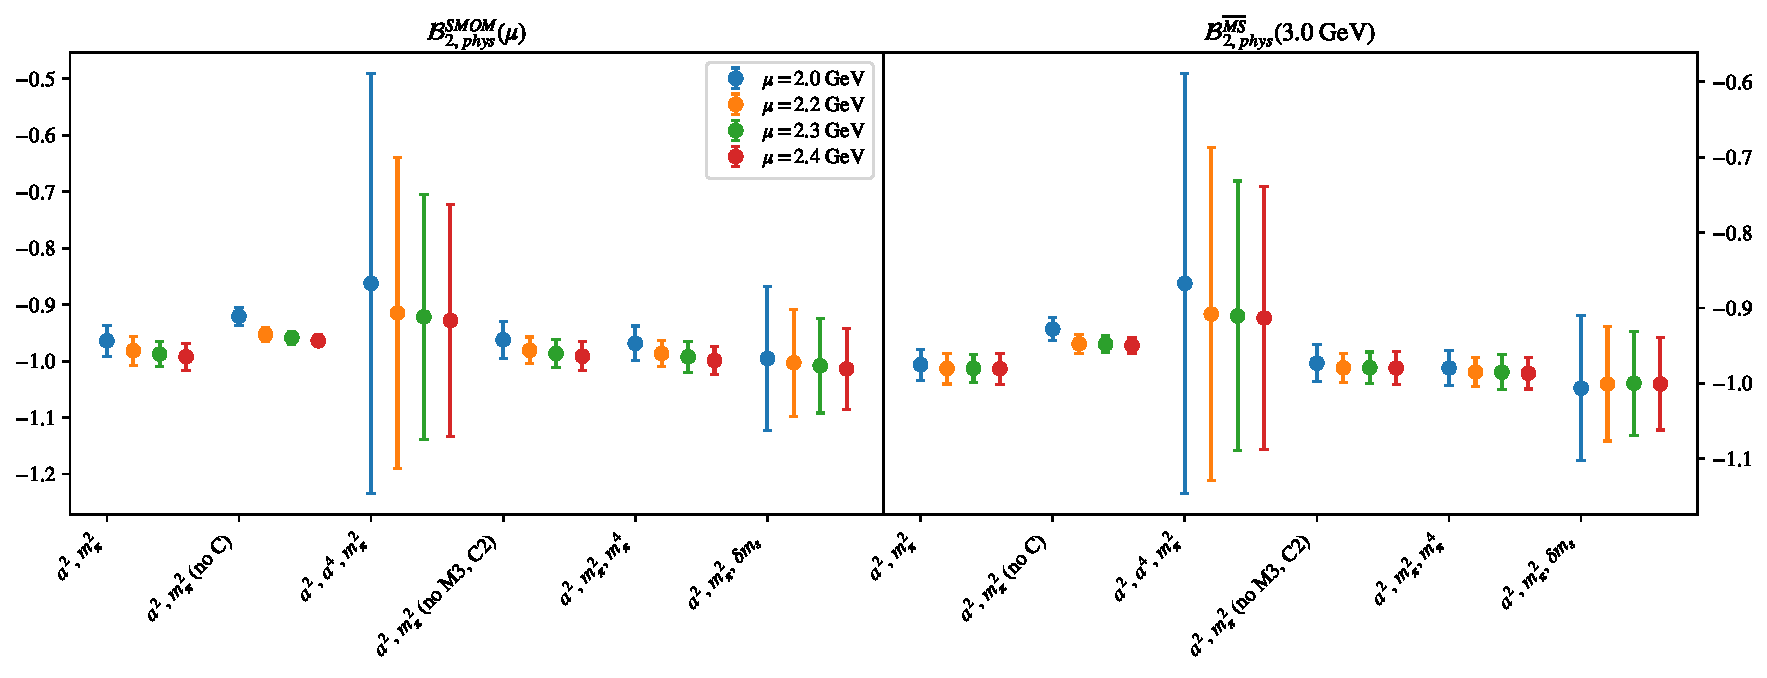
\includegraphics[page=1, width=1.1\textwidth]{VVmAA/NPR/fit_summary_bag.pdf}
\caption{$\mathcal{B}_{2}$\\(left) $\mathcal{B}_{phys}$ in RI/SMOM scheme from fit variations (fits with $p$-value $<0.05$ marked with ``$\times$"). \\(right) $\mathcal{B}_{phys}$ in $\overline{MS}$ computed using $\mathcal{B}^{\overline{MS}} = R^{\overline{MS}\leftarrow SMOM}(3.0)\sigma_{npt}(3.0,\mu) \mathcal{B}^{SMOM}(\mu)$.}
\end{figure}
\clearpage
\begin{figure}
\centering
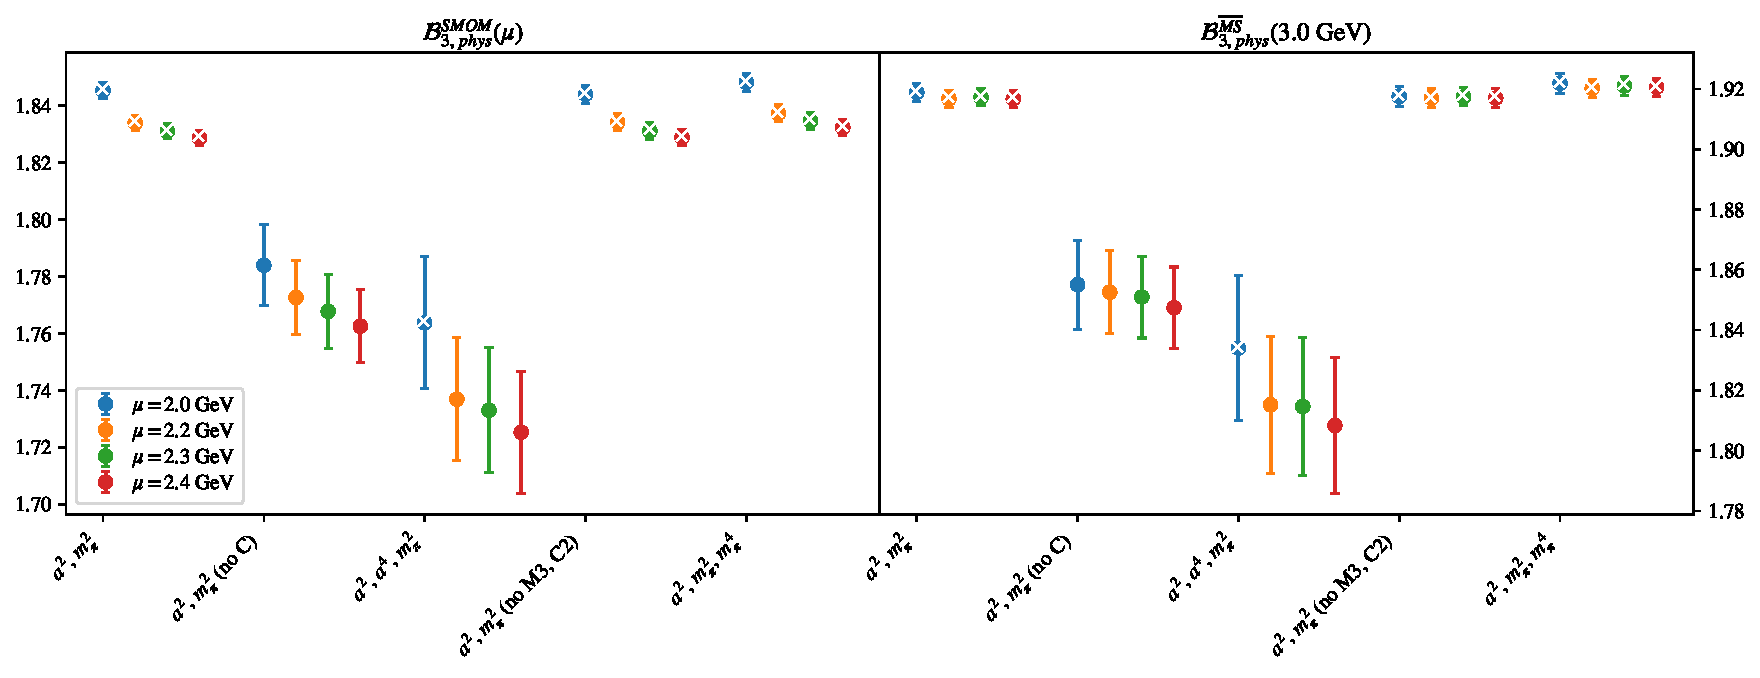
\includegraphics[page=1, width=1.1\textwidth]{SSmPP/NPR/fit_summary_bag.pdf}
\caption{$\mathcal{B}_{3}$\\(left) $\mathcal{B}_{phys}$ in RI/SMOM scheme from fit variations (fits with $p$-value $<0.05$ marked with ``$\times$"). \\(right) $\mathcal{B}_{phys}$ in $\overline{MS}$ computed using $\mathcal{B}^{\overline{MS}} = R^{\overline{MS}\leftarrow SMOM}(3.0)\sigma_{npt}(3.0,\mu) \mathcal{B}^{SMOM}(\mu)$.}
\end{figure}
\clearpage
\begin{figure}
\centering
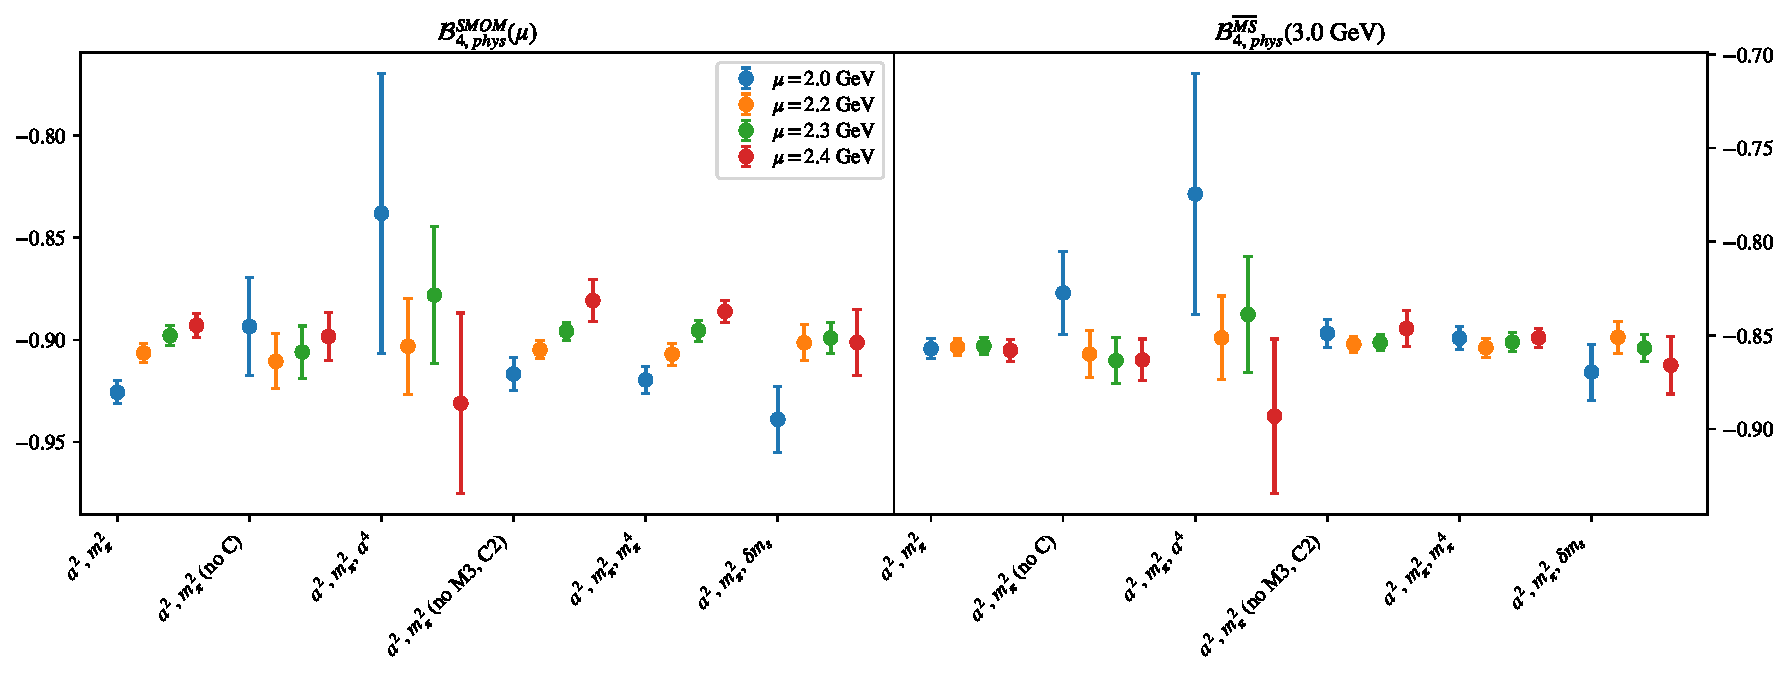
\includegraphics[page=1, width=1.1\textwidth]{SSpPP/NPR/fit_summary_bag.pdf}
\caption{$\mathcal{B}_{4}$\\(left) $\mathcal{B}_{phys}$ in RI/SMOM scheme from fit variations (fits with $p$-value $<0.05$ marked with ``$\times$"). \\(right) $\mathcal{B}_{phys}$ in $\overline{MS}$ computed using $\mathcal{B}^{\overline{MS}} = R^{\overline{MS}\leftarrow SMOM}(3.0)\sigma_{npt}(3.0,\mu) \mathcal{B}^{SMOM}(\mu)$.}
\end{figure}
\clearpage
\begin{figure}
\centering
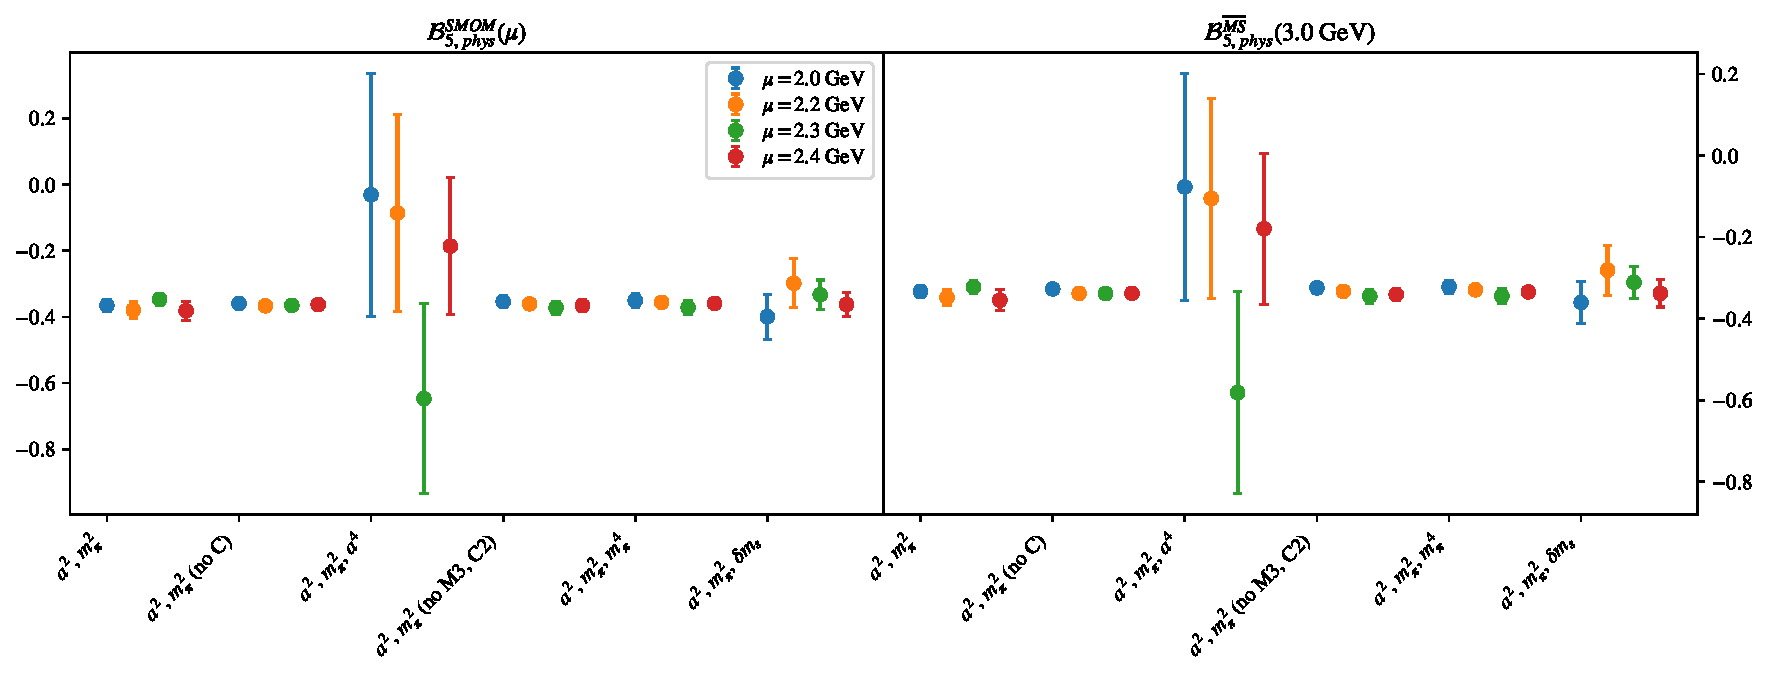
\includegraphics[page=1, width=1.1\textwidth]{TT/NPR/fit_summary_bag.pdf}
\caption{$\mathcal{B}_{5}$\\(left) $\mathcal{B}_{phys}$ in RI/SMOM scheme from fit variations (fits with $p$-value $<0.05$ marked with ``$\times$"). \\(right) $\mathcal{B}_{phys}$ in $\overline{MS}$ computed using $\mathcal{B}^{\overline{MS}} = R^{\overline{MS}\leftarrow SMOM}(3.0)\sigma_{npt}(3.0,\mu) \mathcal{B}^{SMOM}(\mu)$.}
\end{figure}
\clearpage
\section{$\mathcal{B}_1$}
\begin{table}[h!]
\begin{center}
\begin{tabular}{|c|c|c|c|c|c|c|}
\hline
$\mu$ (GeV) & $a^2$, $m_\pi^2$& $a^2$, $m_\pi^2$ (no C)& $a^2$, $a^4$, $m_\pi^2$& $a^2$, $m_\pi^2$ (no M3, C2)& $a^2$, $m_\pi^2$, $m_\pi^4$& $a^2$, $m_\pi^2$, $\delta m_s$\\
\hline
2.0& \hyperlink{VVpAA/NPR/a2m2_20.pdf.1}{\textbf{1.4024(27)}: 2.267 (0.045)} & \hyperlink{VVpAA/NPR/a2m2noC_20.pdf.1}{\textbf{1.415(12)}: 0.844 (0.43)} & \hyperlink{VVpAA/NPR/a2a4m2_20.pdf.1}{\textbf{1.415(21)}: 2.736 (0.027)} & \hyperlink{VVpAA/NPR/a2m2mcut_20.pdf.1}{\textbf{1.4081(32)}: 0.218 (0.884)} & \hyperlink{VVpAA/NPR/a2m2m4_20.pdf.1}{\textbf{1.4081(33)}: 0.97 (0.423)} & \hyperlink{VVpAA/NPR/a2m2delm_20.pdf.1}{\textbf{1.3999(34)}: 2.367 (0.05)}\\
2.2& \hyperlink{VVpAA/NPR/a2m2_22.pdf.1}{\textbf{1.3950(27)}: 2.615 (0.023)} & \hyperlink{VVpAA/NPR/a2m2noC_22.pdf.1}{\textbf{1.410(12)}: 0.984 (0.374)} & \hyperlink{VVpAA/NPR/a2a4m2_22.pdf.1}{\textbf{1.412(21)}: 3.092 (0.015)} & \hyperlink{VVpAA/NPR/a2m2mcut_22.pdf.1}{\textbf{1.4011(32)}: 0.358 (0.783)} & \hyperlink{VVpAA/NPR/a2m2m4_22.pdf.1}{\textbf{1.4010(33)}: 1.224 (0.298)} & \hyperlink{VVpAA/NPR/a2m2delm_22.pdf.1}{\textbf{1.3921(34)}: 2.594 (0.035)}\\
2.3& \hyperlink{VVpAA/NPR/a2m2_23.pdf.1}{\textbf{1.3916(27)}: 2.84 (0.014)} & \hyperlink{VVpAA/NPR/a2m2noC_23.pdf.1}{\textbf{1.408(12)}: 1.059 (0.347)} & \hyperlink{VVpAA/NPR/a2a4m2_23.pdf.1}{\textbf{1.411(21)}: 3.329 (0.01)} & \hyperlink{VVpAA/NPR/a2m2mcut_23.pdf.1}{\textbf{1.3979(32)}: 0.45 (0.717)} & \hyperlink{VVpAA/NPR/a2m2m4_23.pdf.1}{\textbf{1.3977(33)}: 1.403 (0.23)} & \hyperlink{VVpAA/NPR/a2m2delm_23.pdf.1}{\textbf{1.3885(33)}: 2.747 (0.027)}\\
2.4& \hyperlink{VVpAA/NPR/a2m2_24.pdf.1}{\textbf{1.3887(26)}: 2.947 (0.012)} & \hyperlink{VVpAA/NPR/a2m2noC_24.pdf.1}{\textbf{1.406(12)}: 1.112 (0.329)} & \hyperlink{VVpAA/NPR/a2a4m2_24.pdf.1}{\textbf{1.408(21)}: 3.451 (0.008)} & \hyperlink{VVpAA/NPR/a2m2mcut_24.pdf.1}{\textbf{1.3952(32)}: 0.472 (0.702)} & \hyperlink{VVpAA/NPR/a2m2m4_24.pdf.1}{\textbf{1.3949(32)}: 1.459 (0.212)} & \hyperlink{VVpAA/NPR/a2m2delm_24.pdf.1}{\textbf{1.3855(33)}: 2.832 (0.023)}\\
\hline
\end{tabular}
\caption{Physical point value from chiral and continuum extrapolation at renormalisation scale $\mu$. Entries are \textbf{value(error)}: $\chi^2/\text{DOF}$ ($p$-value).}
\end{center}
\end{table}
\begin{table}[h!]
\begin{center}
\begin{tabular}{|c c|c|c|c|c|c|c|}
\hline
$\mu$ (GeV) &  & $a^2$, $m_\pi^2$& $a^2$, $m_\pi^2$ (no C)& $a^2$, $a^4$, $m_\pi^2$& $a^2$, $m_\pi^2$ (no M3, C2)& $a^2$, $m_\pi^2$, $m_\pi^4$& $a^2$, $m_\pi^2$, $\delta m_s$\\
\hline
\multirow{2}{0.5in}{2.0} & $\alpha$ & 0.0975(73)& 0.052(53)& 0.011& 0.0838(83)& 0.0843(83)& 0.1032(88)\\
 & $\beta$ & 0.00288(16)& 0.00231(32)& 0.00289(16)& 0.00206(32)& 0.00034(95)& 0.00296(17)\\
\hline
\multirow{2}{0.5in}{2.2} & $\alpha$ & 0.1015(73)& 0.044(52)& -0.015& 0.0867(84)& 0.0876(83)& 0.1082(87)\\
 & $\beta$ & 0.00282(15)& 0.00222(32)& 0.00284(15)& 0.00196(31)& 0.00019(94)& 0.00292(16)\\
\hline
\multirow{2}{0.5in}{2.3} & $\alpha$ & 0.1033(73)& 0.039(52)& -0.026& 0.0879(84)& 0.0891(83)& 0.1107(87)\\
 & $\beta$ & 0.00280(15)& 0.00218(31)& 0.00283(15)& 0.00192(31)& 0.00011(94)& 0.00291(16)\\
\hline
\multirow{2}{0.5in}{2.4} & $\alpha$ & 0.1041(72)& 0.039(52)& -0.029& 0.0883(84)& 0.0895(83)& 0.1116(86)\\
 & $\beta$ & 0.00279(15)& 0.00216(31)& 0.00282(15)& 0.00190(31)& 0.0& 0.00290(16)\\
\hline
\end{tabular}
\caption{Fit values of coefficients in $Q = Q_{phys} + \mathbf{\alpha} a^2 + \mathbf{\beta}\left(\frac{m_\pi^2}{f_\pi^2}-\frac{m_{\pi,PDG}^2}{f_\pi^2}\right) + \ldots$.}
\end{center}
\end{table}
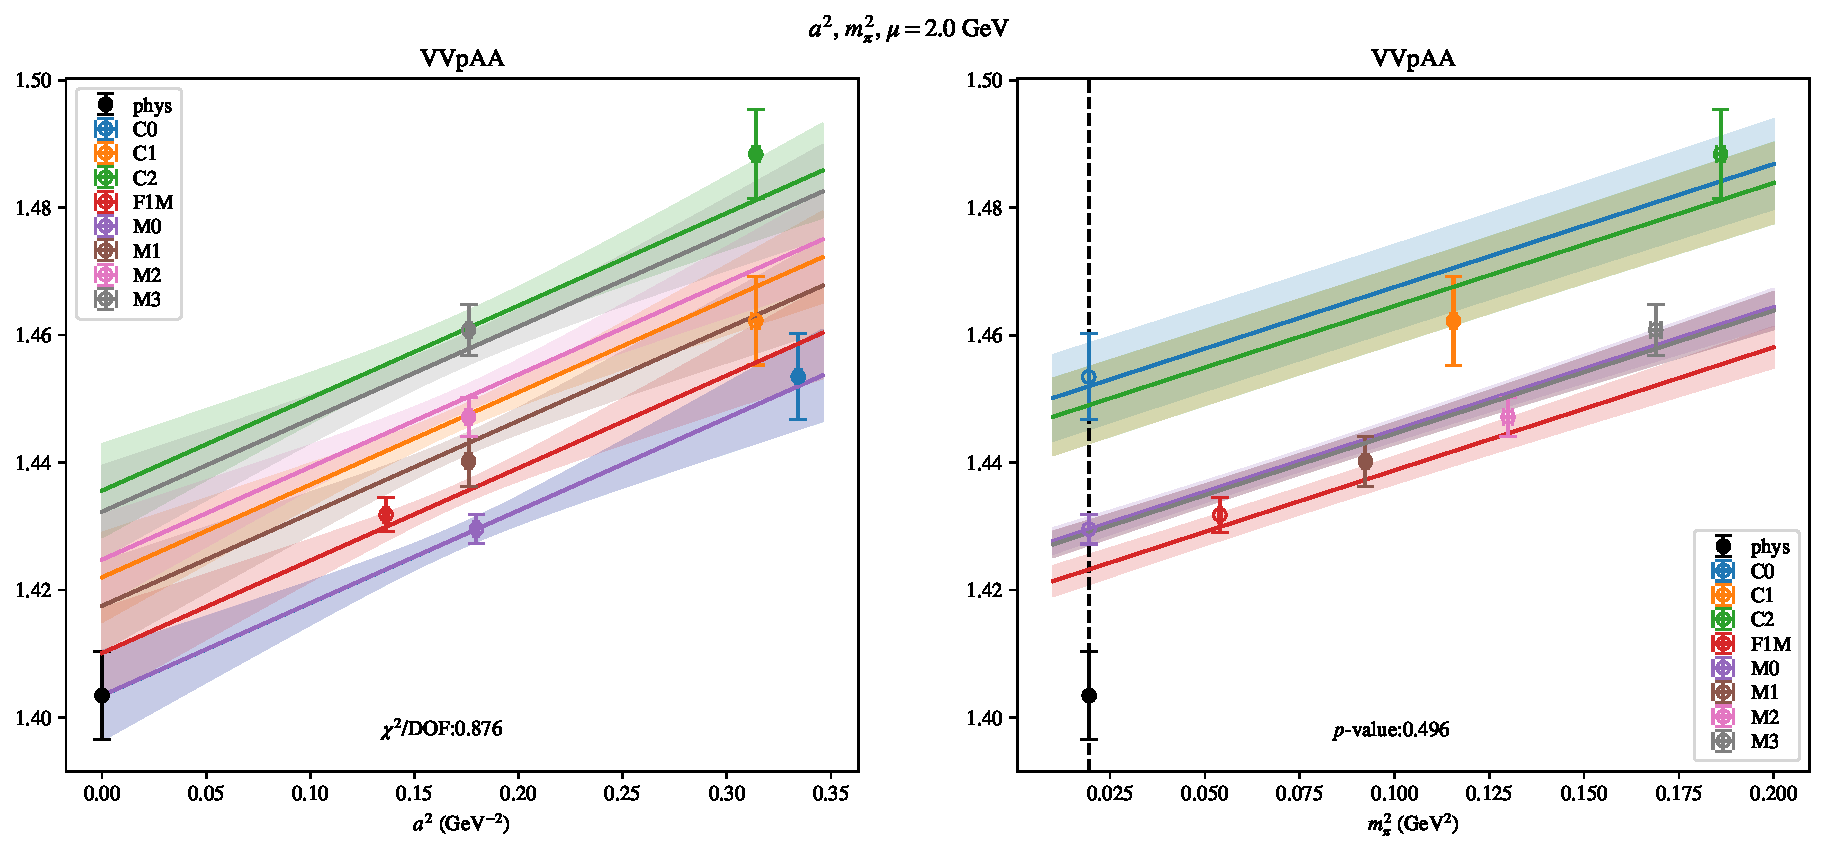
\includepdf[link, pages=-]{VVpAA/NPR/a2m2_20.pdf}
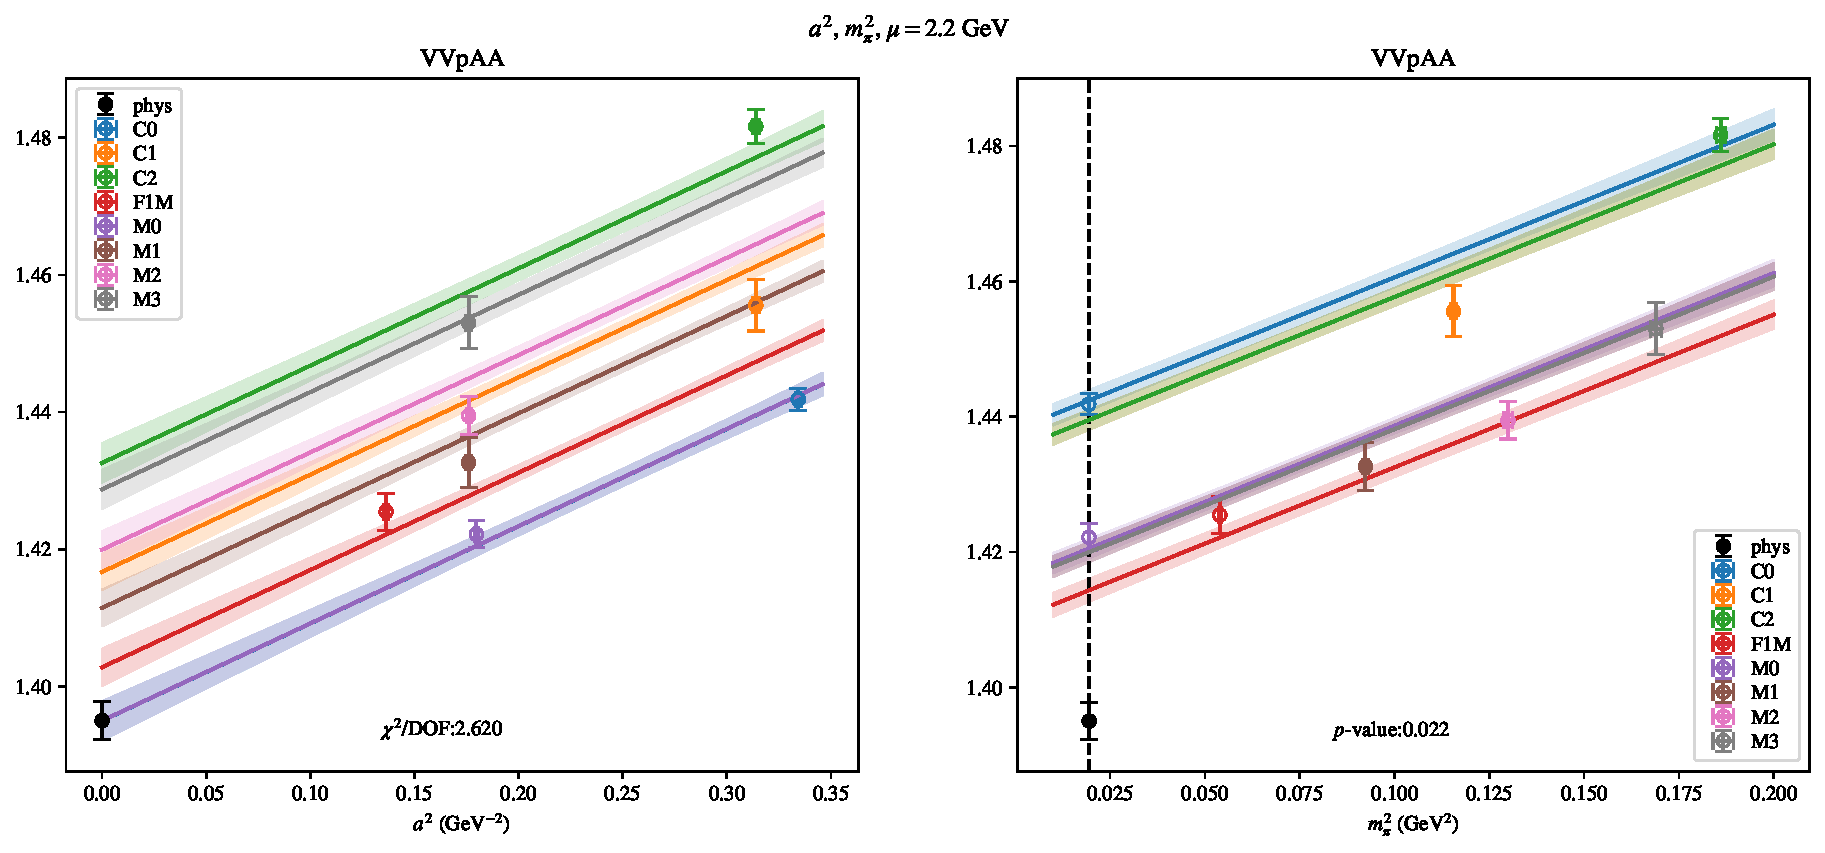
\includepdf[link, pages=-]{VVpAA/NPR/a2m2_22.pdf}
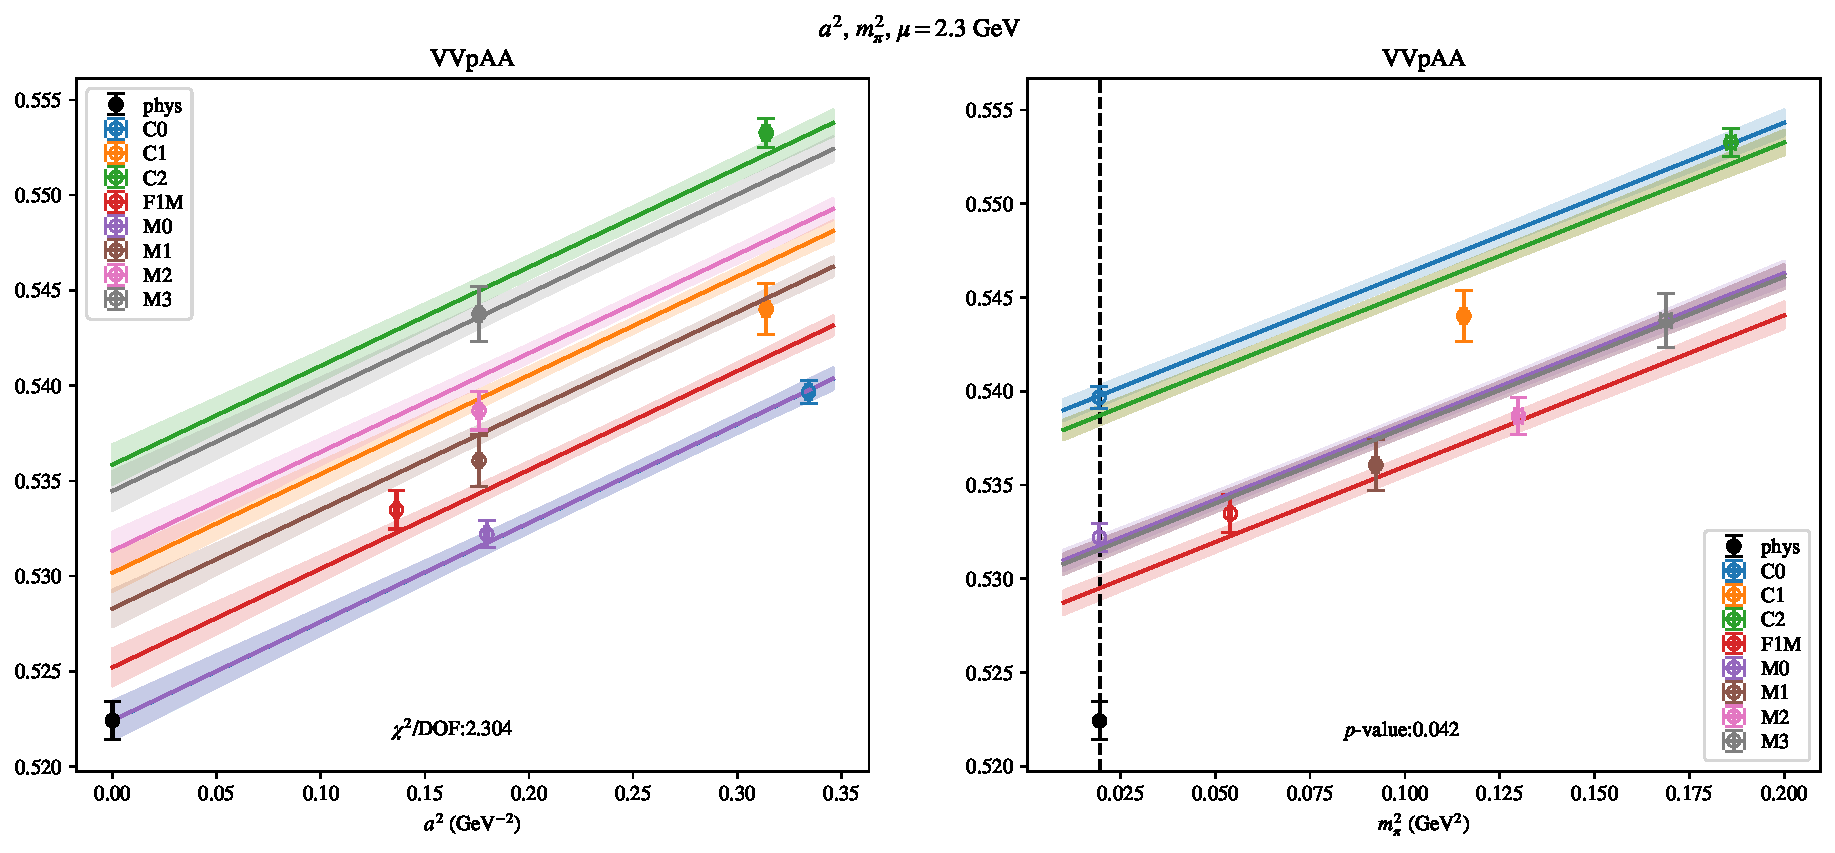
\includepdf[link, pages=-]{VVpAA/NPR/a2m2_23.pdf}
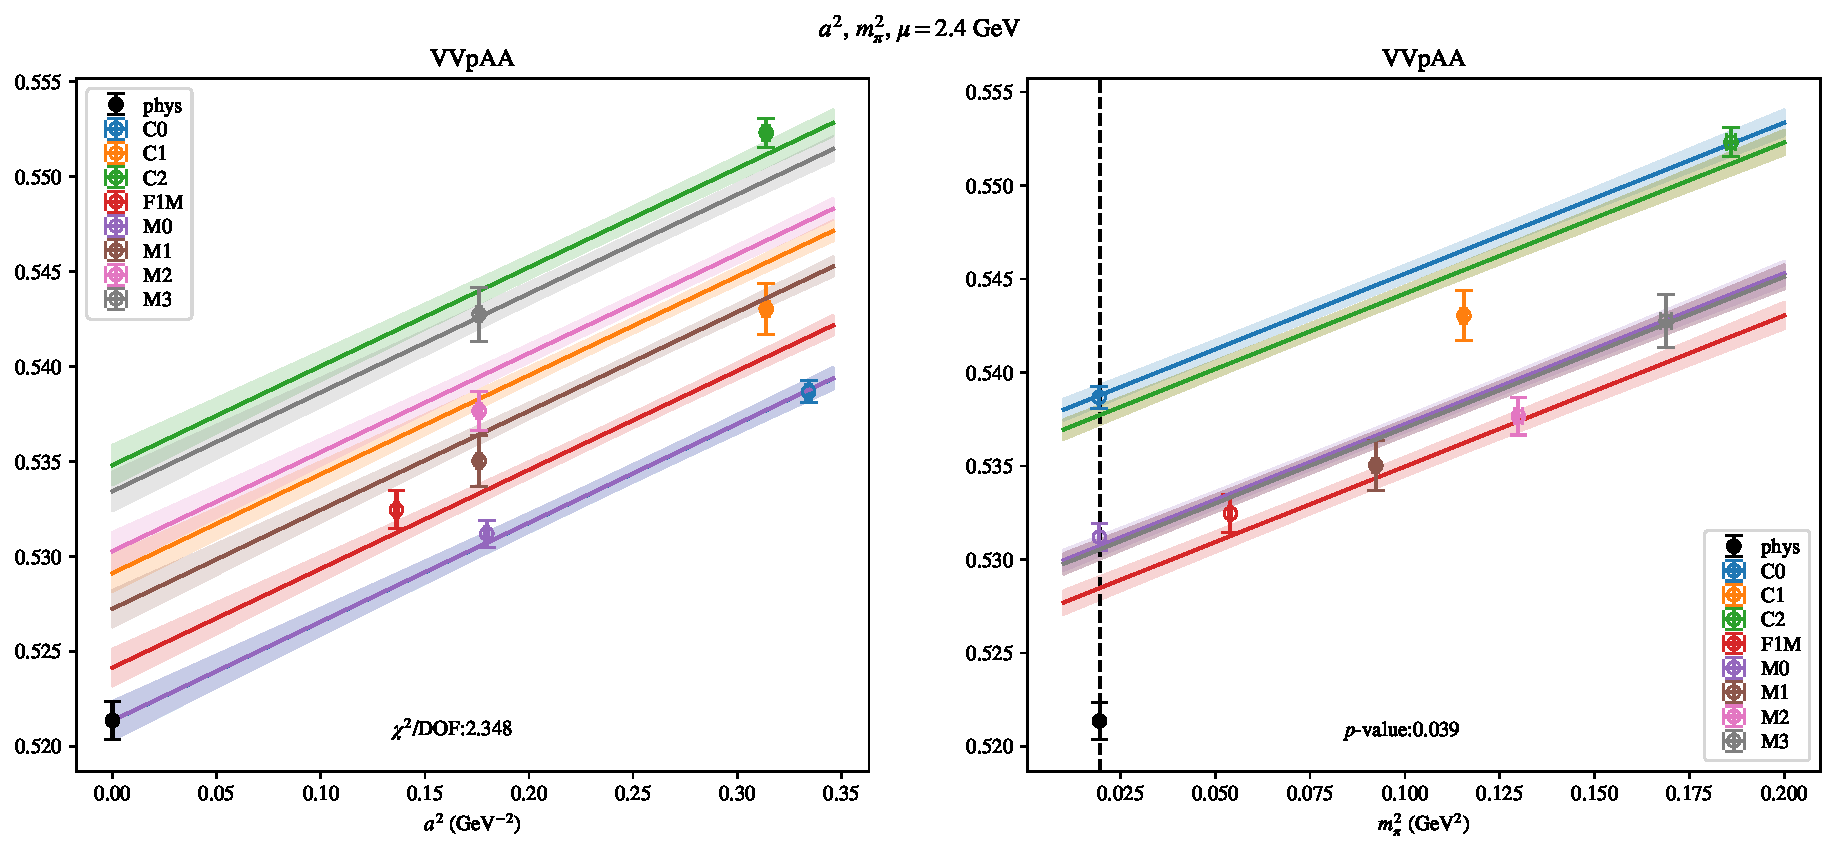
\includepdf[link, pages=-]{VVpAA/NPR/a2m2_24.pdf}
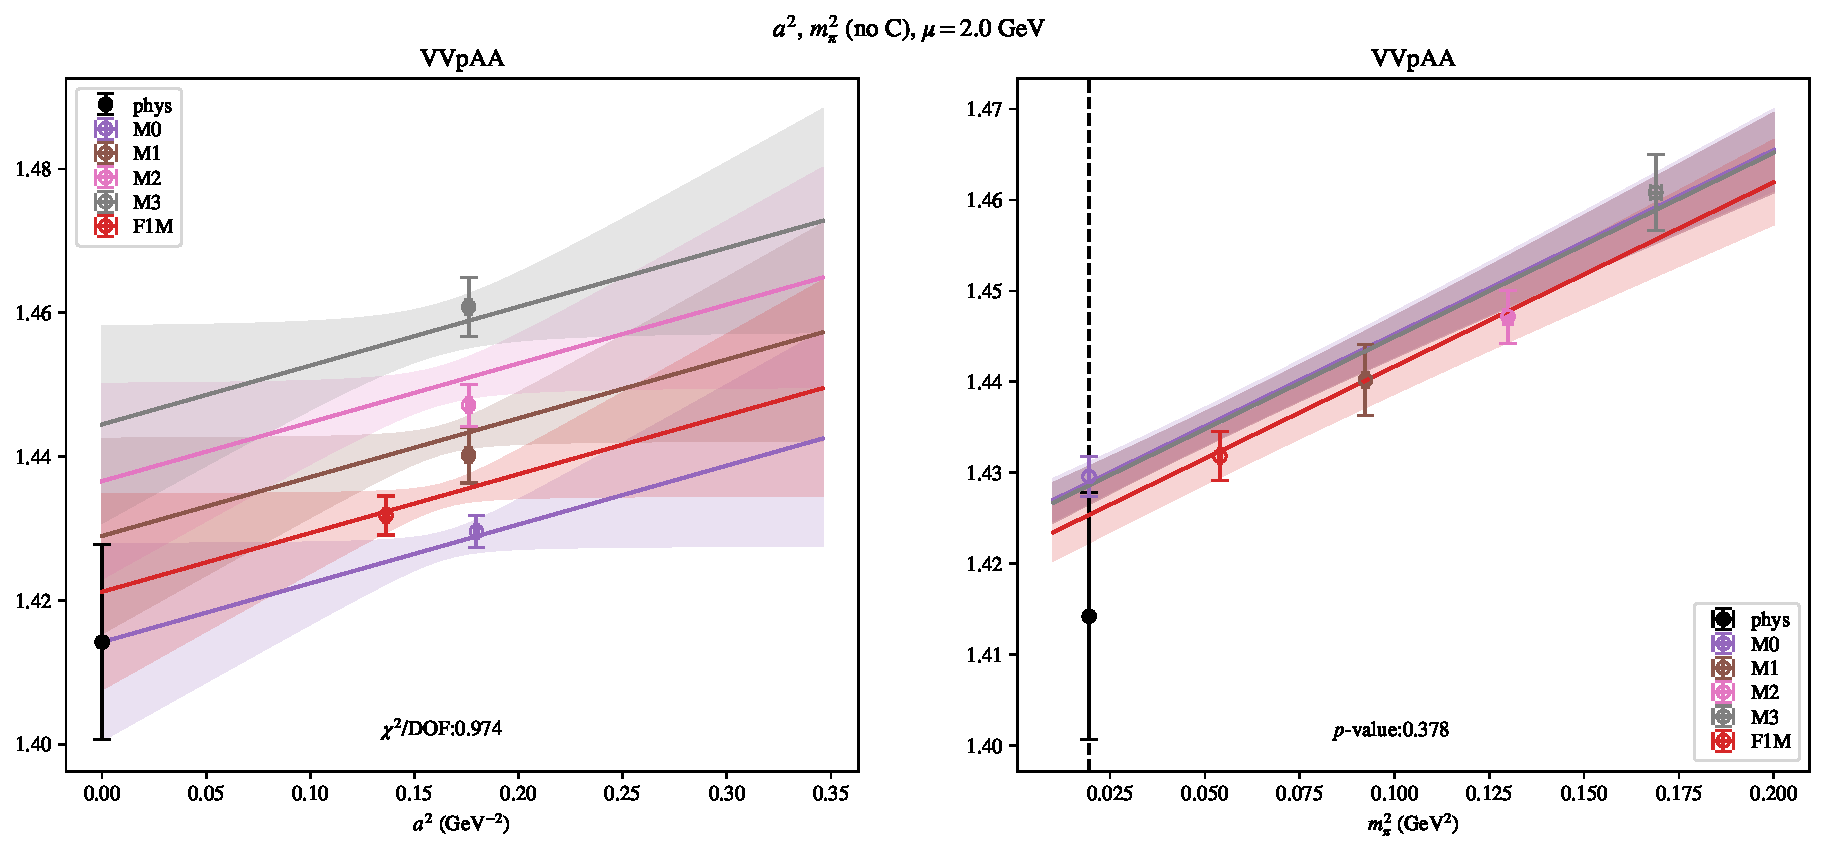
\includepdf[link, pages=-]{VVpAA/NPR/a2m2noC_20.pdf}
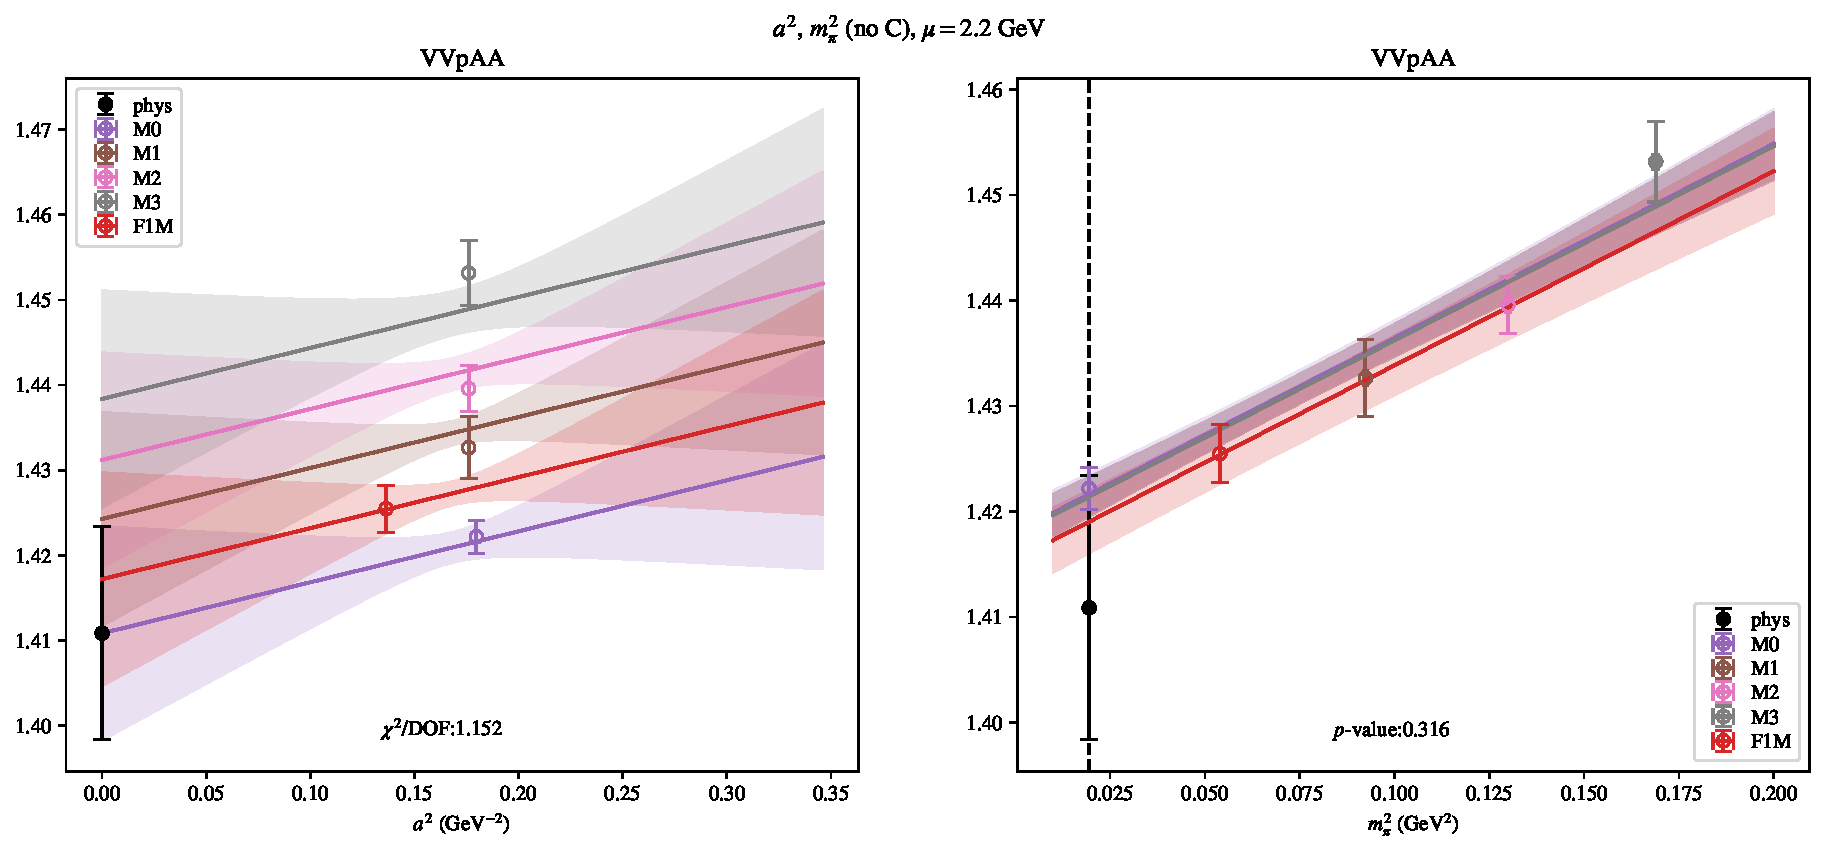
\includepdf[link, pages=-]{VVpAA/NPR/a2m2noC_22.pdf}
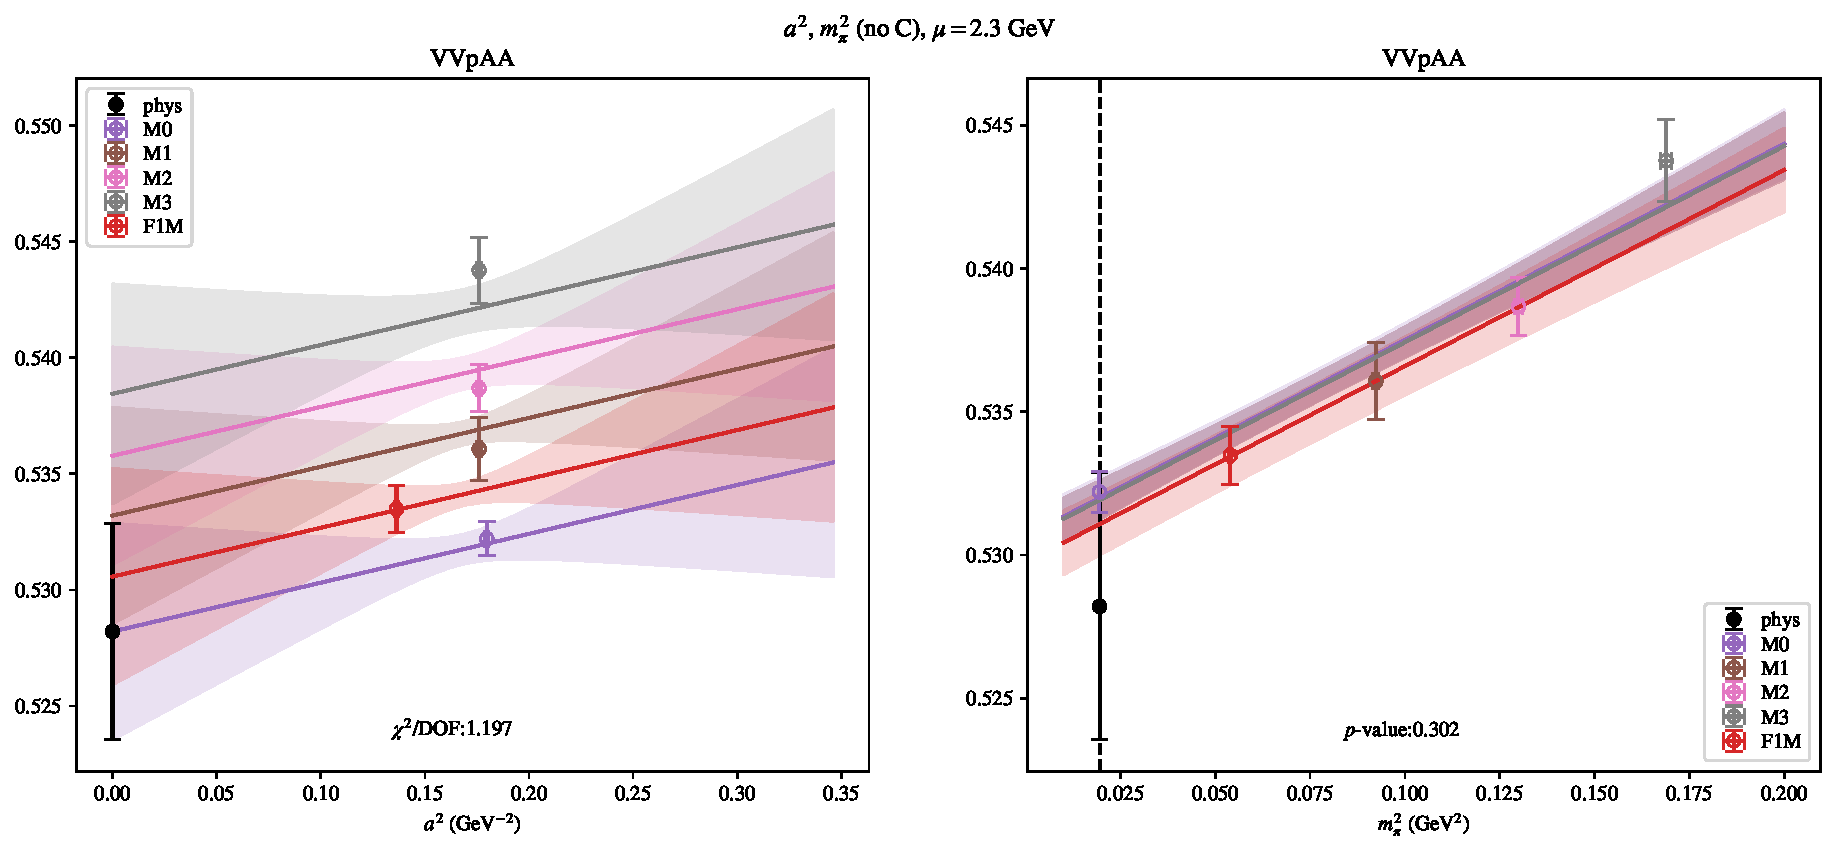
\includepdf[link, pages=-]{VVpAA/NPR/a2m2noC_23.pdf}
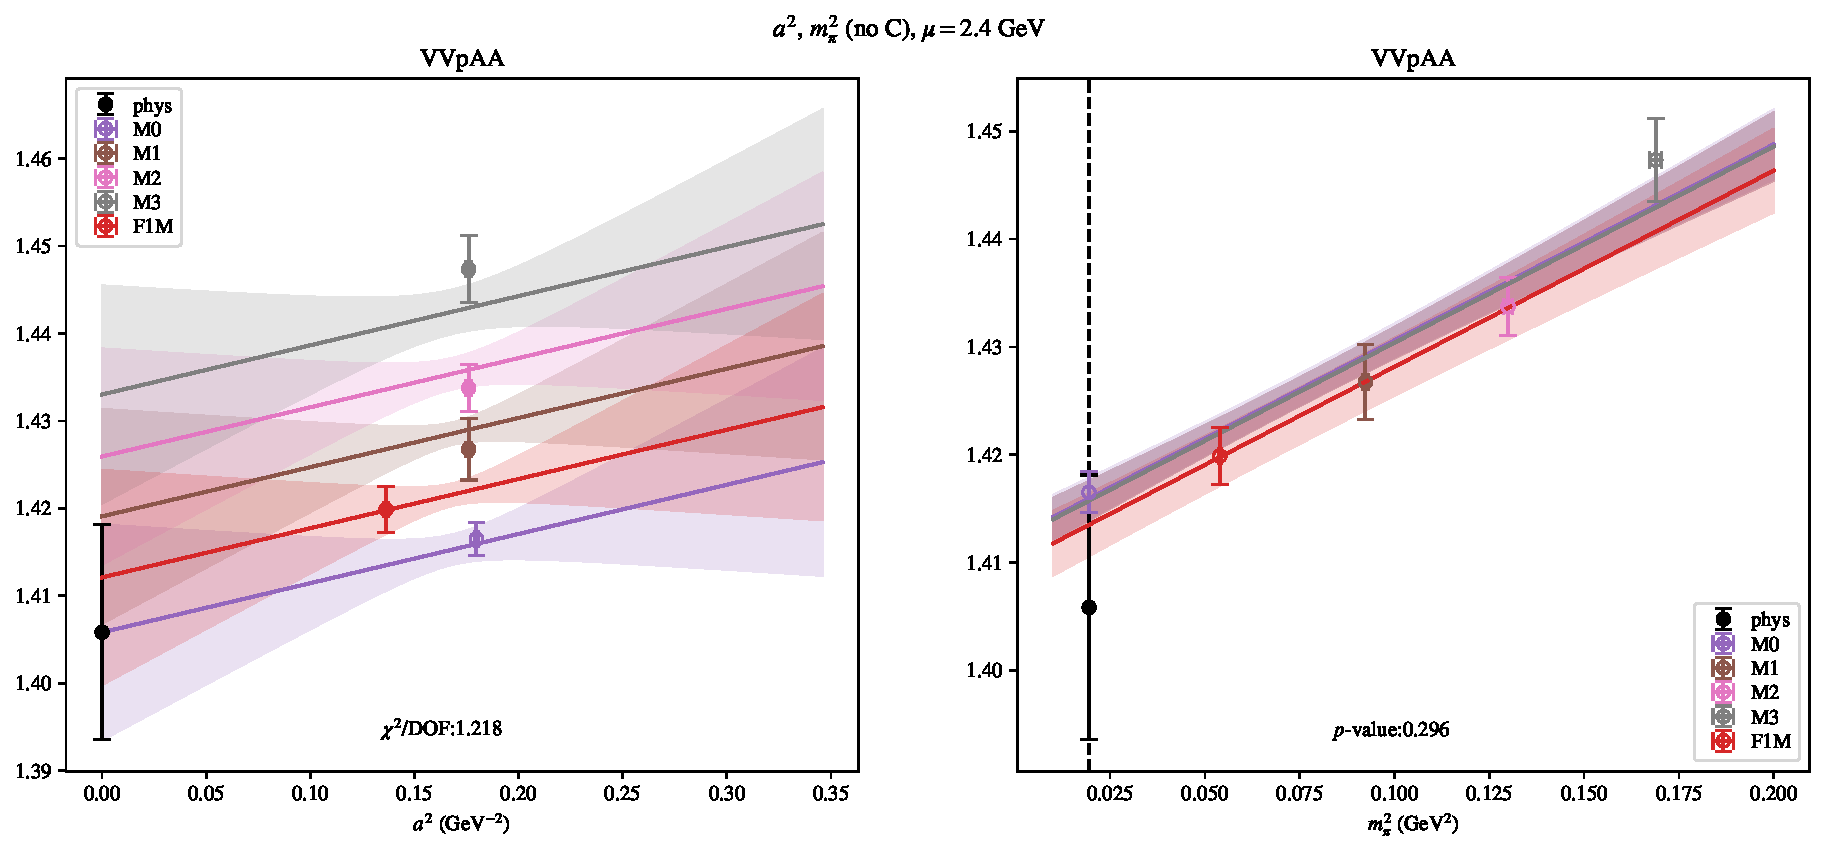
\includepdf[link, pages=-]{VVpAA/NPR/a2m2noC_24.pdf}
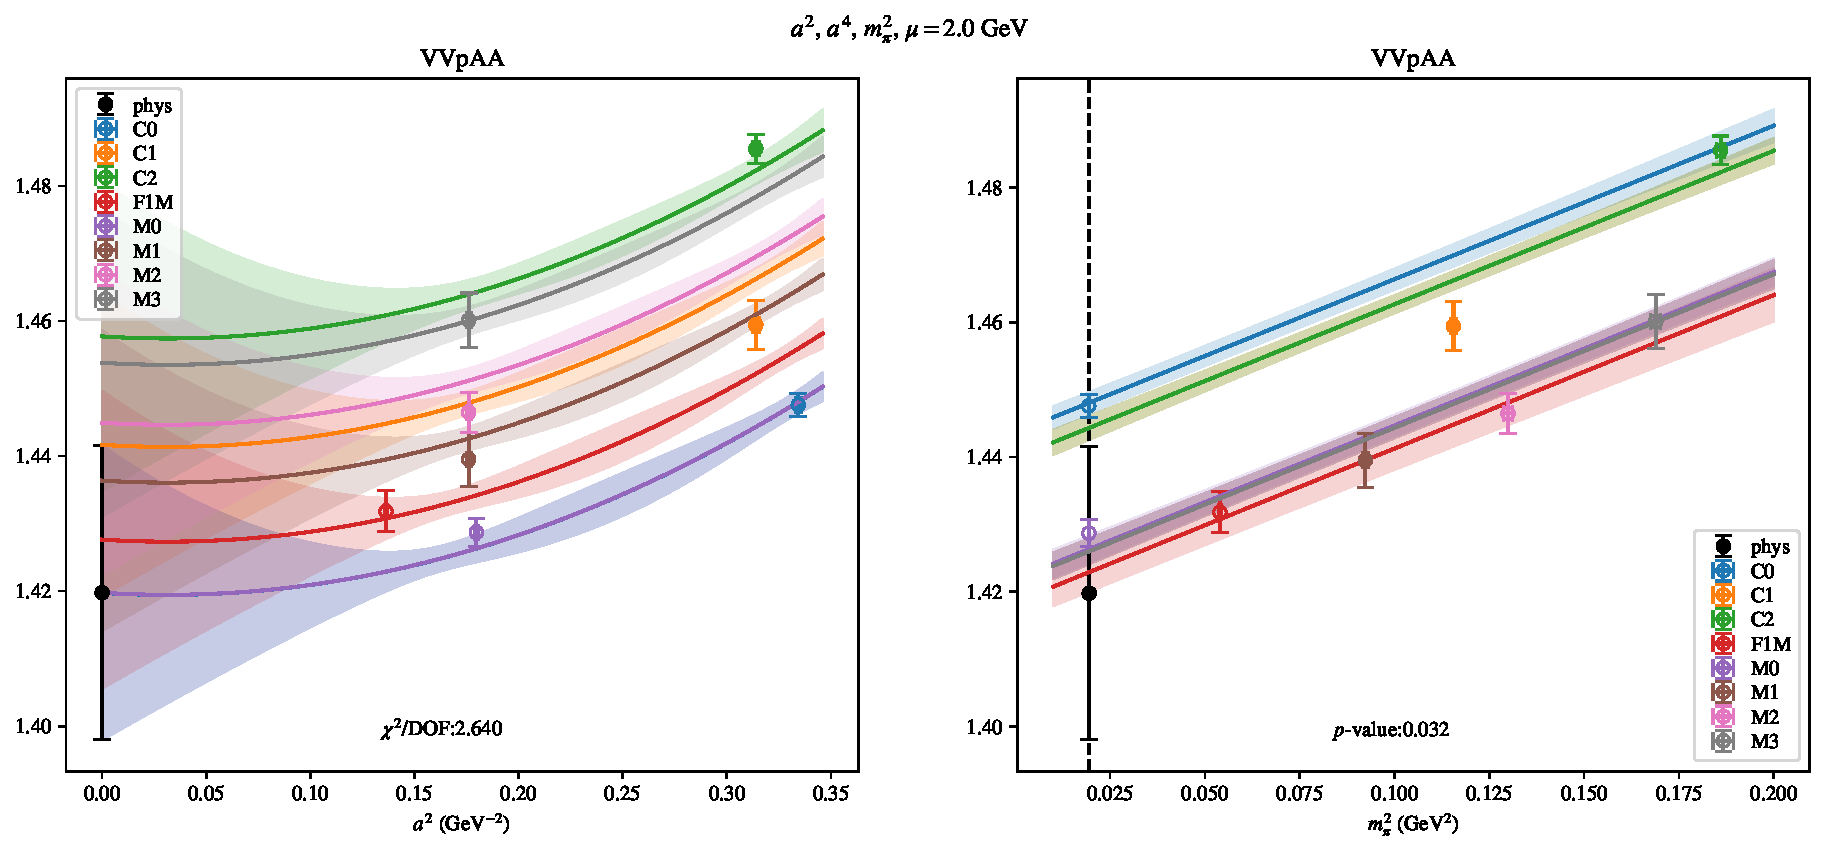
\includepdf[link, pages=-]{VVpAA/NPR/a2a4m2_20.pdf}
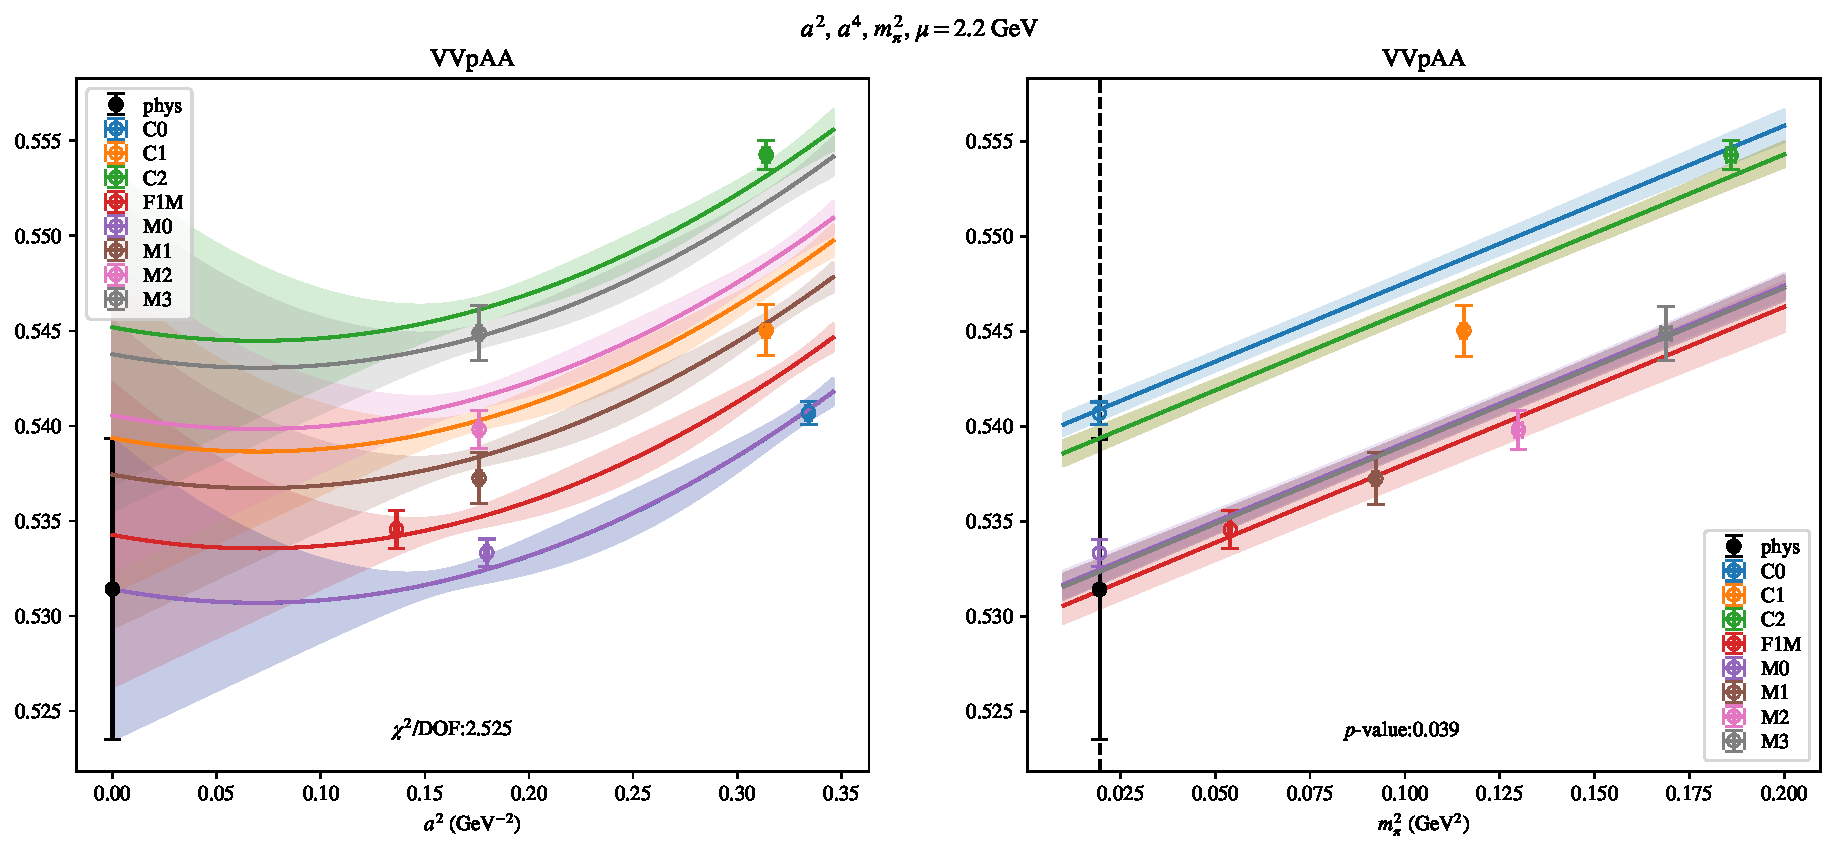
\includepdf[link, pages=-]{VVpAA/NPR/a2a4m2_22.pdf}
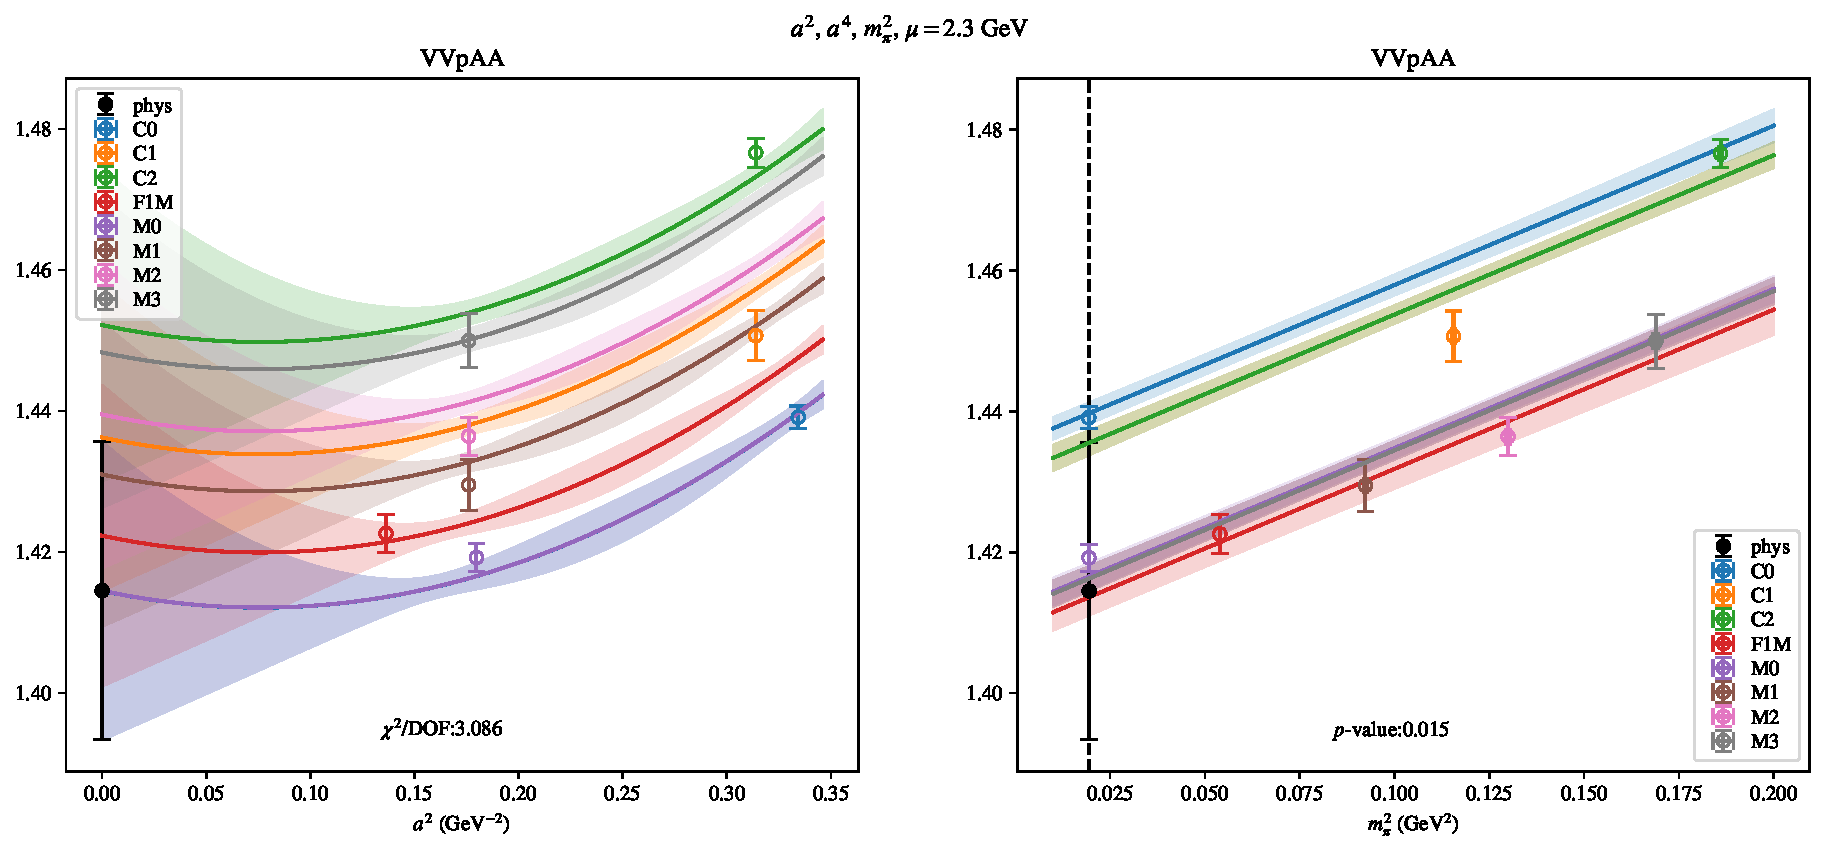
\includepdf[link, pages=-]{VVpAA/NPR/a2a4m2_23.pdf}
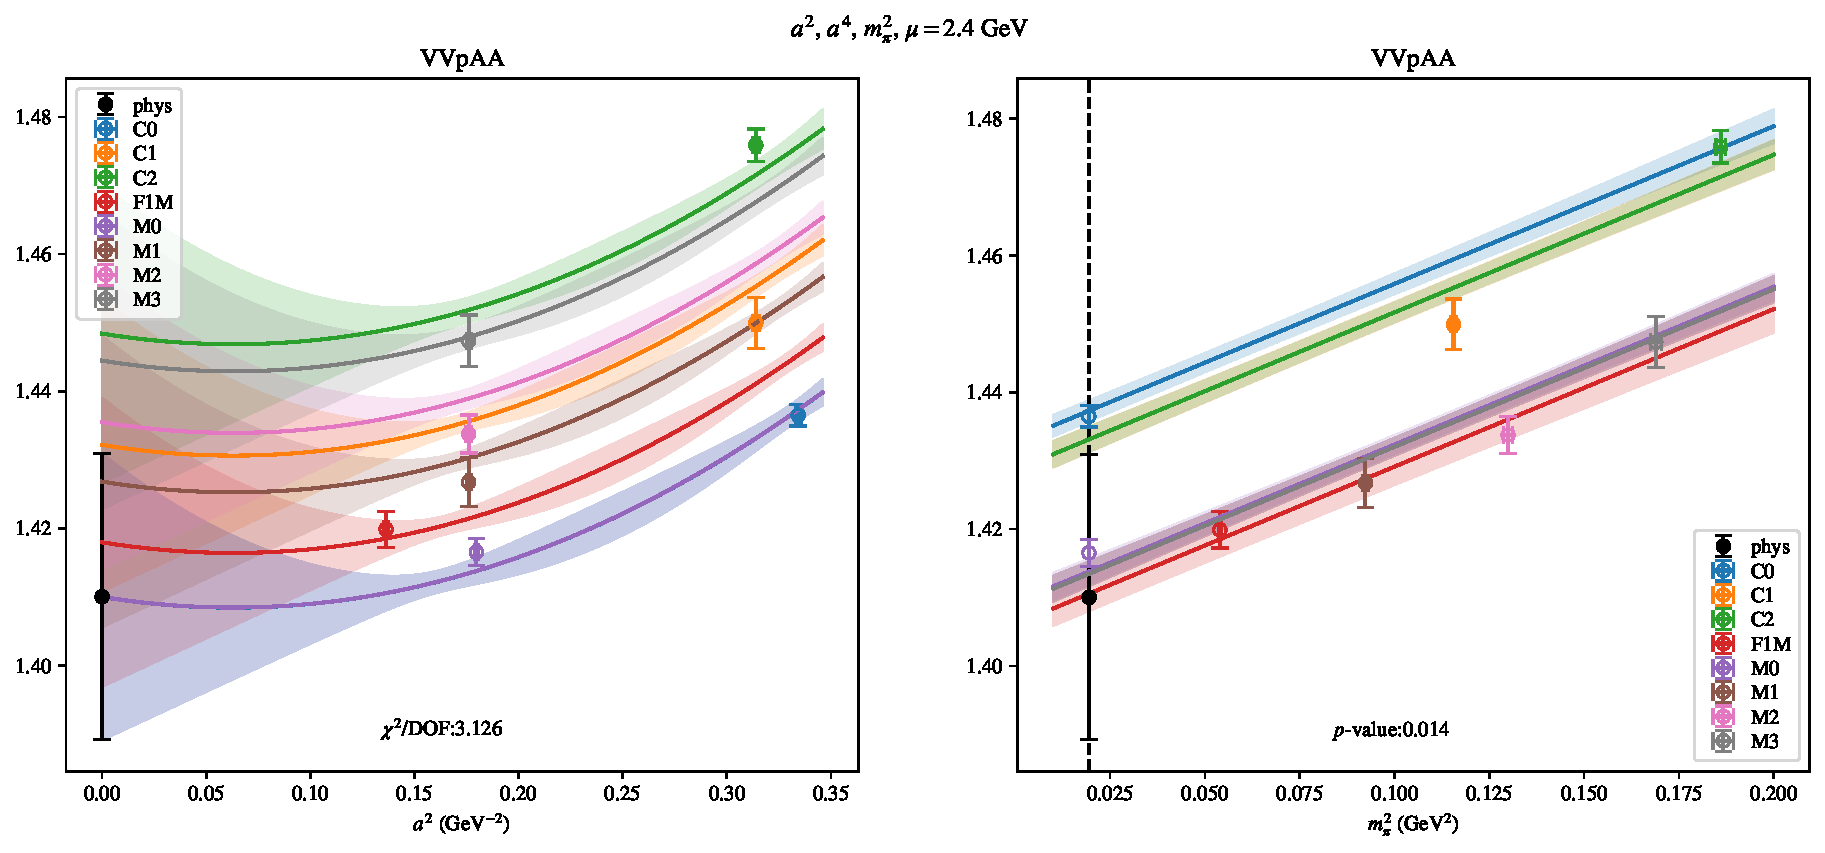
\includepdf[link, pages=-]{VVpAA/NPR/a2a4m2_24.pdf}
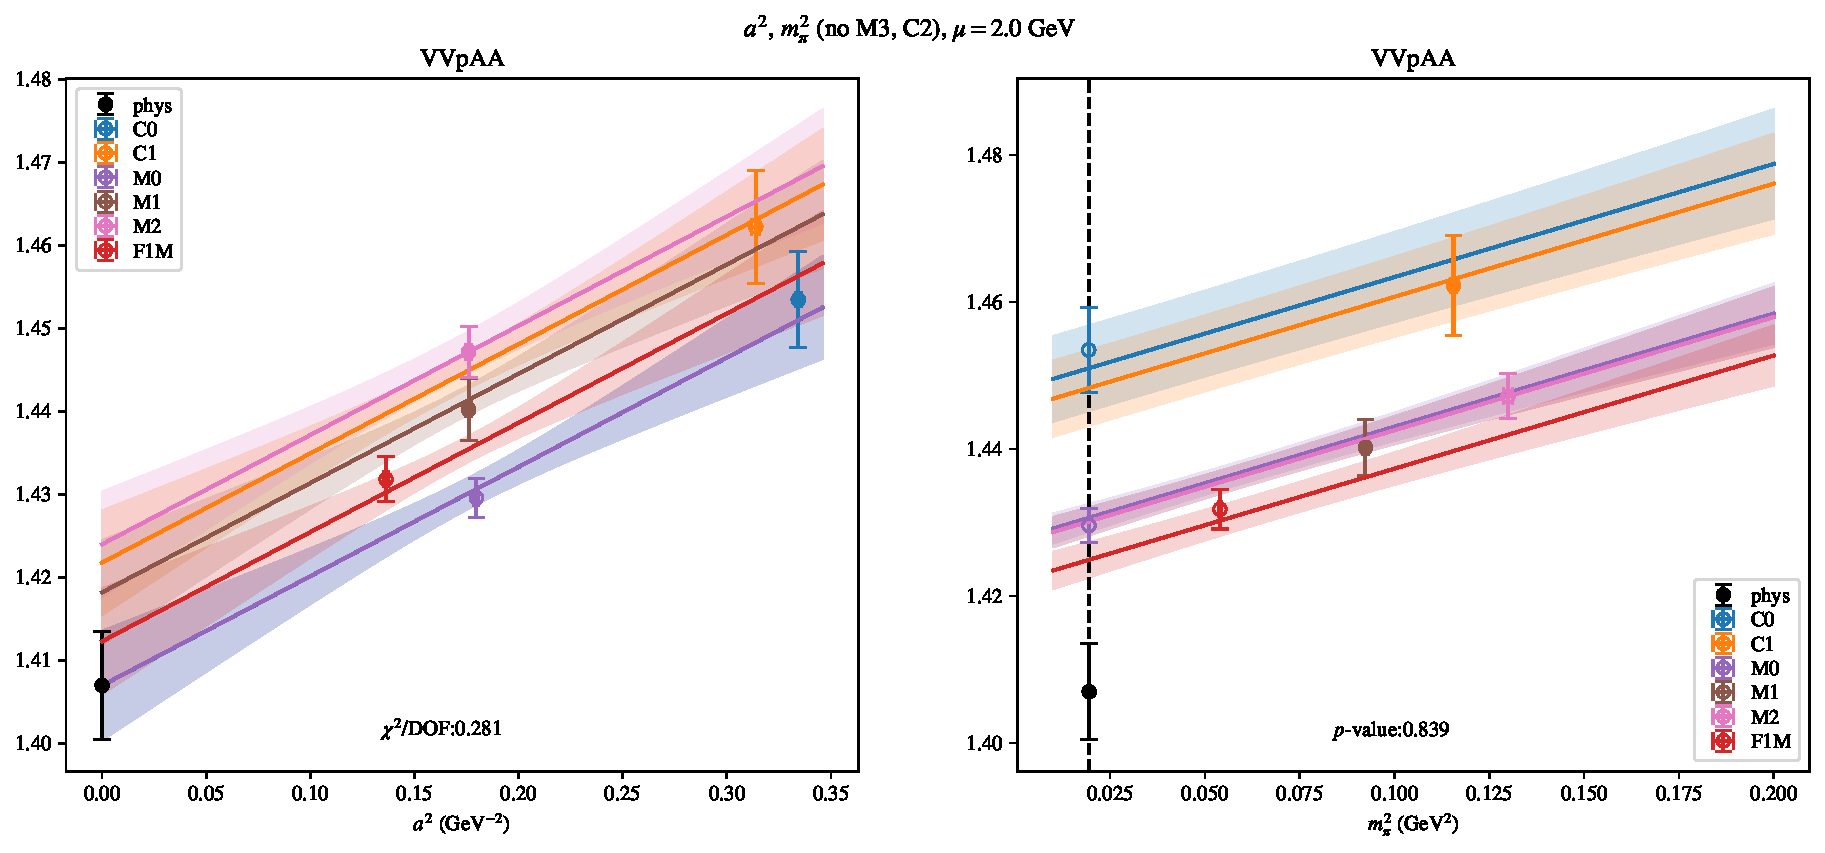
\includepdf[link, pages=-]{VVpAA/NPR/a2m2mcut_20.pdf}
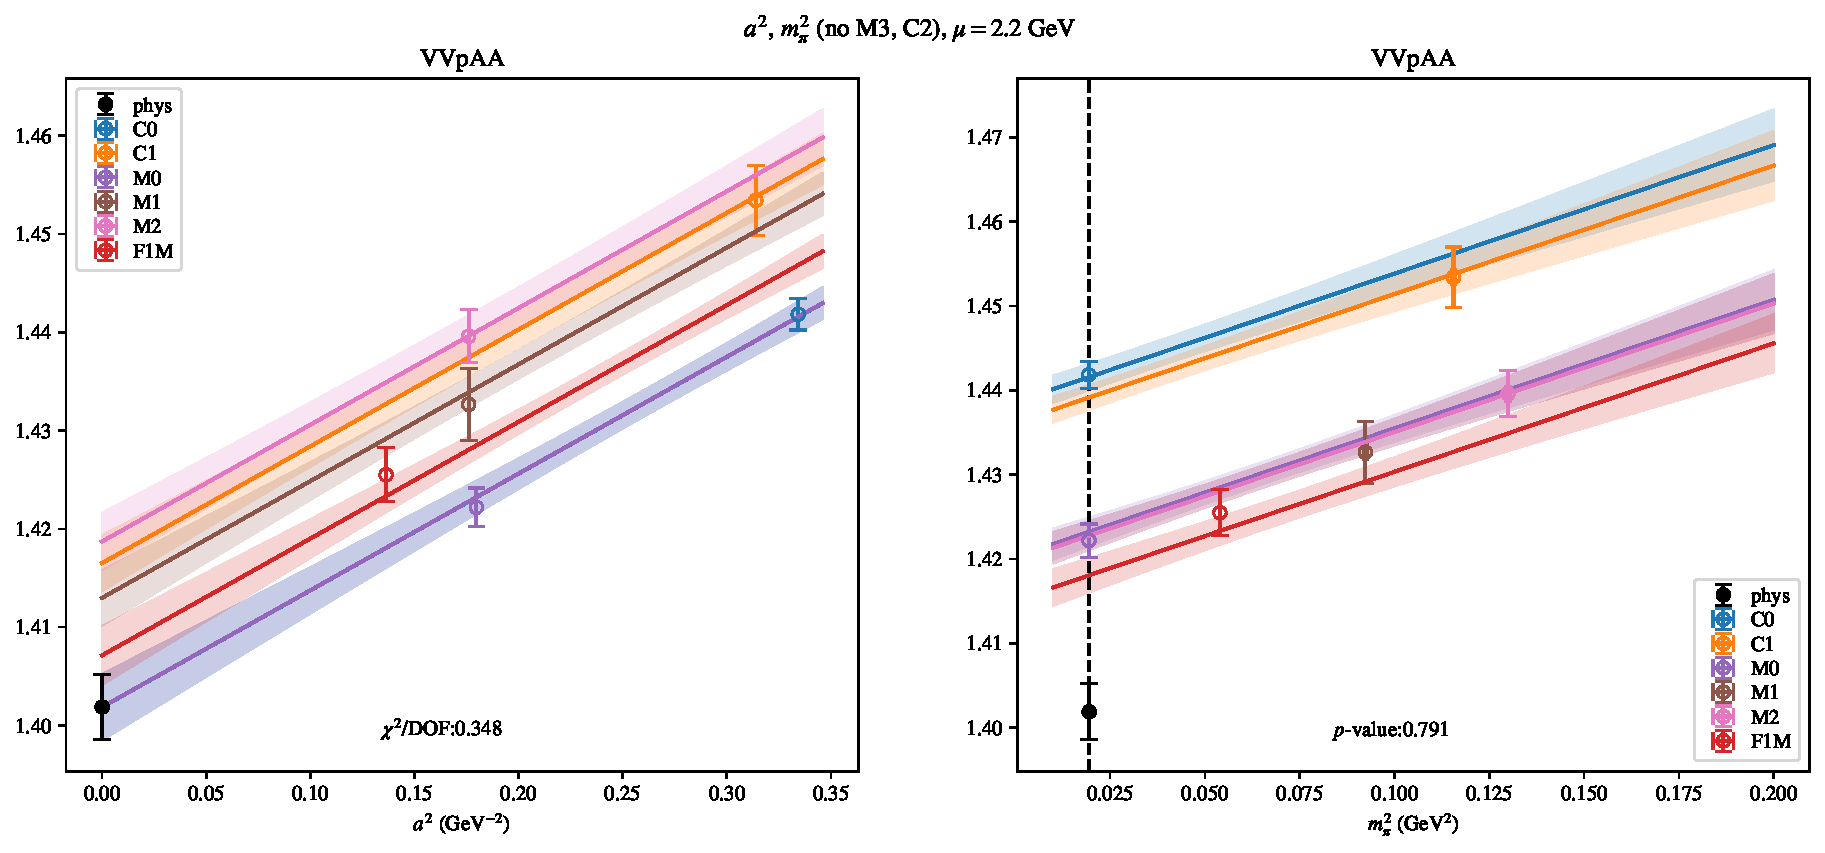
\includepdf[link, pages=-]{VVpAA/NPR/a2m2mcut_22.pdf}
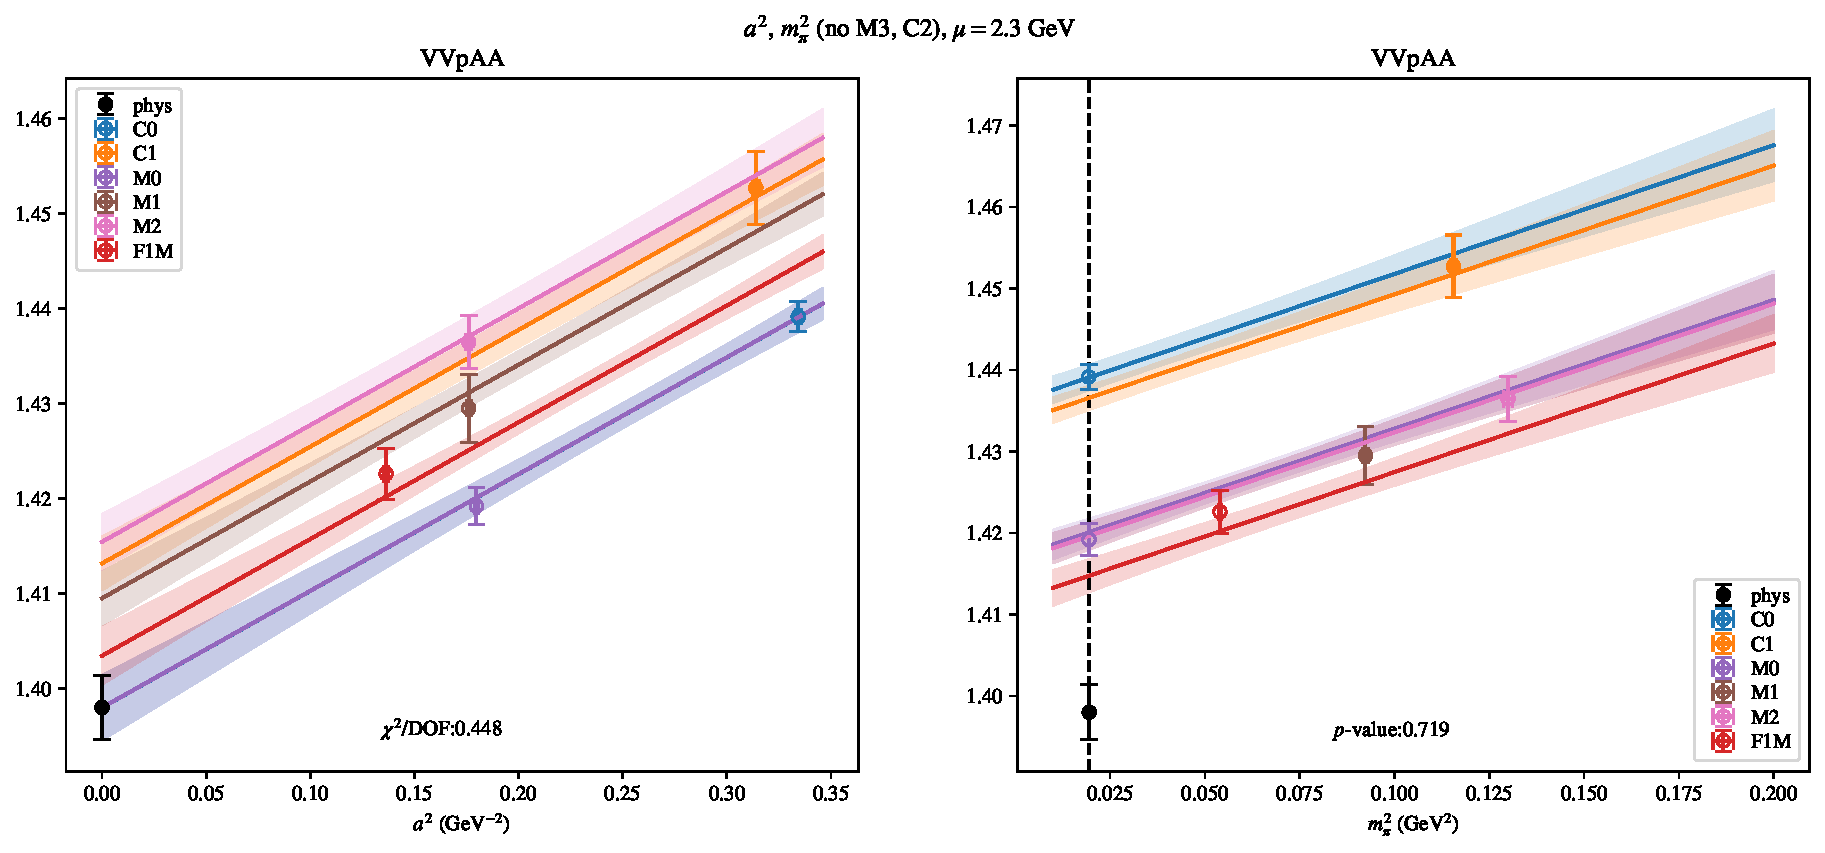
\includepdf[link, pages=-]{VVpAA/NPR/a2m2mcut_23.pdf}
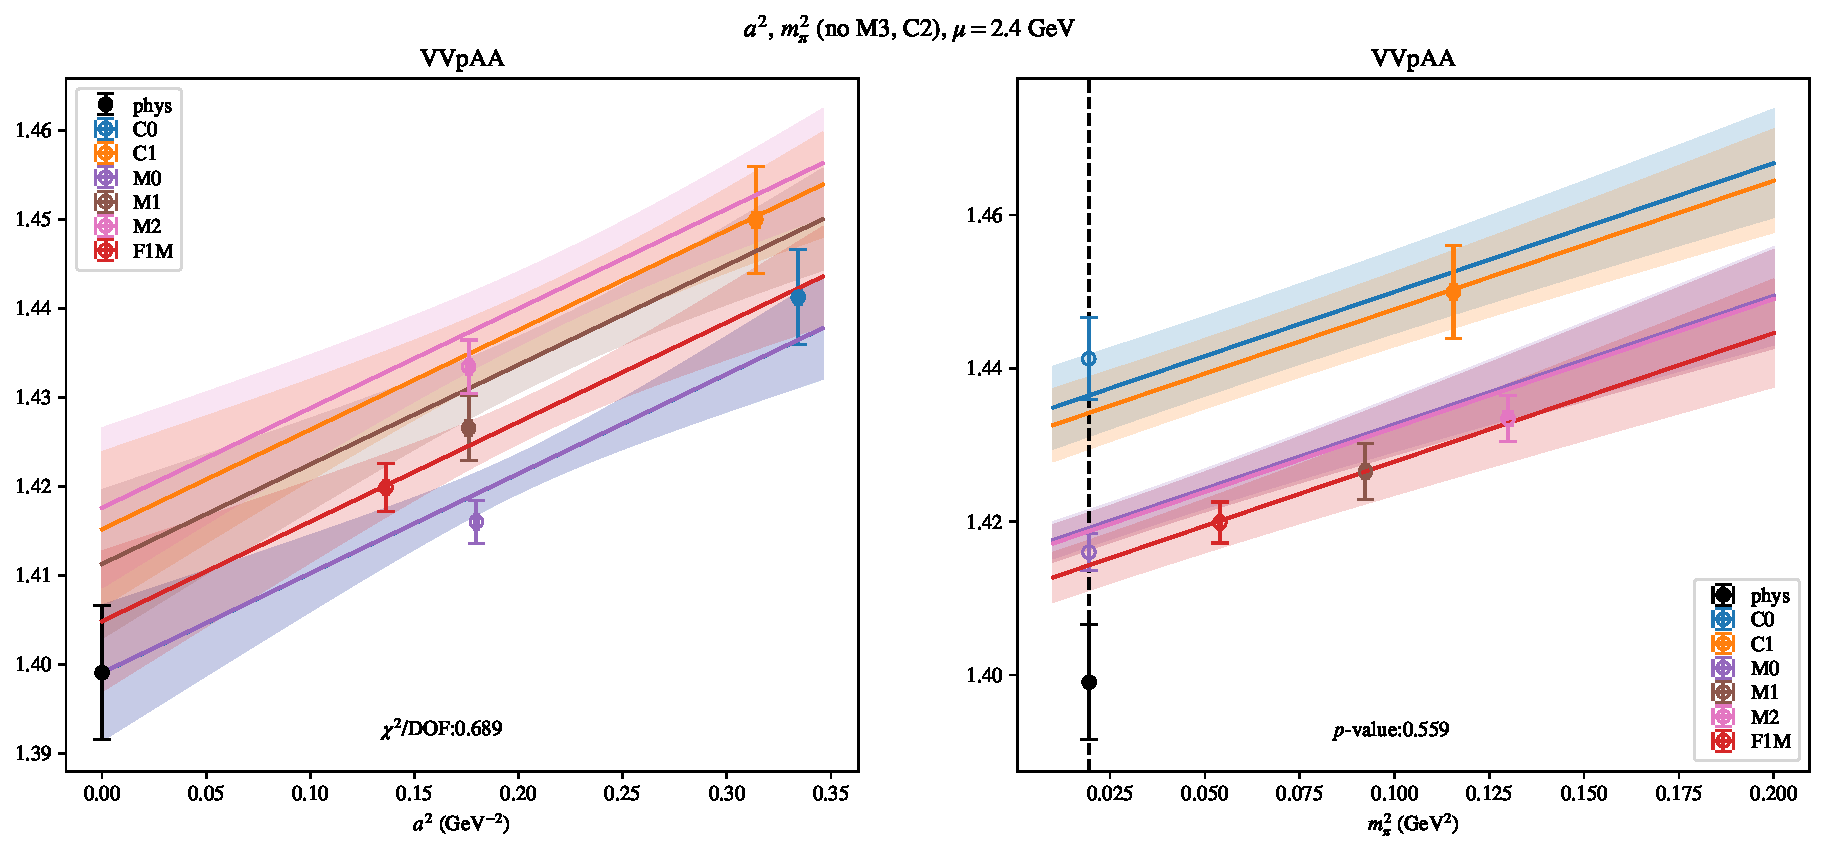
\includepdf[link, pages=-]{VVpAA/NPR/a2m2mcut_24.pdf}
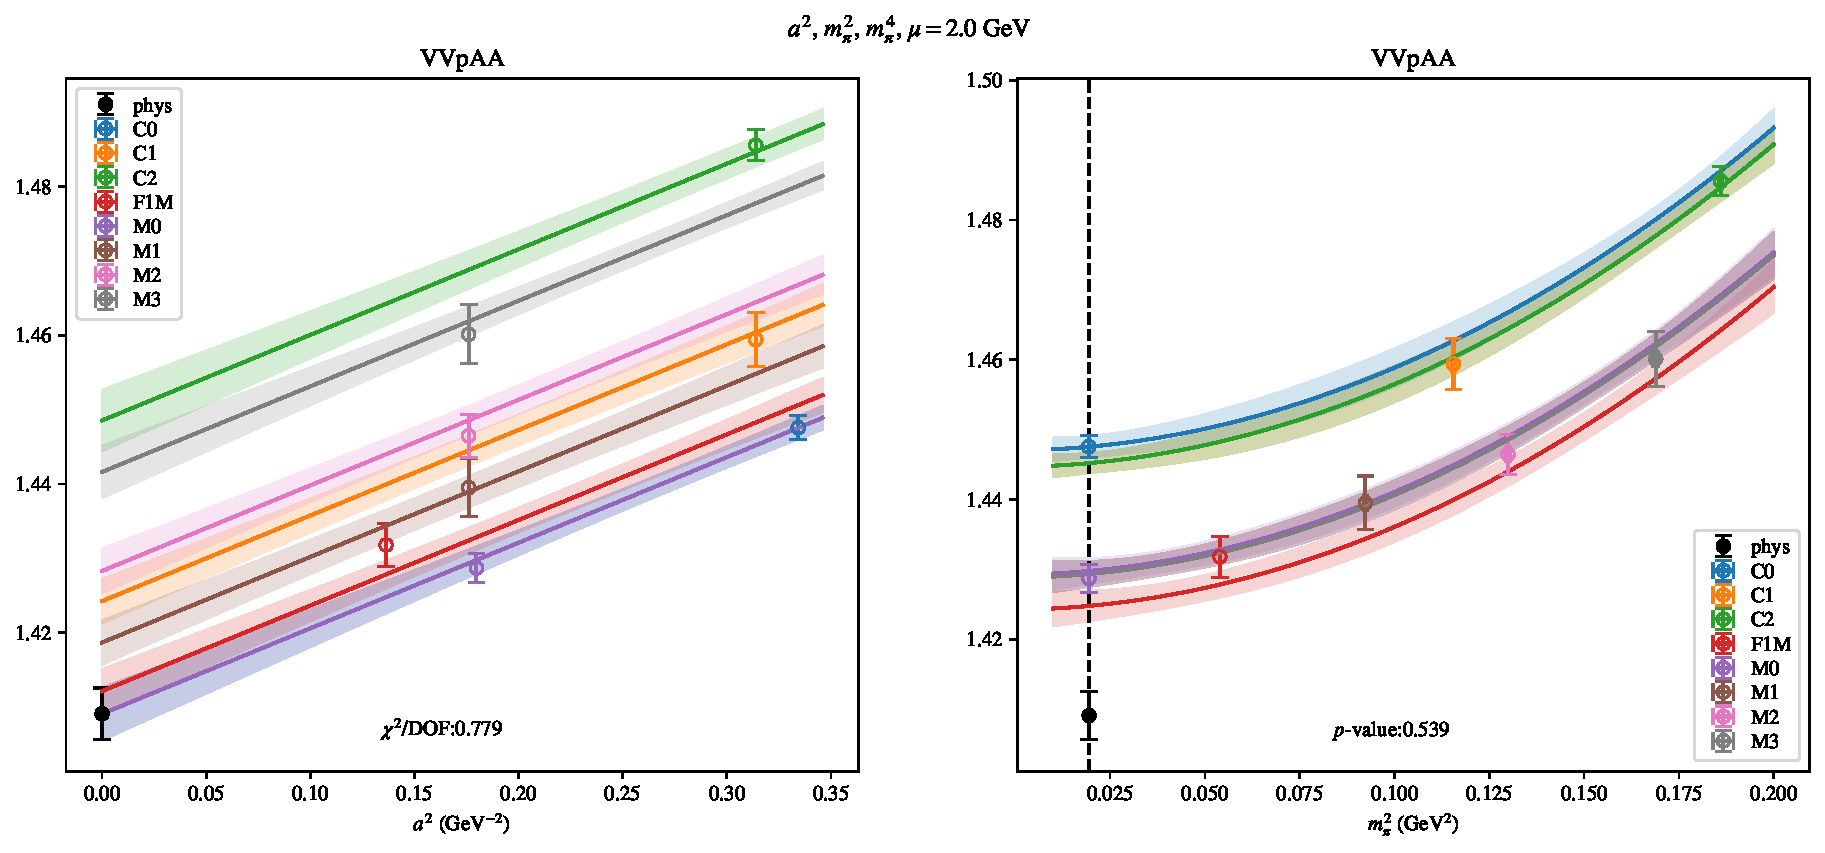
\includepdf[link, pages=-]{VVpAA/NPR/a2m2m4_20.pdf}
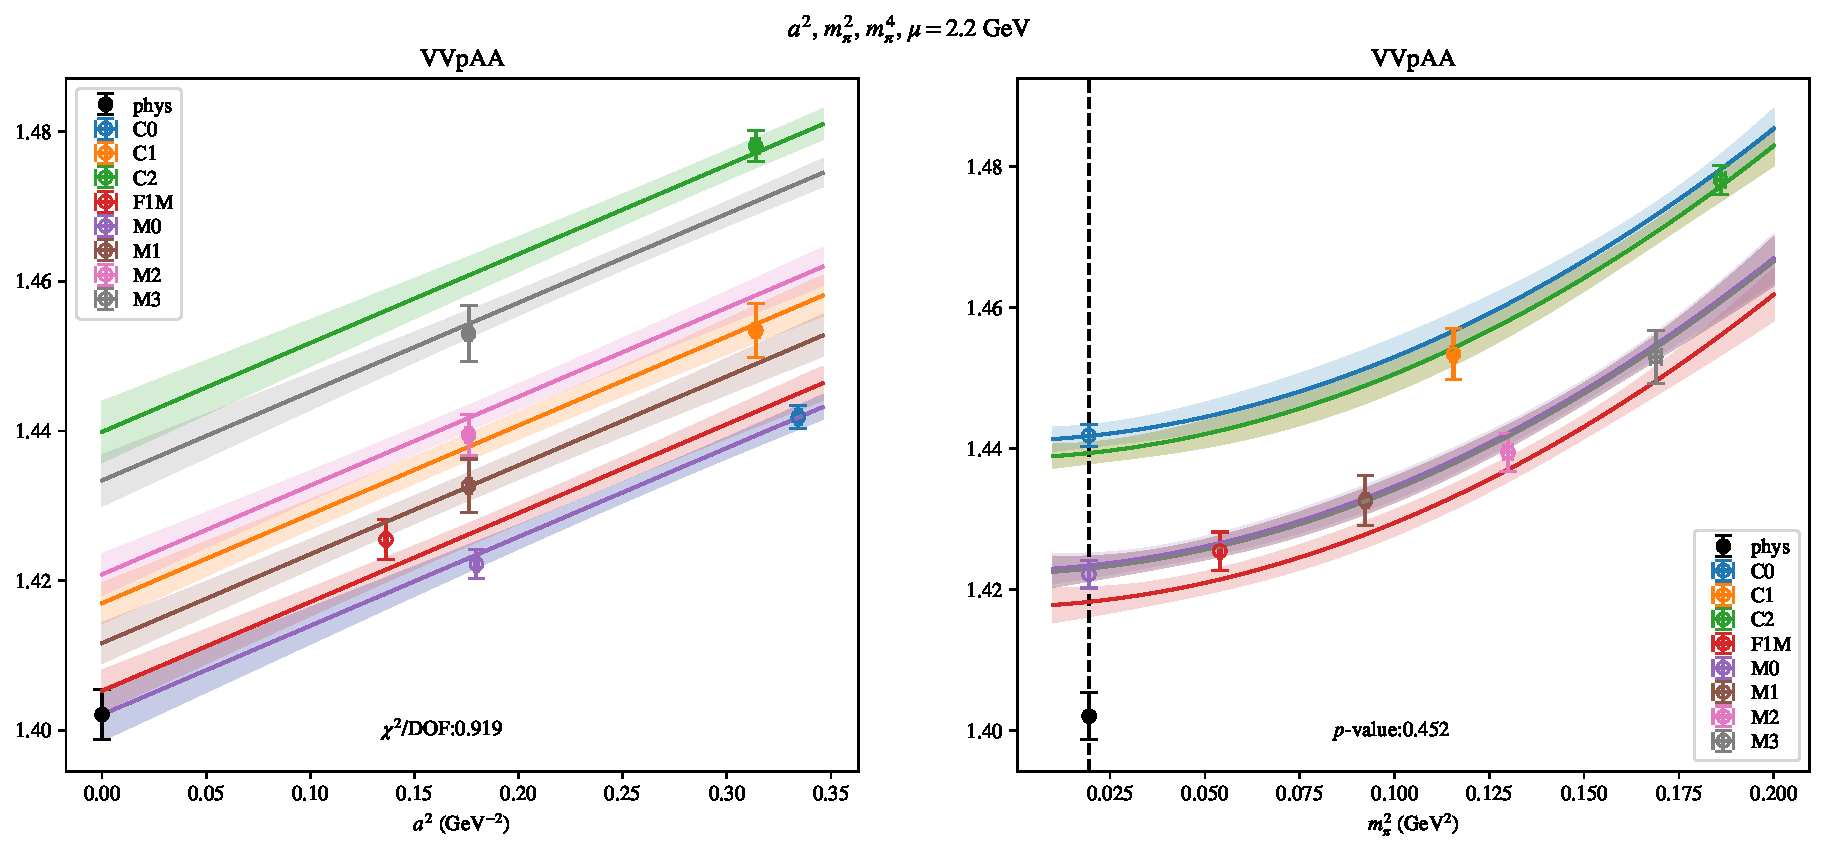
\includepdf[link, pages=-]{VVpAA/NPR/a2m2m4_22.pdf}
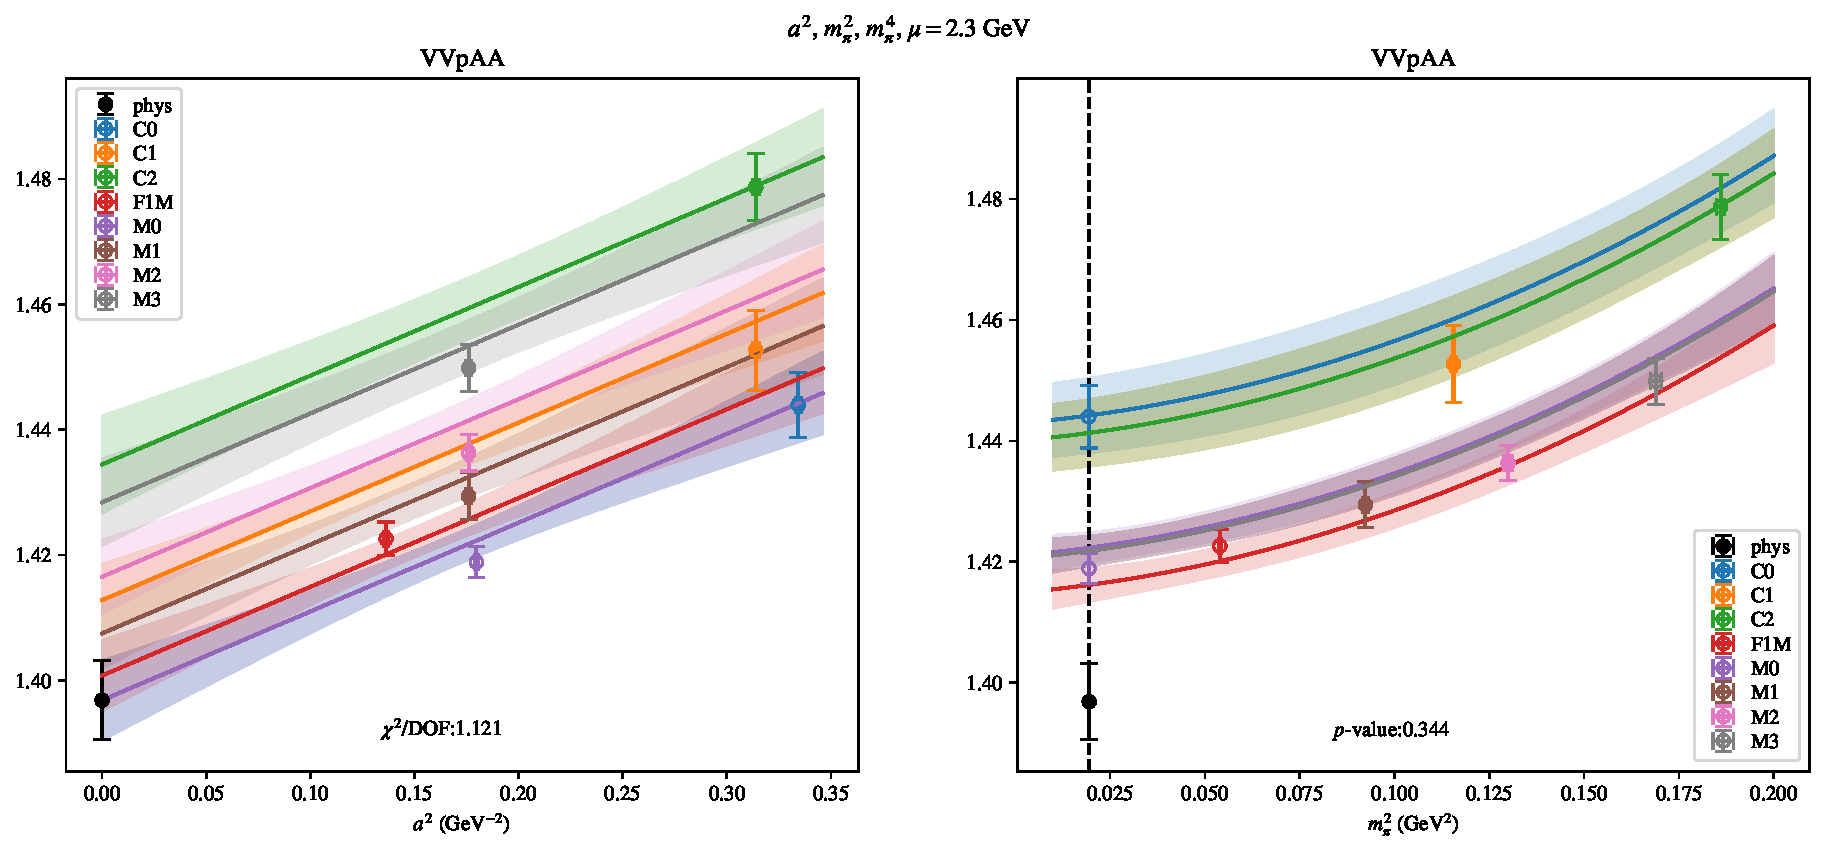
\includepdf[link, pages=-]{VVpAA/NPR/a2m2m4_23.pdf}
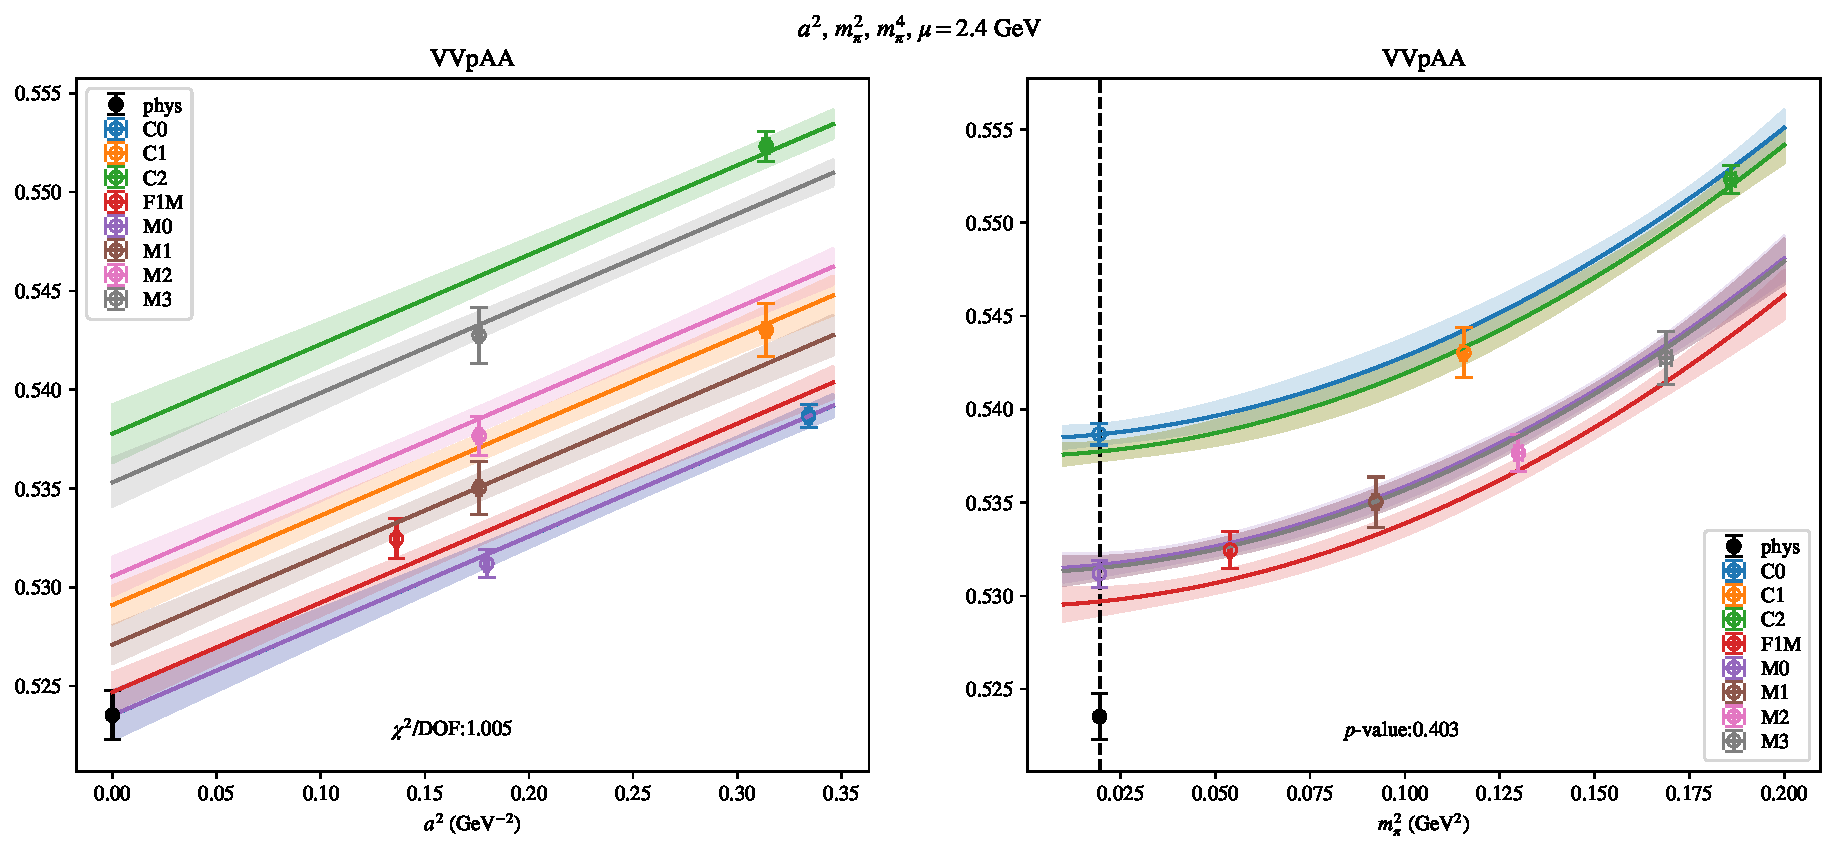
\includepdf[link, pages=-]{VVpAA/NPR/a2m2m4_24.pdf}
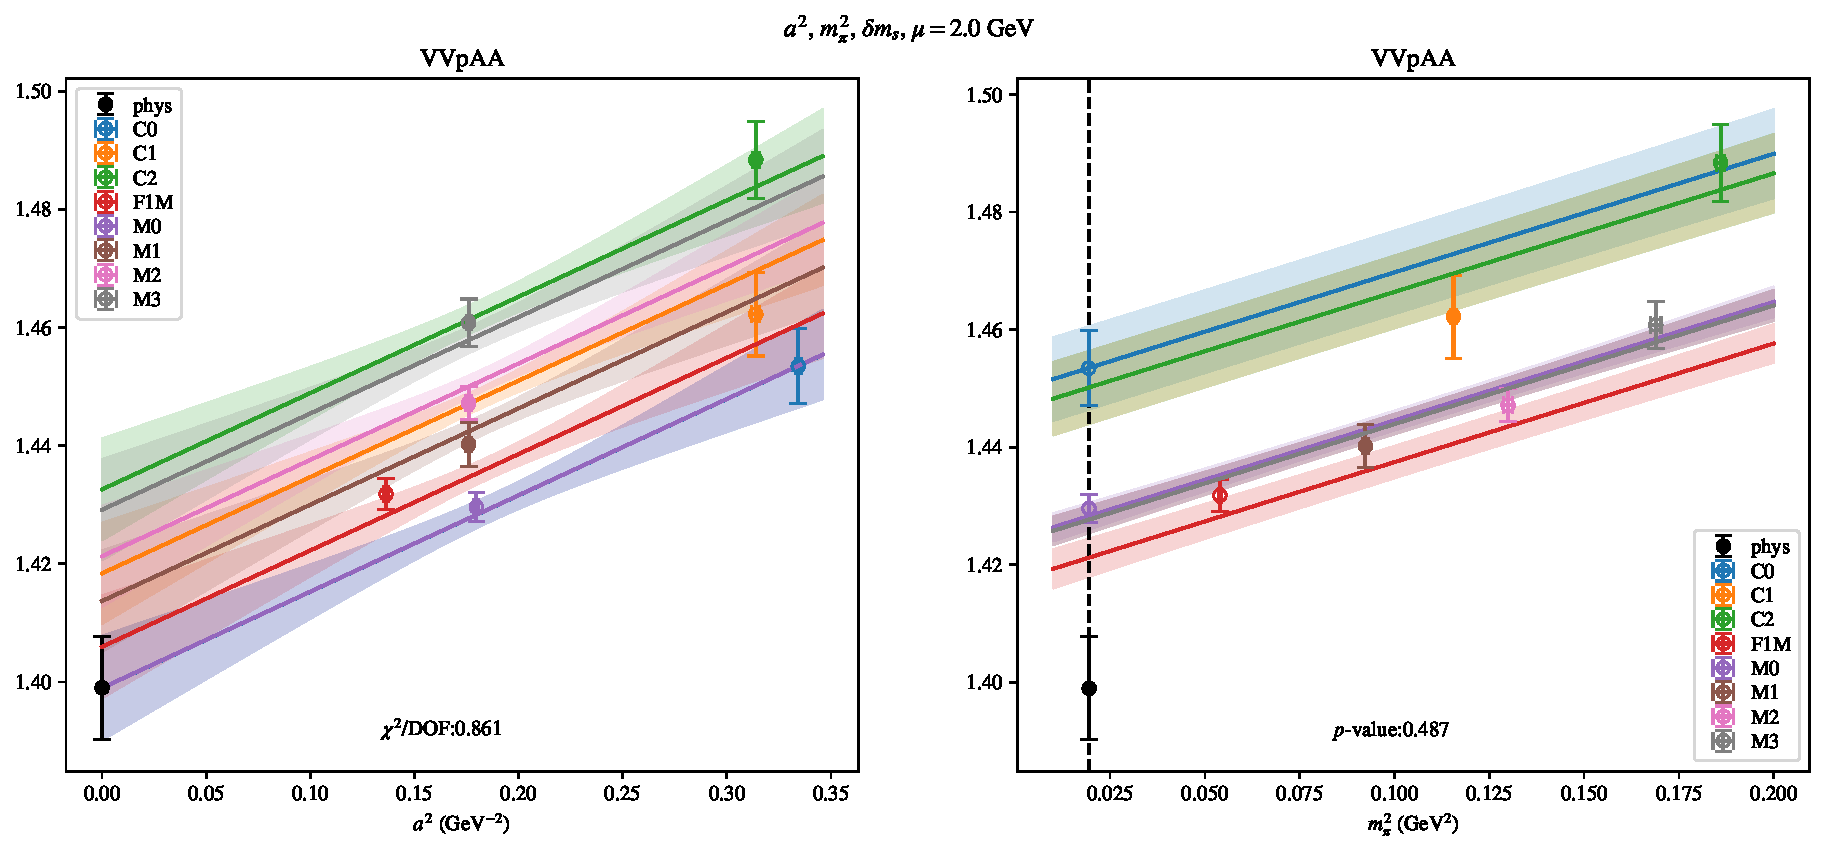
\includepdf[link, pages=-]{VVpAA/NPR/a2m2delm_20.pdf}
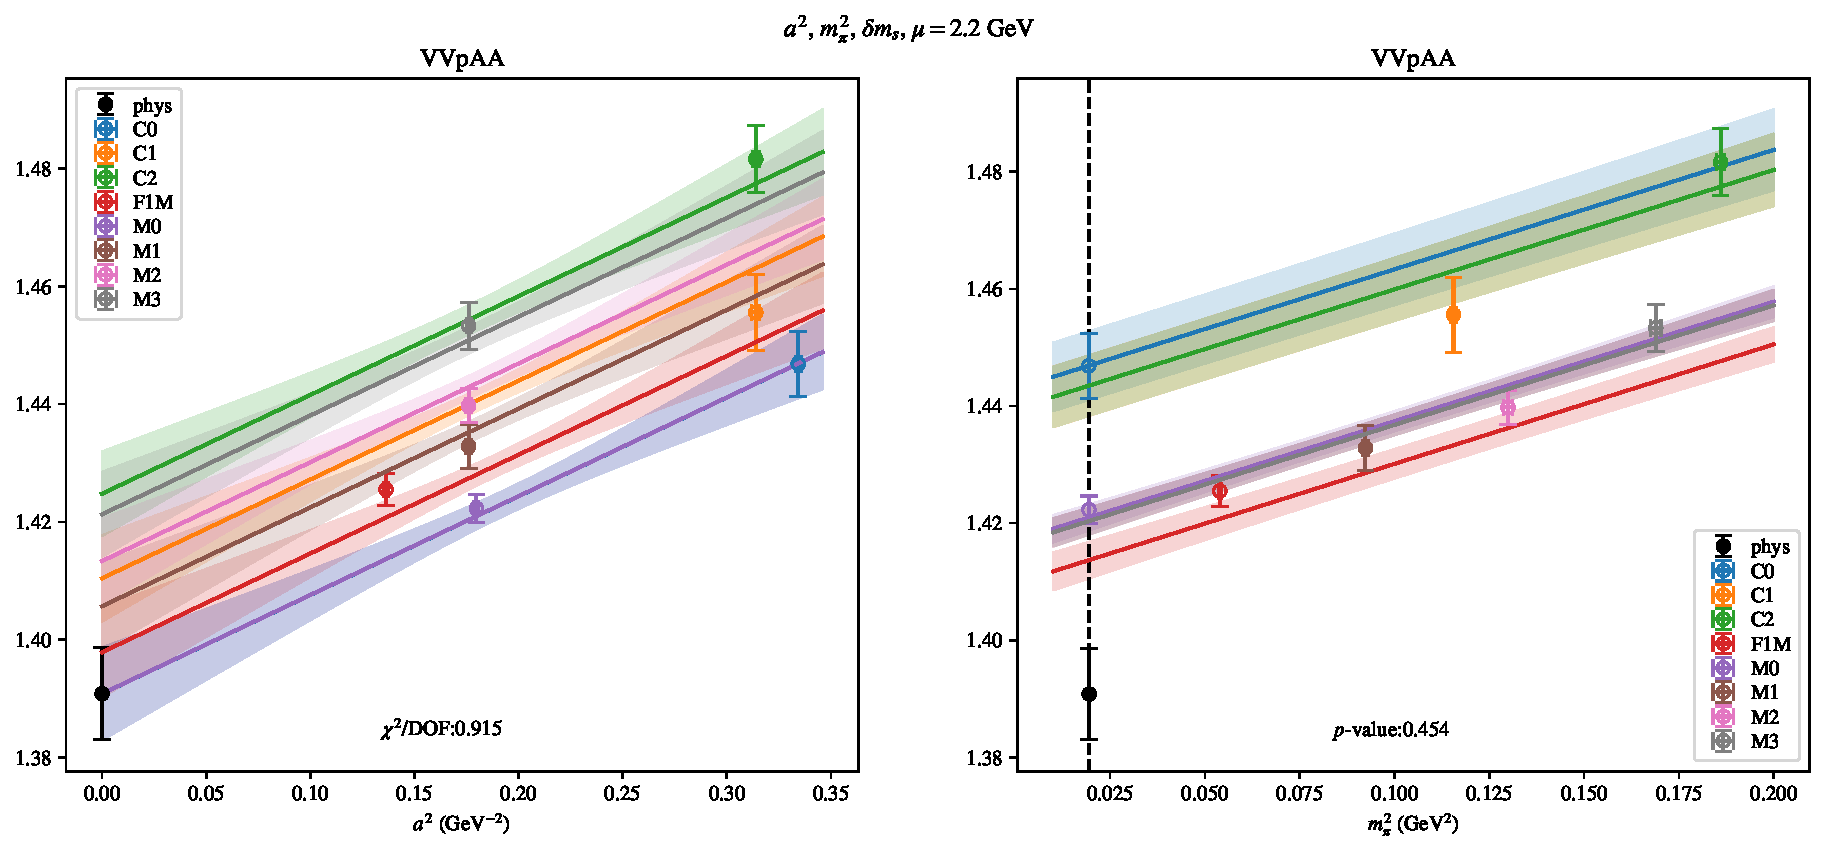
\includepdf[link, pages=-]{VVpAA/NPR/a2m2delm_22.pdf}
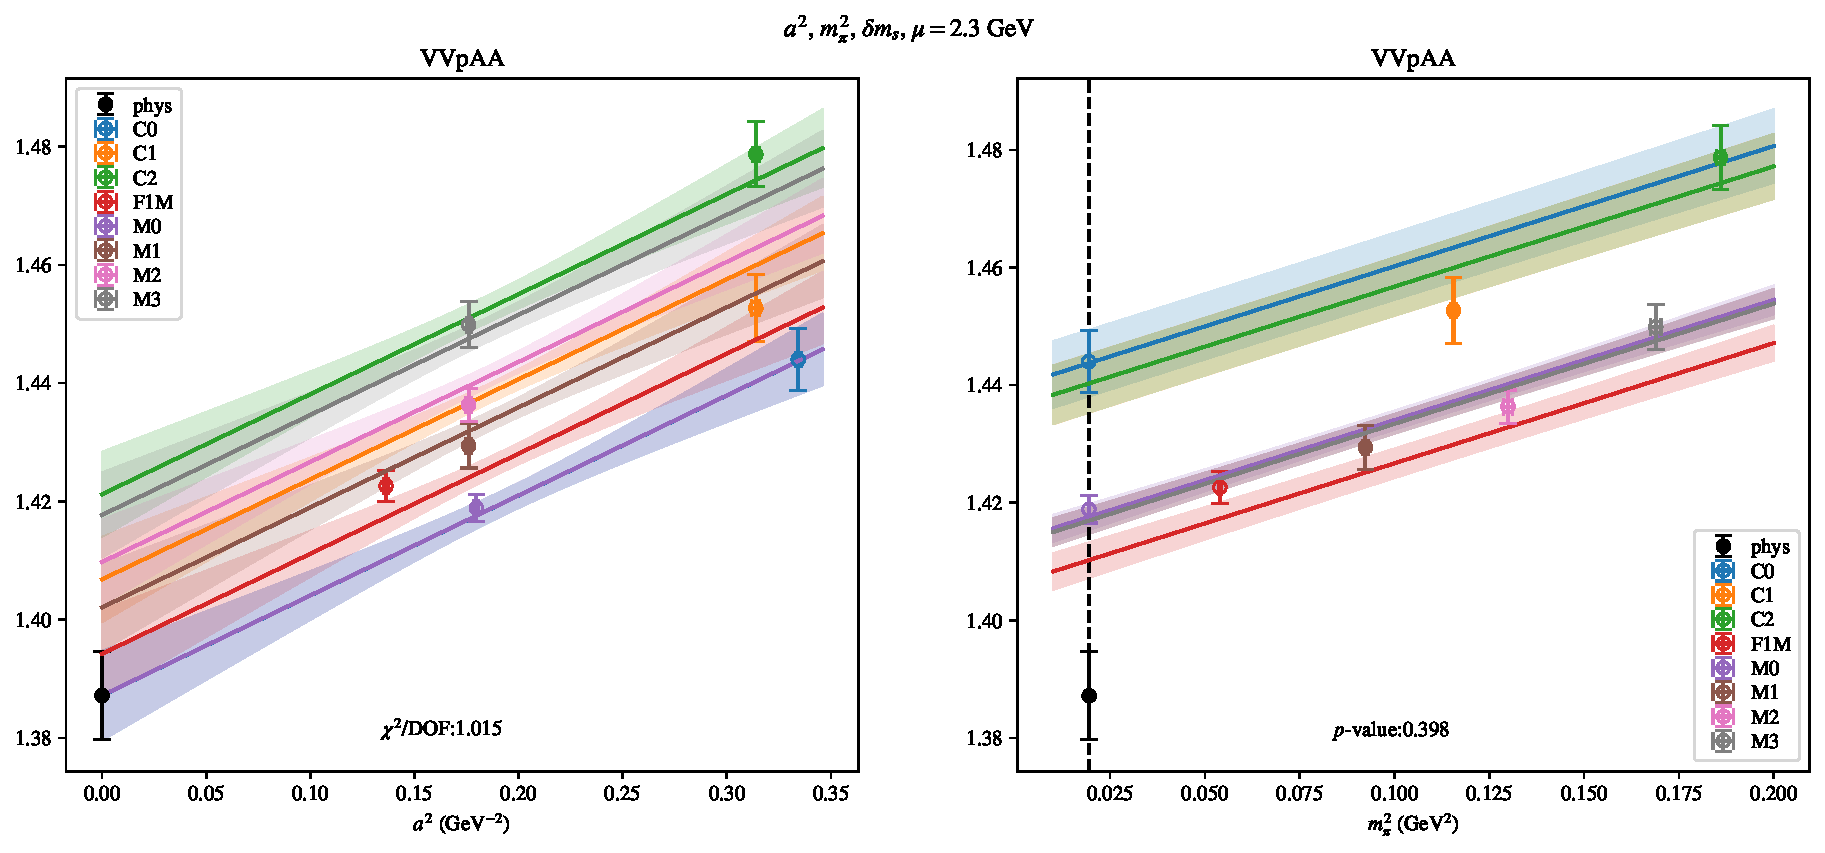
\includepdf[link, pages=-]{VVpAA/NPR/a2m2delm_23.pdf}
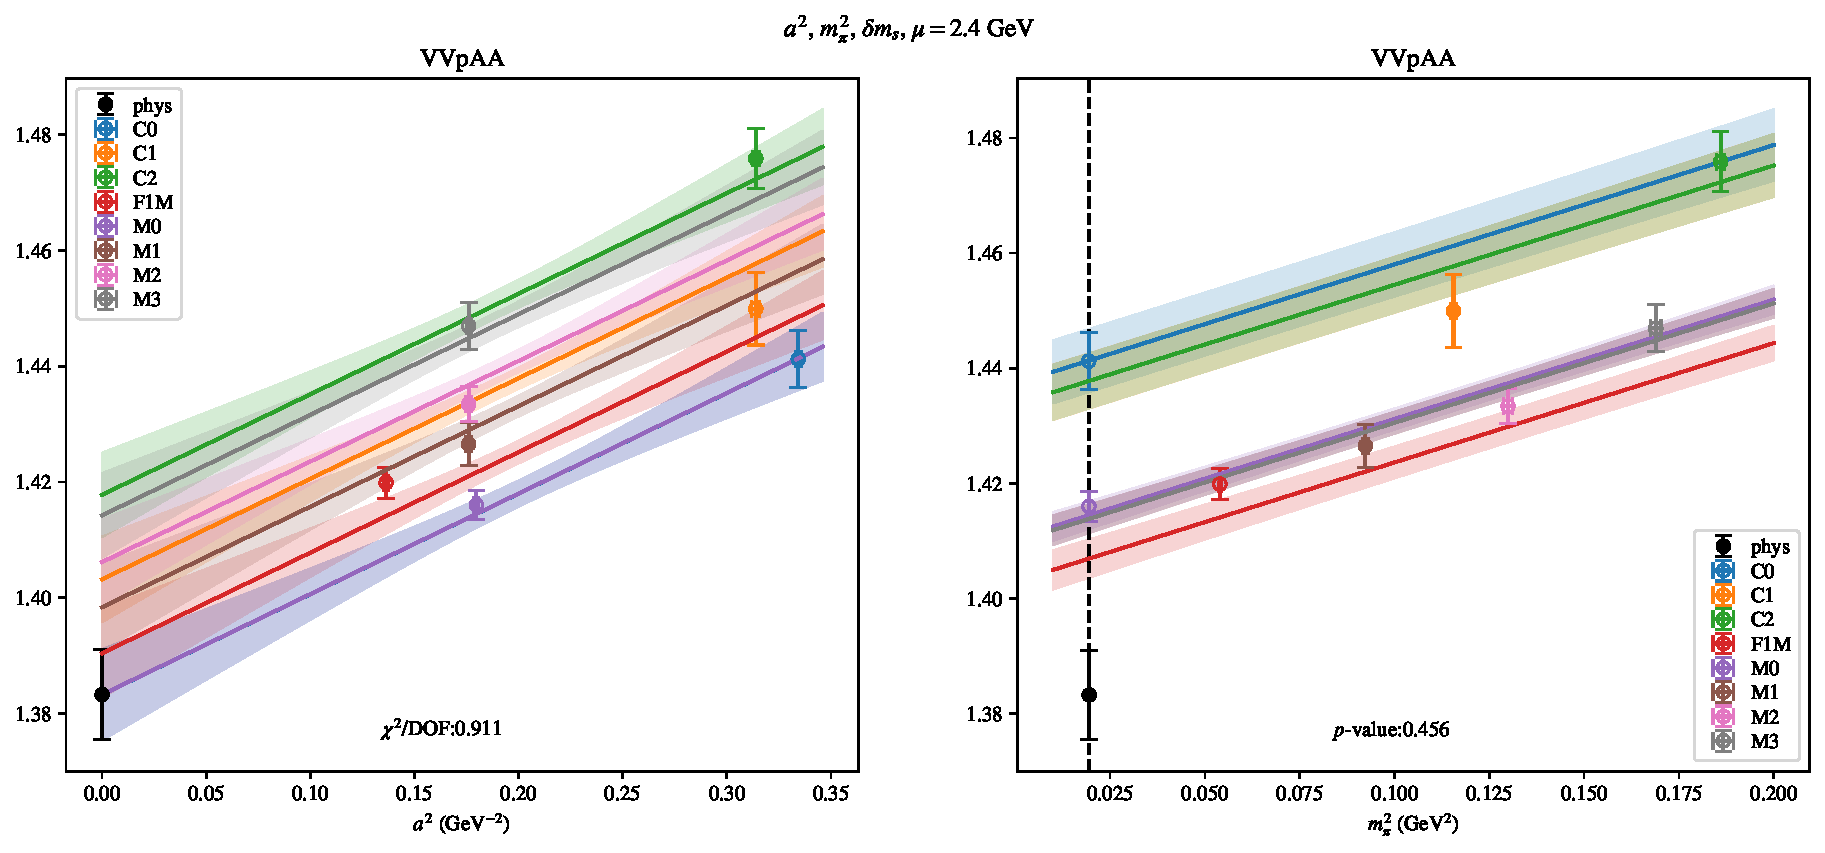
\includepdf[link, pages=-]{VVpAA/NPR/a2m2delm_24.pdf}
\clearpage
\section{$\mathcal{B}_2$}
\begin{table}[h!]
\begin{center}
\begin{tabular}{|c|c|c|c|c|c|c|}
\hline
$\mu$ (GeV) & $a^2$, $m_\pi^2$& $a^2$, $m_\pi^2$ (no C)& $a^2$, $a^4$, $m_\pi^2$& $a^2$, $m_\pi^2$ (no M3, C2)& $a^2$, $m_\pi^2$, $m_\pi^4$& $a^2$, $m_\pi^2$, $\delta m_s$\\
\hline
2.0& \hyperlink{VVmAA/NPR/a2m2_20.pdf.1}{\textbf{-0.991(16)}: 12.581 (0.0)} & \hyperlink{VVmAA/NPR/a2m2noC_20.pdf.1}{\textbf{-0.92(10)}: 0.371 (0.69)} & \hyperlink{VVmAA/NPR/a2a4m2_20.pdf.1}{\textbf{-0.88(14)}: 1.067 (0.371)} & \hyperlink{VVmAA/NPR/a2m2mcut_20.pdf.1}{\textbf{-0.992(16)}: 18.312 (0.0)} & \hyperlink{VVmAA/NPR/a2m2m4_20.pdf.1}{\textbf{-0.994(16)}: 9.718 (0.0)} & \hyperlink{VVmAA/NPR/a2m2delm_20.pdf.1}{\textbf{-0.996(18)}: 0.463 (0.763)}\\
2.2& \hyperlink{VVmAA/NPR/a2m2_22.pdf.1}{\textbf{-1.005(15)}: 10.329 (0.0)} & \hyperlink{VVmAA/NPR/a2m2noC_22.pdf.1}{\textbf{-0.947(91)}: 1.211 (0.298)} & \hyperlink{VVmAA/NPR/a2a4m2_22.pdf.1}{\textbf{-0.91(14)}: 1.276 (0.277)} & \hyperlink{VVmAA/NPR/a2m2mcut_22.pdf.1}{\textbf{-1.006(15)}: 14.819 (0.0)} & \hyperlink{VVmAA/NPR/a2m2m4_22.pdf.1}{\textbf{-1.007(15)}: 8.299 (0.0)} & \hyperlink{VVmAA/NPR/a2m2delm_22.pdf.1}{\textbf{-1.009(17)}: 1.403 (0.23)}\\
2.3& \hyperlink{VVmAA/NPR/a2m2_23.pdf.1}{\textbf{-1.012(15)}: 10.697 (0.0)} & \hyperlink{VVmAA/NPR/a2m2noC_23.pdf.1}{\textbf{-0.954(89)}: 1.585 (0.205)} & \hyperlink{VVmAA/NPR/a2a4m2_23.pdf.1}{\textbf{-0.91(14)}: 1.266 (0.281)} & \hyperlink{VVmAA/NPR/a2m2mcut_23.pdf.1}{\textbf{-1.012(15)}: 15.613 (0.0)} & \hyperlink{VVmAA/NPR/a2m2m4_23.pdf.1}{\textbf{-1.013(15)}: 8.899 (0.0)} & \hyperlink{VVmAA/NPR/a2m2delm_23.pdf.1}{\textbf{-1.015(17)}: 1.92 (0.104)}\\
2.4& \hyperlink{VVmAA/NPR/a2m2_24.pdf.1}{\textbf{-1.016(15)}: 9.874 (0.0)} & \hyperlink{VVmAA/NPR/a2m2noC_24.pdf.1}{\textbf{-0.961(87)}: 1.79 (0.167)} & \hyperlink{VVmAA/NPR/a2a4m2_24.pdf.1}{\textbf{-0.92(13)}: 1.511 (0.196)} & \hyperlink{VVmAA/NPR/a2m2mcut_24.pdf.1}{\textbf{-1.017(15)}: 14.367 (0.0)} & \hyperlink{VVmAA/NPR/a2m2m4_24.pdf.1}{\textbf{-1.018(15)}: 8.351 (0.0)} & \hyperlink{VVmAA/NPR/a2m2delm_24.pdf.1}{\textbf{-1.020(17)}: 1.963 (0.097)}\\
\hline
\end{tabular}
\caption{Physical point value from chiral and continuum extrapolation at renormalisation scale $\mu$. Entries are \textbf{value(error)}: $\chi^2/\text{DOF}$ ($p$-value).}
\end{center}
\end{table}
\begin{table}[h!]
\begin{center}
\begin{tabular}{|c c|c|c|c|c|c|c|}
\hline
$\mu$ (GeV) &  & $a^2$, $m_\pi^2$& $a^2$, $m_\pi^2$ (no C)& $a^2$, $a^4$, $m_\pi^2$& $a^2$, $m_\pi^2$ (no M3, C2)& $a^2$, $m_\pi^2$, $m_\pi^4$& $a^2$, $m_\pi^2$, $\delta m_s$\\
\hline
\multirow{2}{0.5in}{2.0} & $\alpha$ & -0.183(59)& 0.234(64)& 0.87(15)& -0.185(60)& -0.191(60)& -0.199(65)\\
 & $\beta$ & 0.00164(31)& 0.00235(67)& 0.00179(36)& 0.00077(45)& -0.0037(98)& 0.00160(31)\\
\hline
\multirow{2}{0.5in}{2.2} & $\alpha$ & -0.224(57)& 0.116(55)& 0.65(14)& -0.225(56)& -0.229(56)& -0.236(62)\\
 & $\beta$ & 0.00135(21)& 0.00154(52)& 0.00124(25)& 0.00070(33)& -0.0022(85)& 0.00120(21)\\
\hline
\multirow{2}{0.5in}{2.3} & $\alpha$ & -0.245(56)& 0.087(53)& 0.62(14)& -0.247(55)& -0.251(56)& -0.257(62)\\
 & $\beta$ & 0.00145(20)& 0.00153(41)& 0.00135(23)& 0.00088(31)& -0.0018(80)& 0.00126(20)\\
\hline
\multirow{2}{0.5in}{2.4} & $\alpha$ & -0.264(56)& 0.048(51)& 0.54(14)& -0.265(56)& -0.270(56)& -0.275(61)\\
 & $\beta$ & 0.00143(19)& 0.00154(35)& 0.00133(21)& 0.00093(28)& -0.0015(75)& 0.00124(19)\\
\hline
\end{tabular}
\caption{Fit values of coefficients in $Q = Q_{phys} + \mathbf{\alpha} a^2 + \mathbf{\beta}\left(\frac{m_\pi^2}{f_\pi^2}-\frac{m_{\pi,PDG}^2}{f_\pi^2}\right) + \ldots$.}
\end{center}
\end{table}
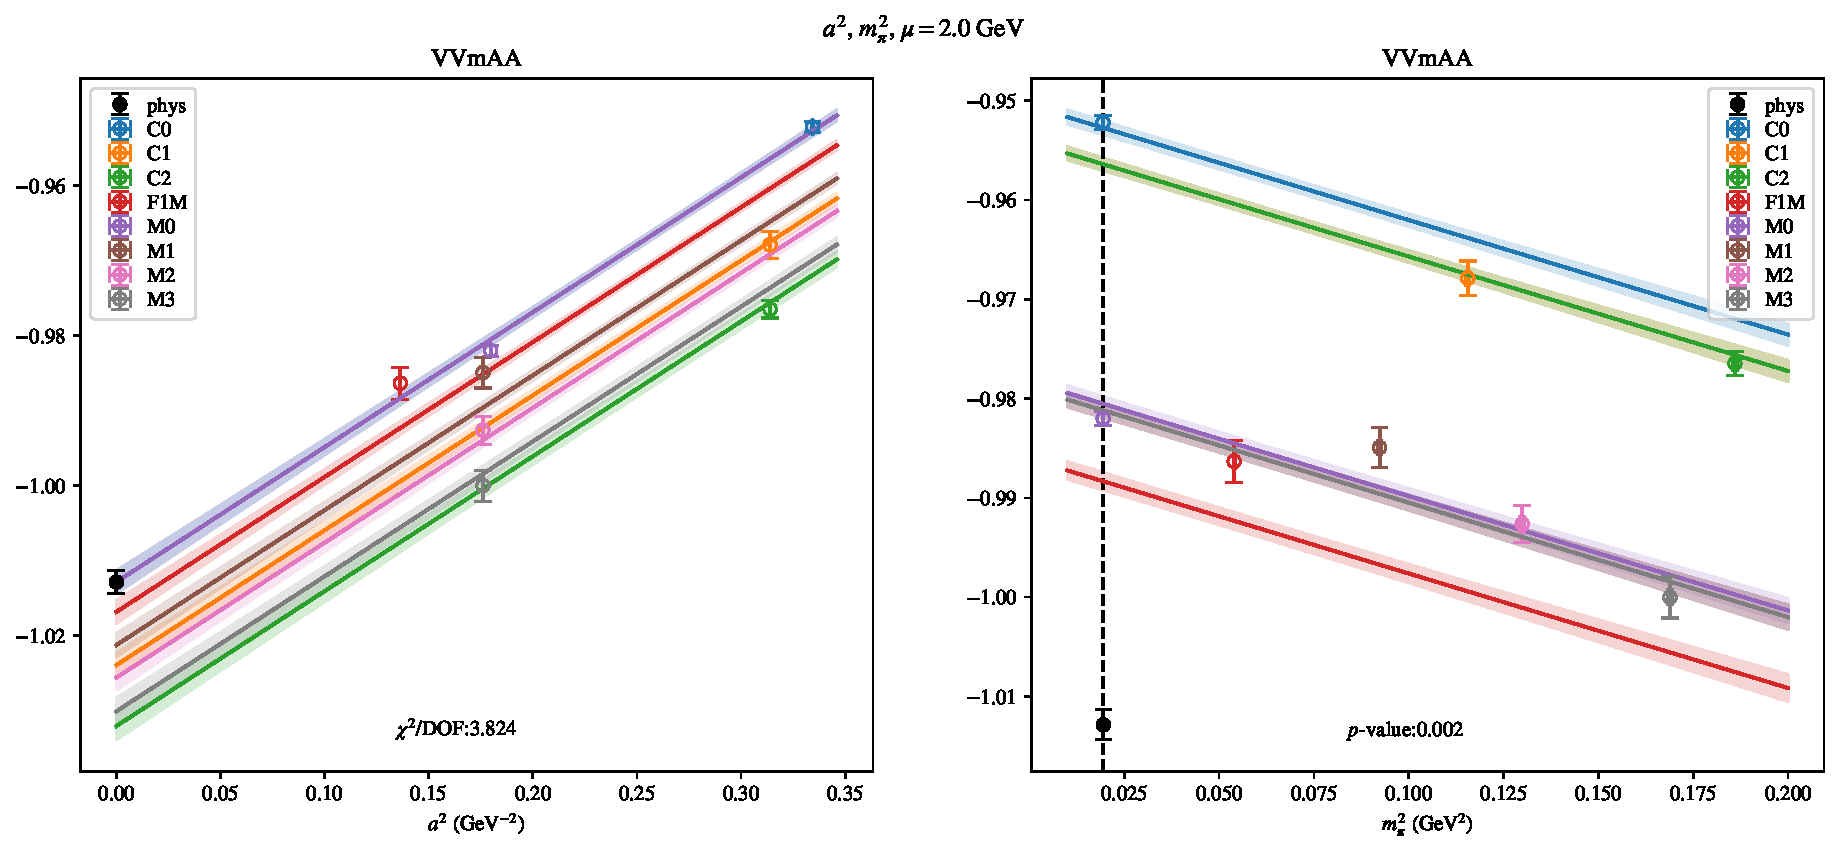
\includepdf[link, pages=-]{VVmAA/NPR/a2m2_20.pdf}
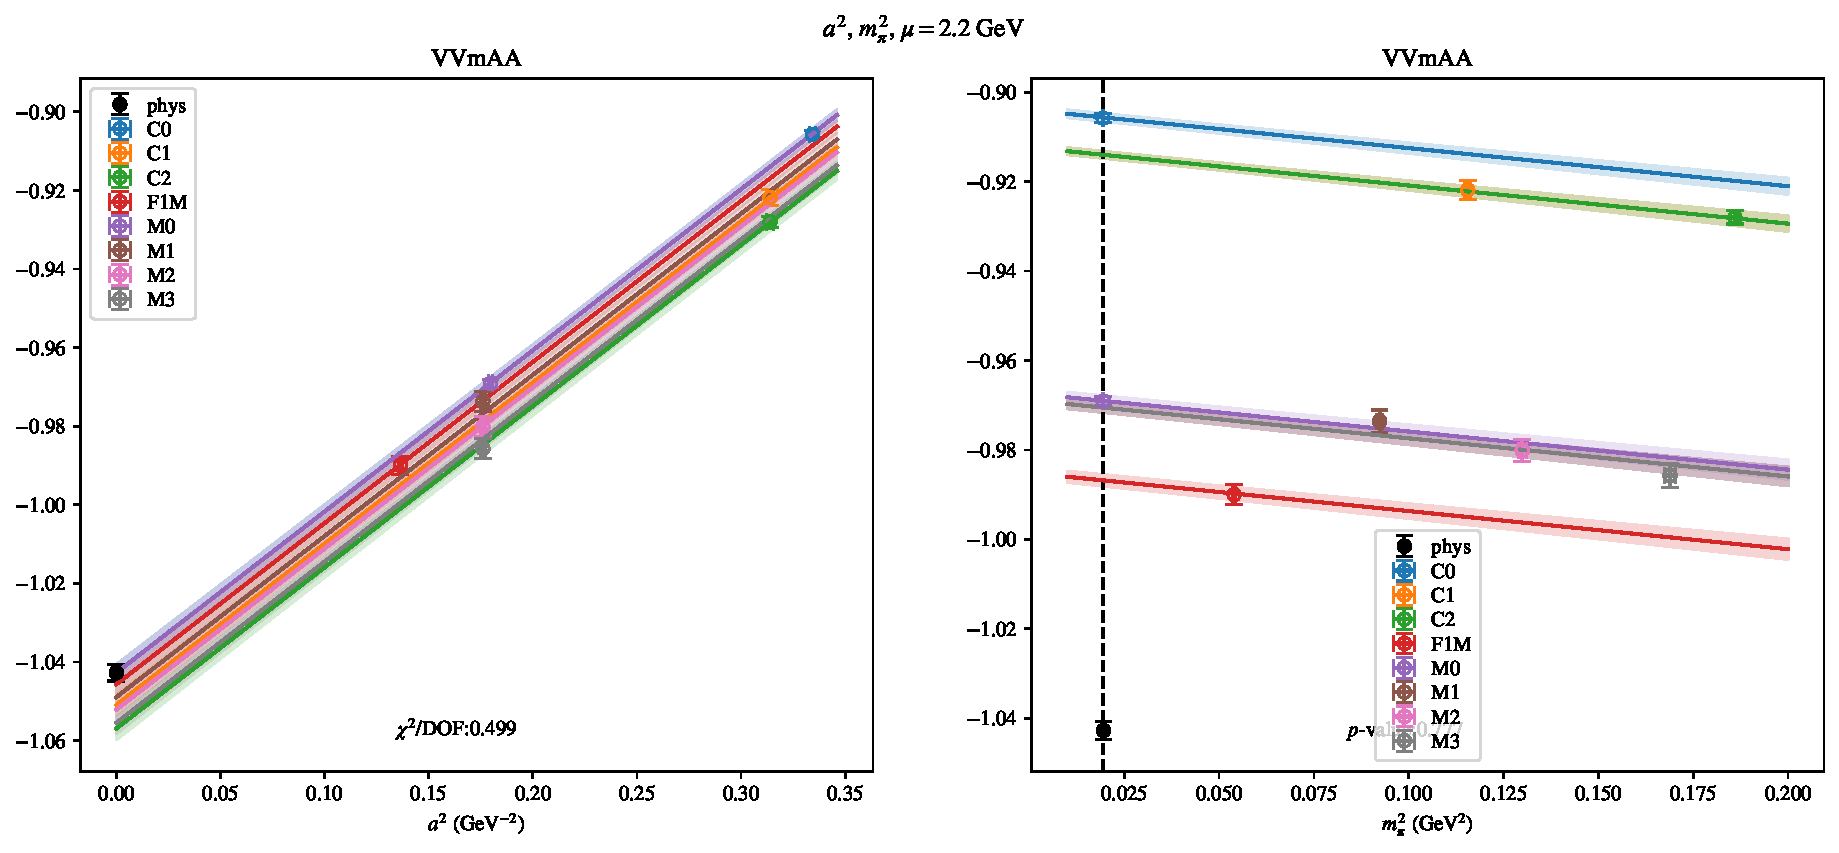
\includepdf[link, pages=-]{VVmAA/NPR/a2m2_22.pdf}
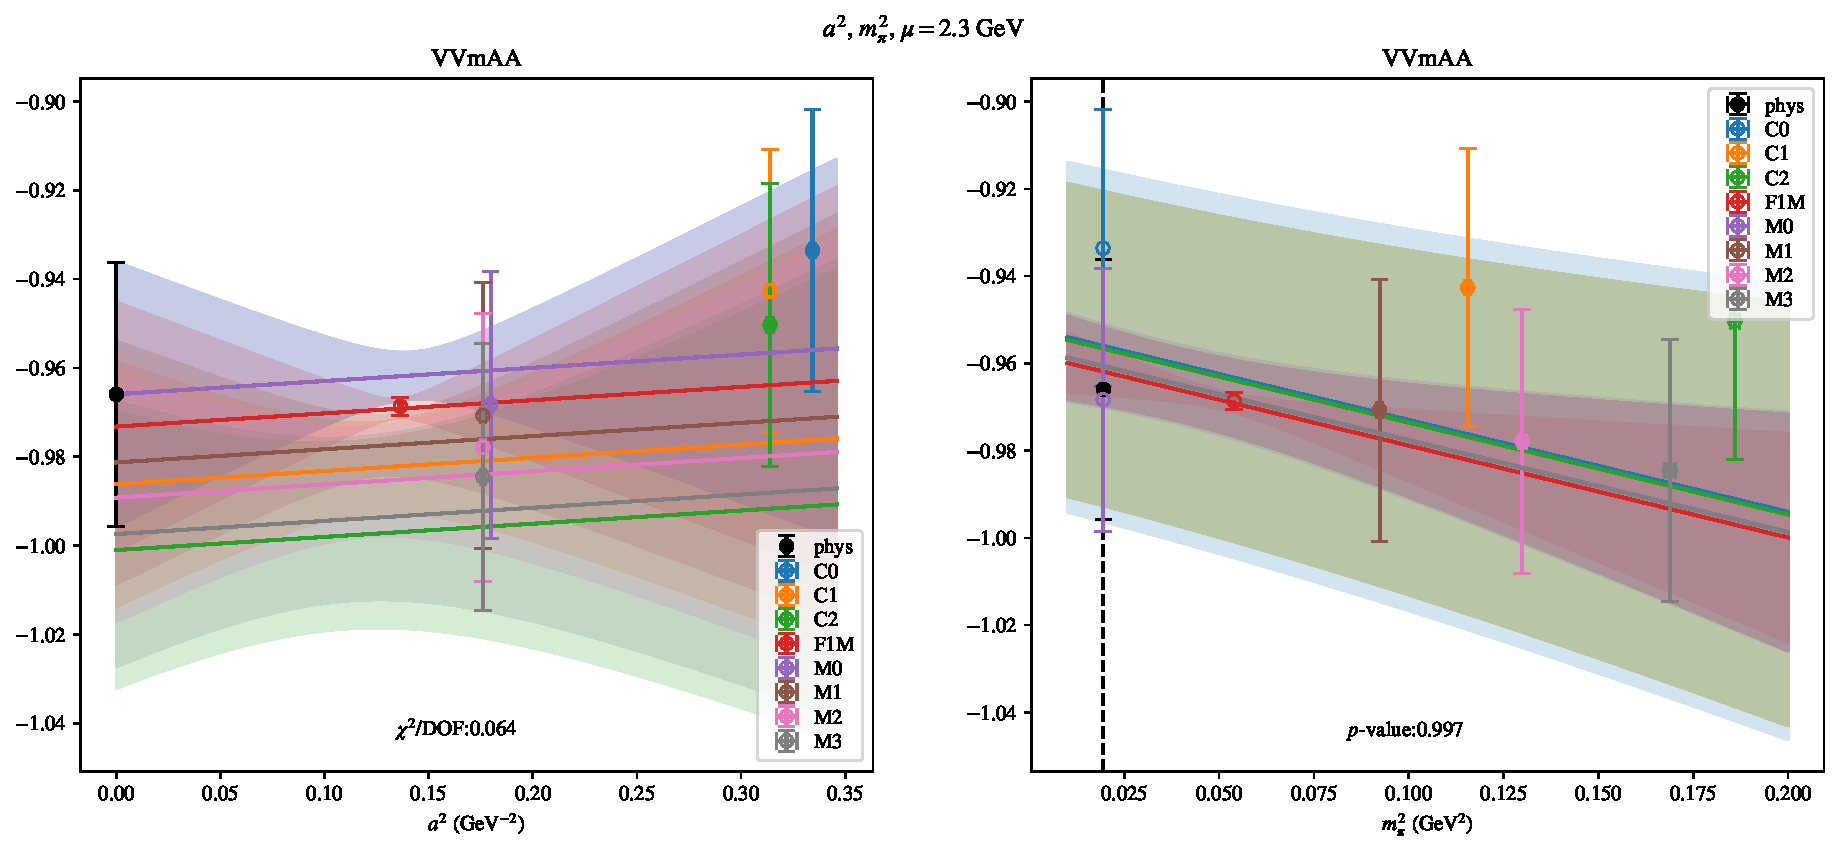
\includepdf[link, pages=-]{VVmAA/NPR/a2m2_23.pdf}
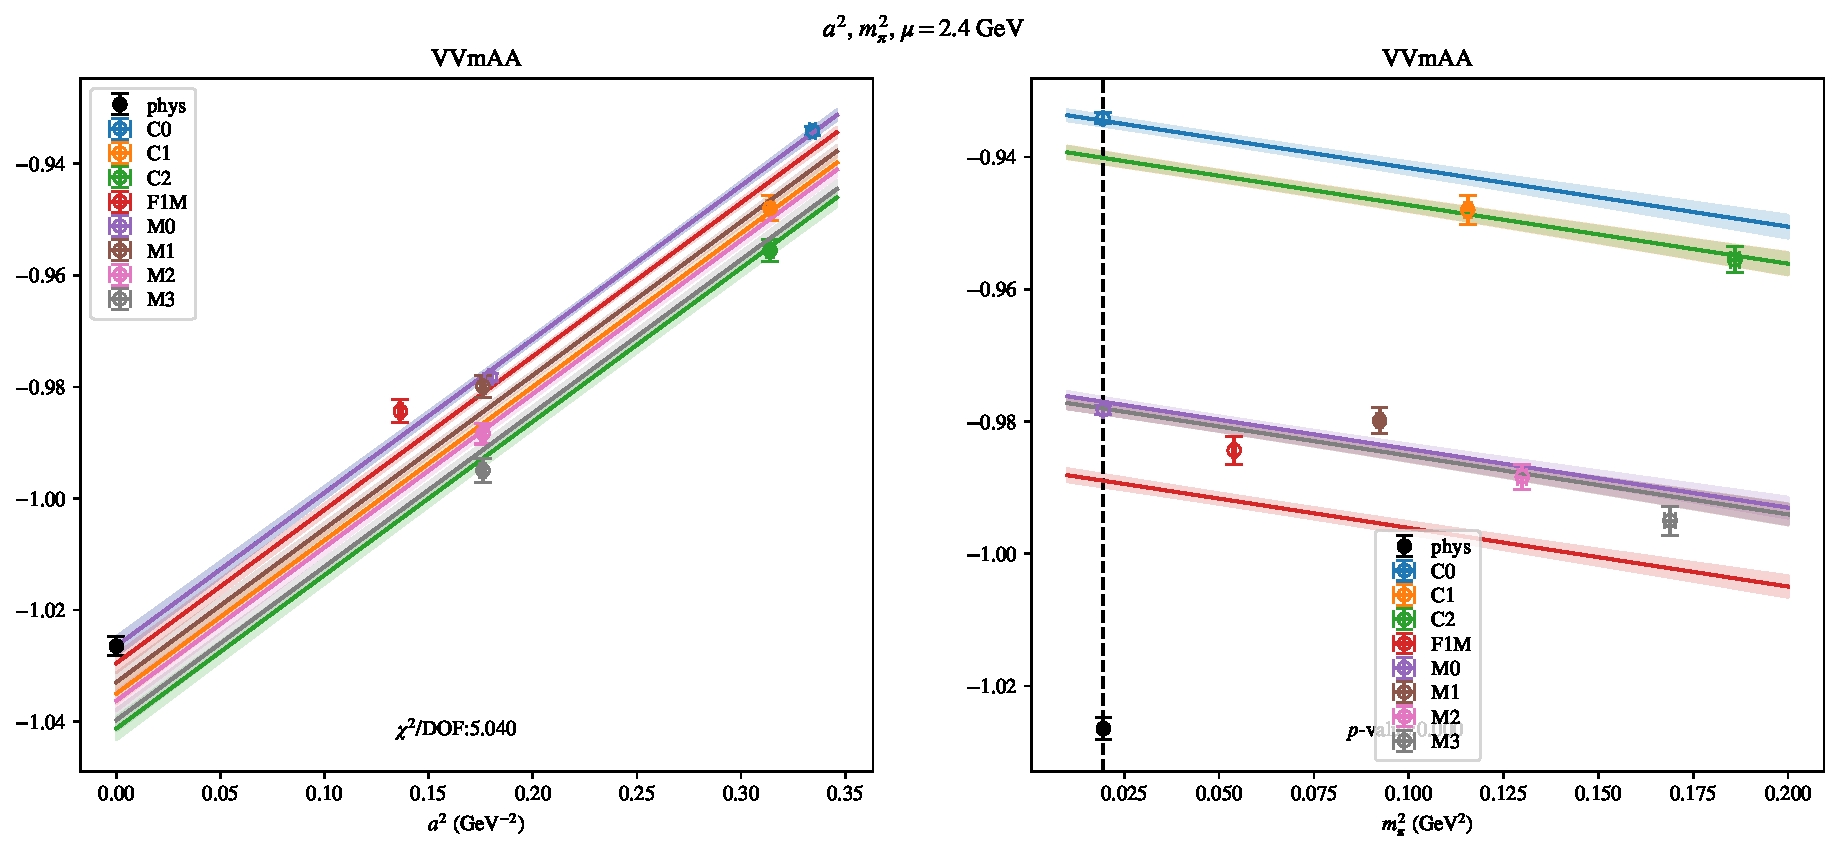
\includepdf[link, pages=-]{VVmAA/NPR/a2m2_24.pdf}
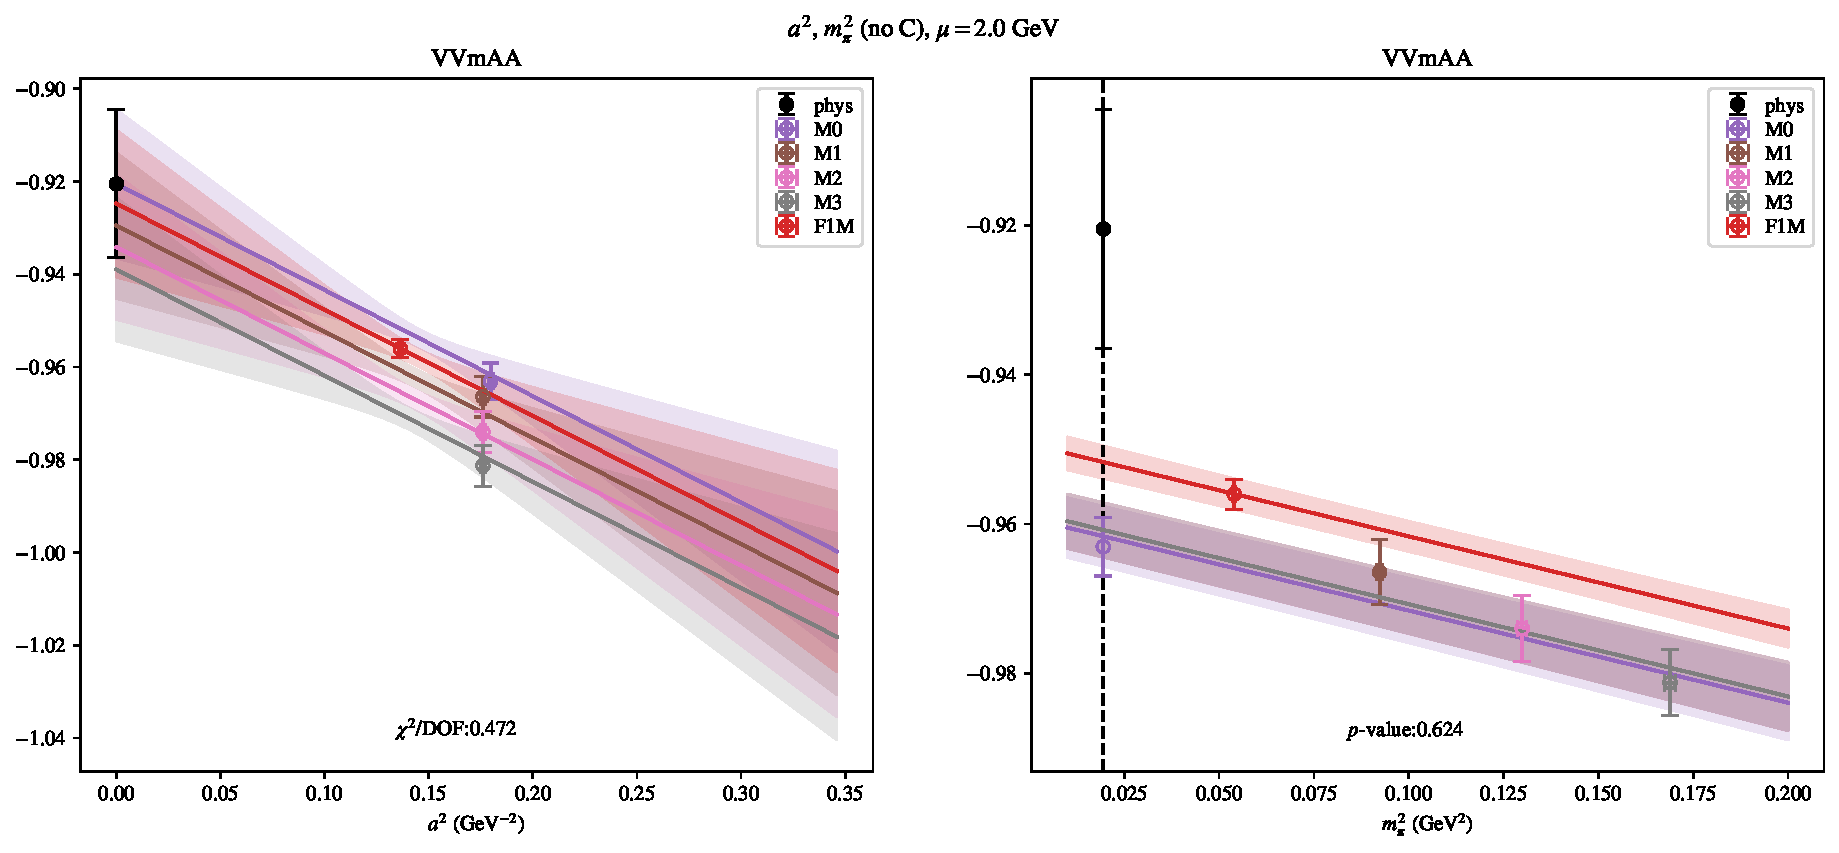
\includepdf[link, pages=-]{VVmAA/NPR/a2m2noC_20.pdf}
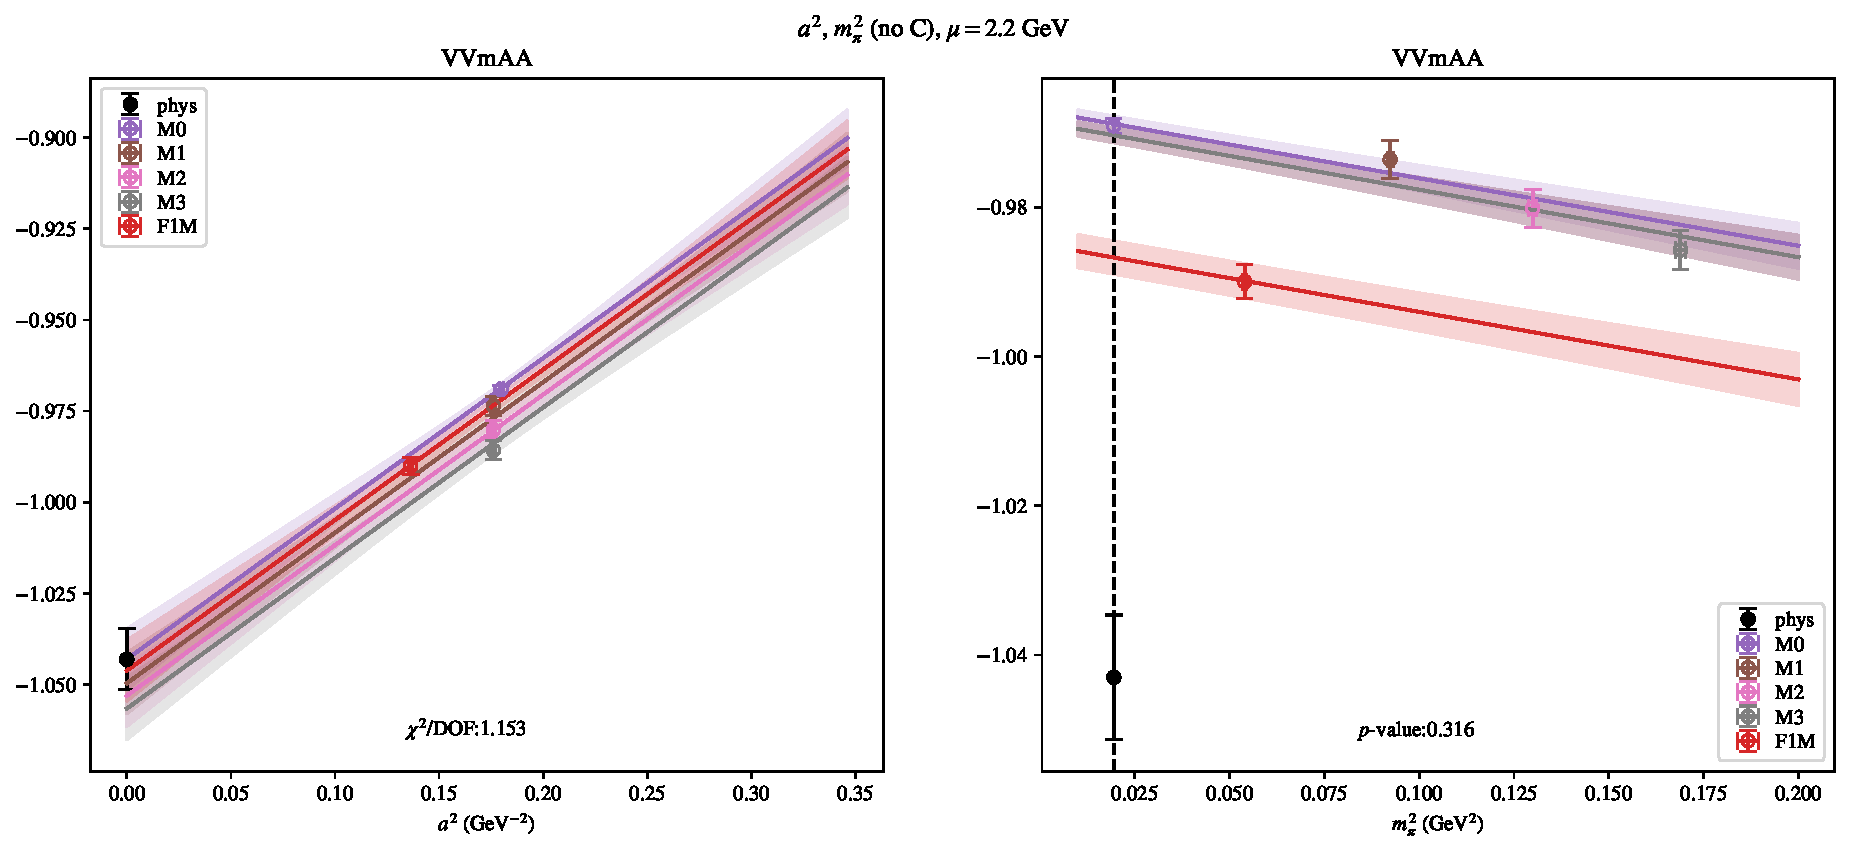
\includepdf[link, pages=-]{VVmAA/NPR/a2m2noC_22.pdf}
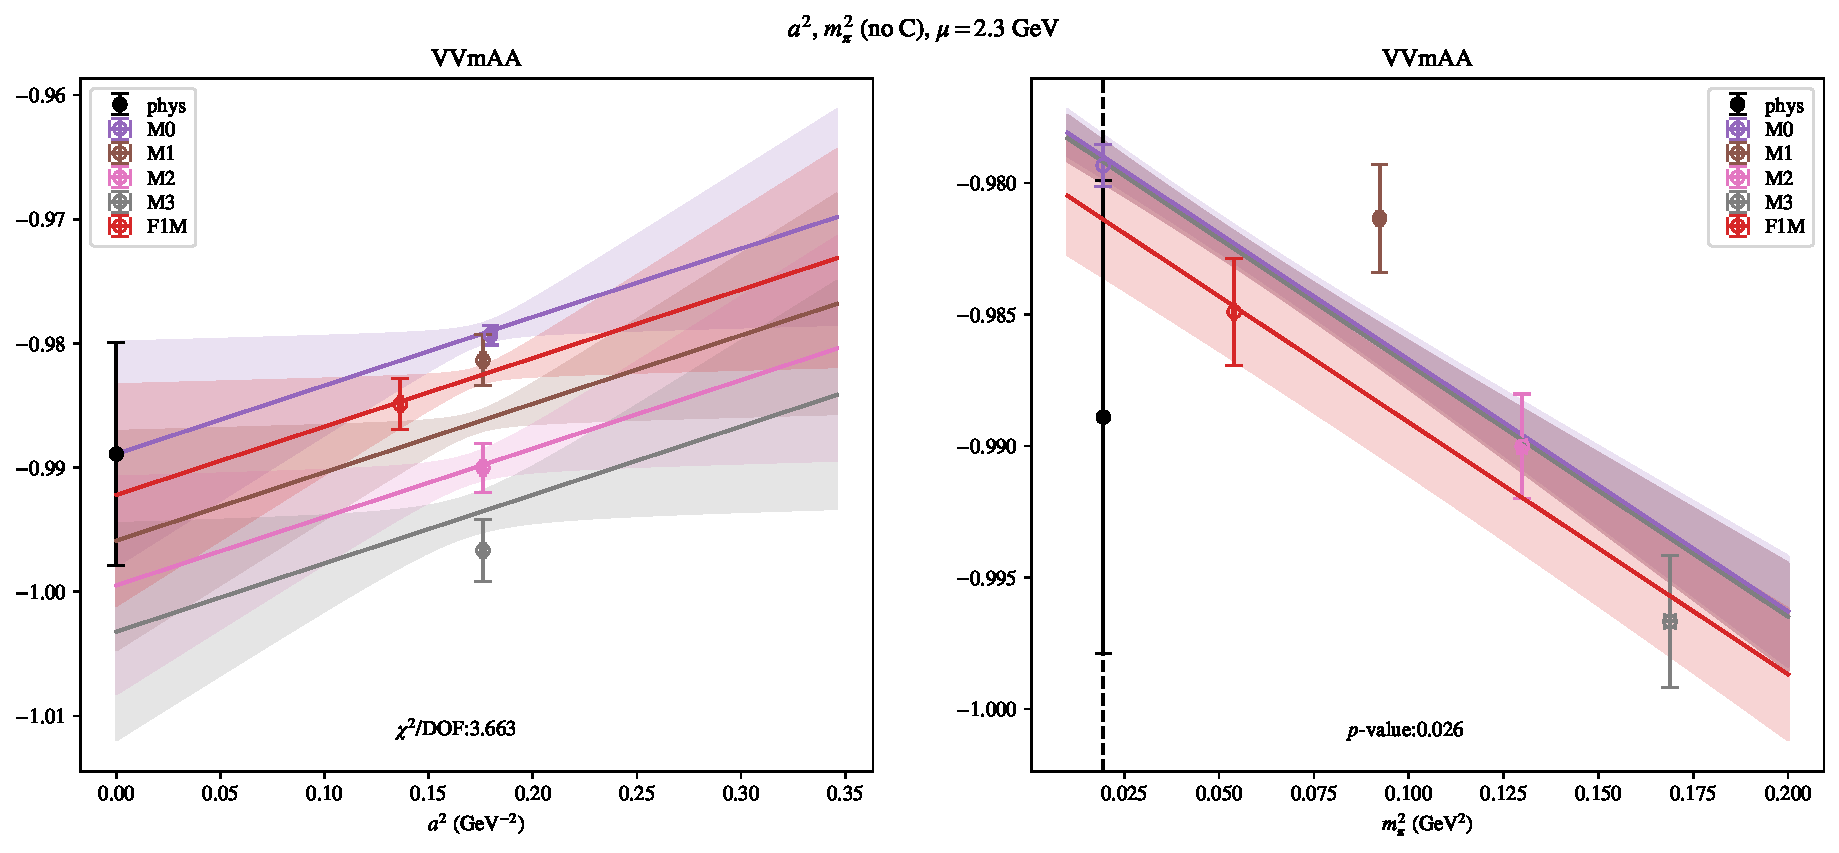
\includepdf[link, pages=-]{VVmAA/NPR/a2m2noC_23.pdf}
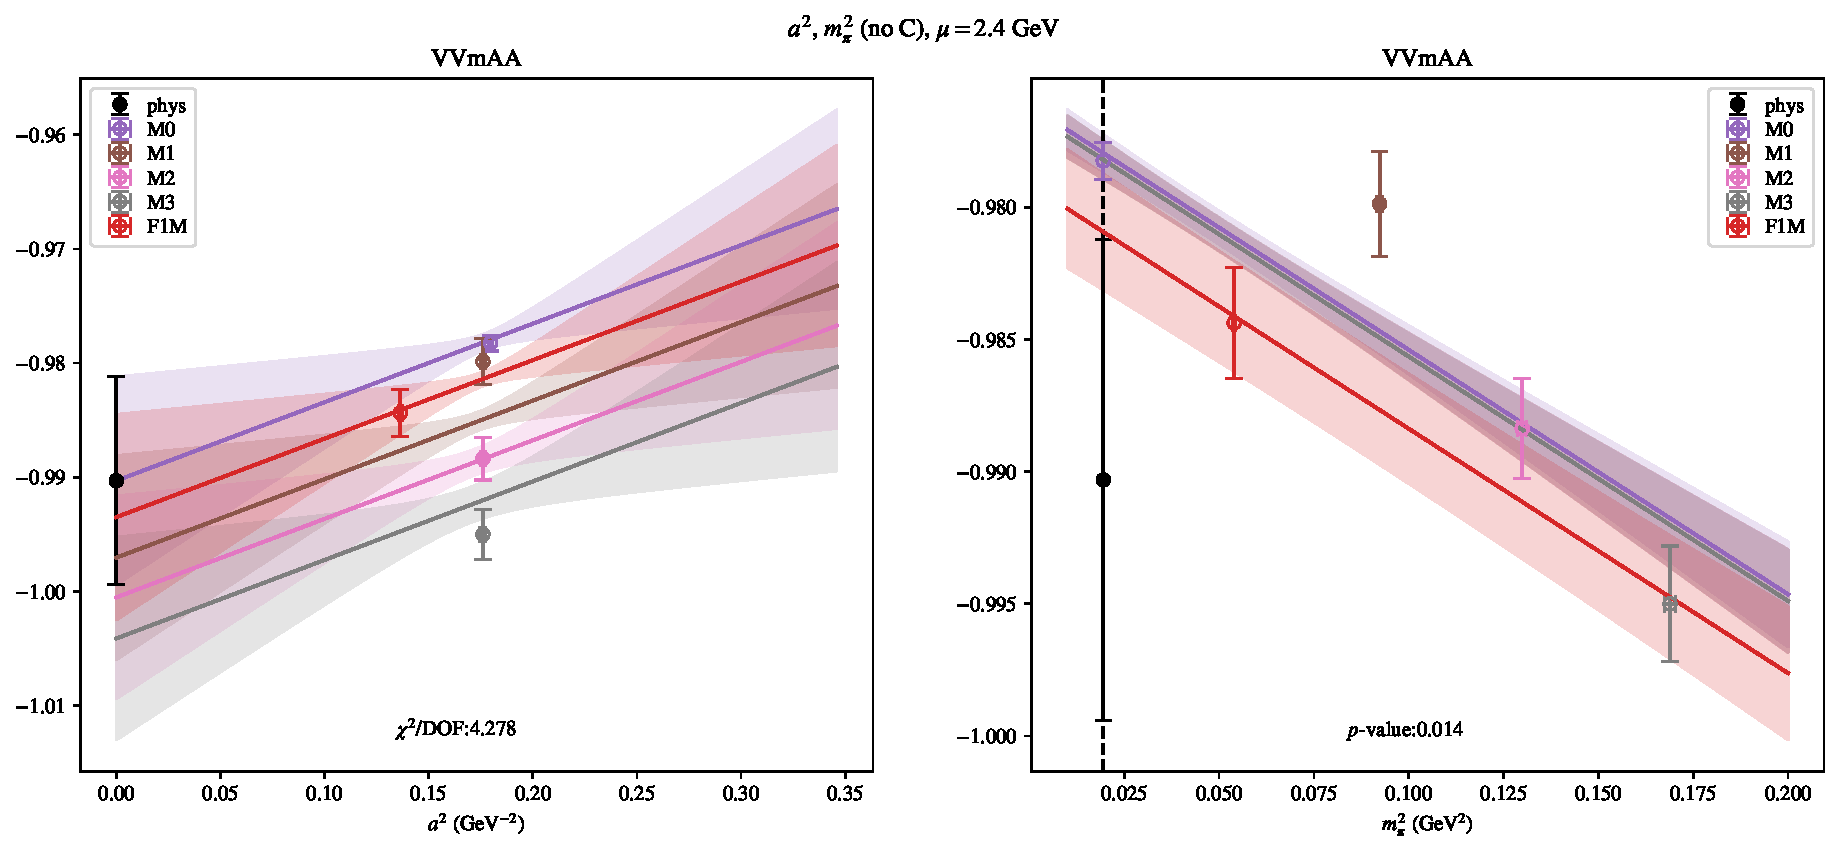
\includepdf[link, pages=-]{VVmAA/NPR/a2m2noC_24.pdf}
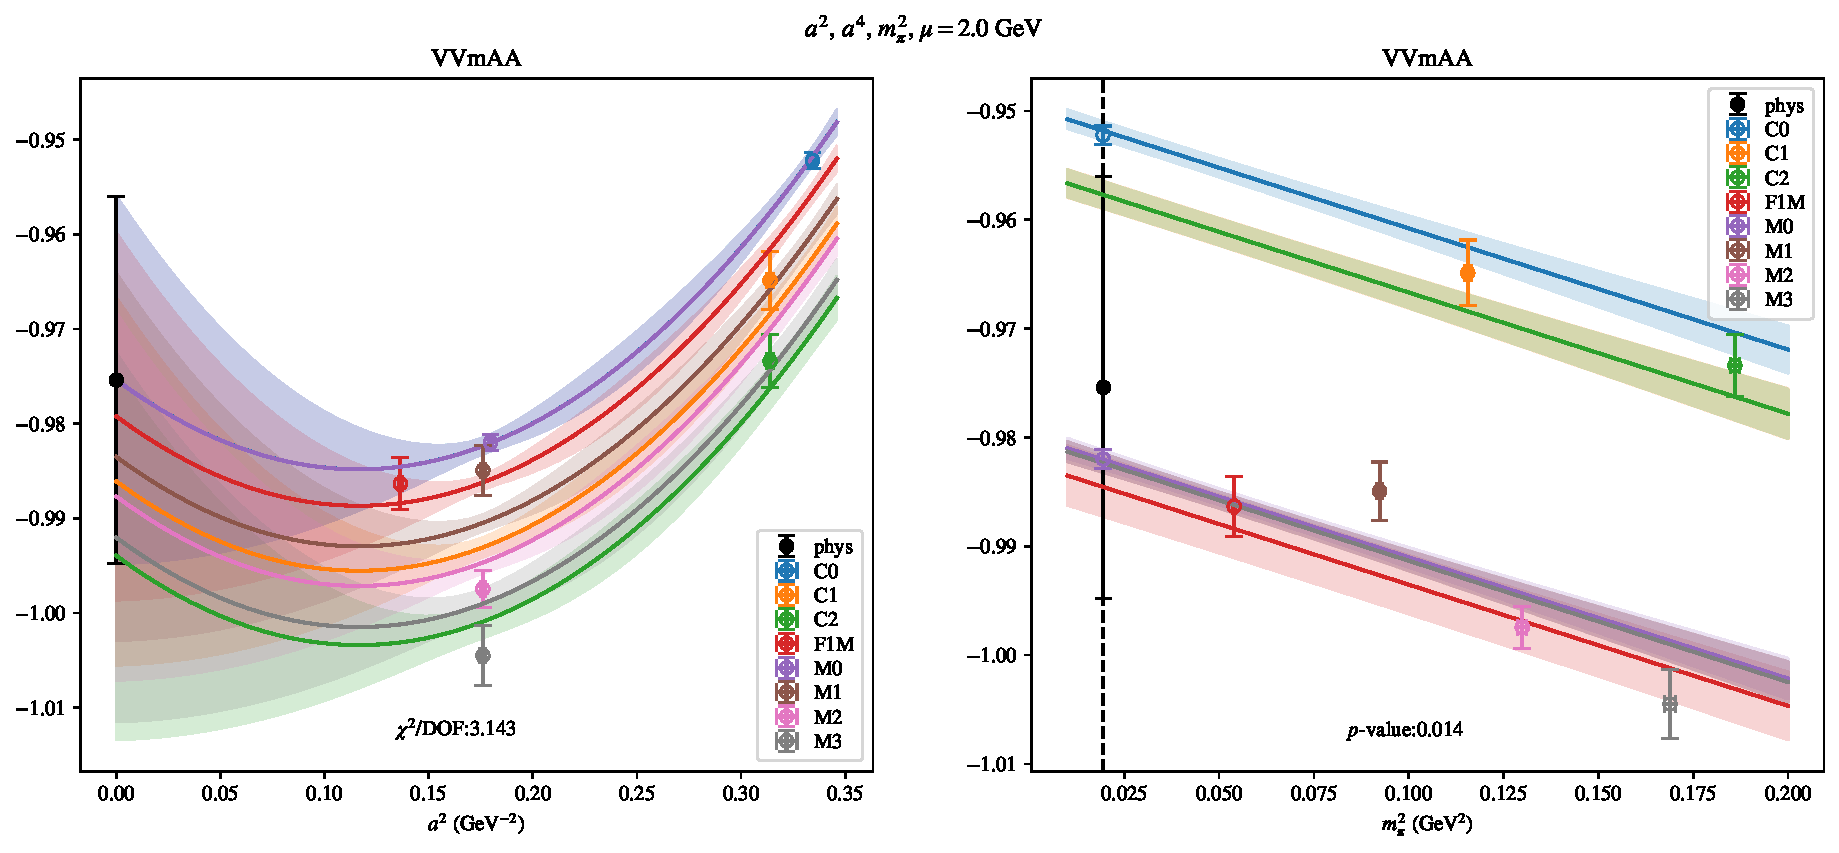
\includepdf[link, pages=-]{VVmAA/NPR/a2a4m2_20.pdf}
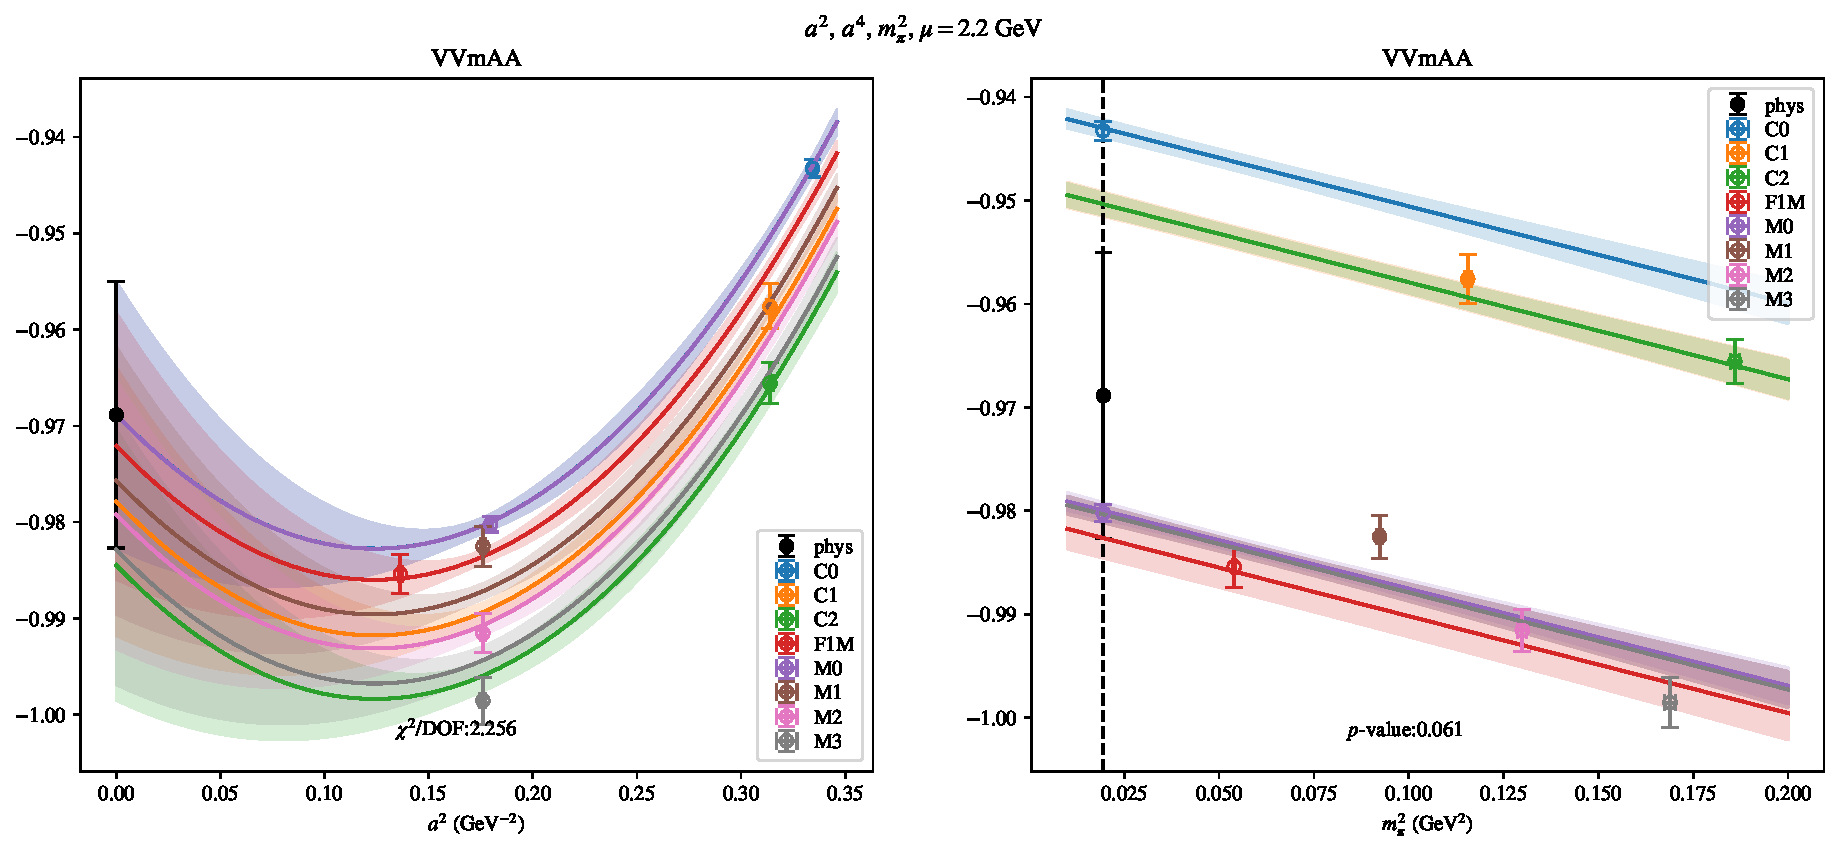
\includepdf[link, pages=-]{VVmAA/NPR/a2a4m2_22.pdf}
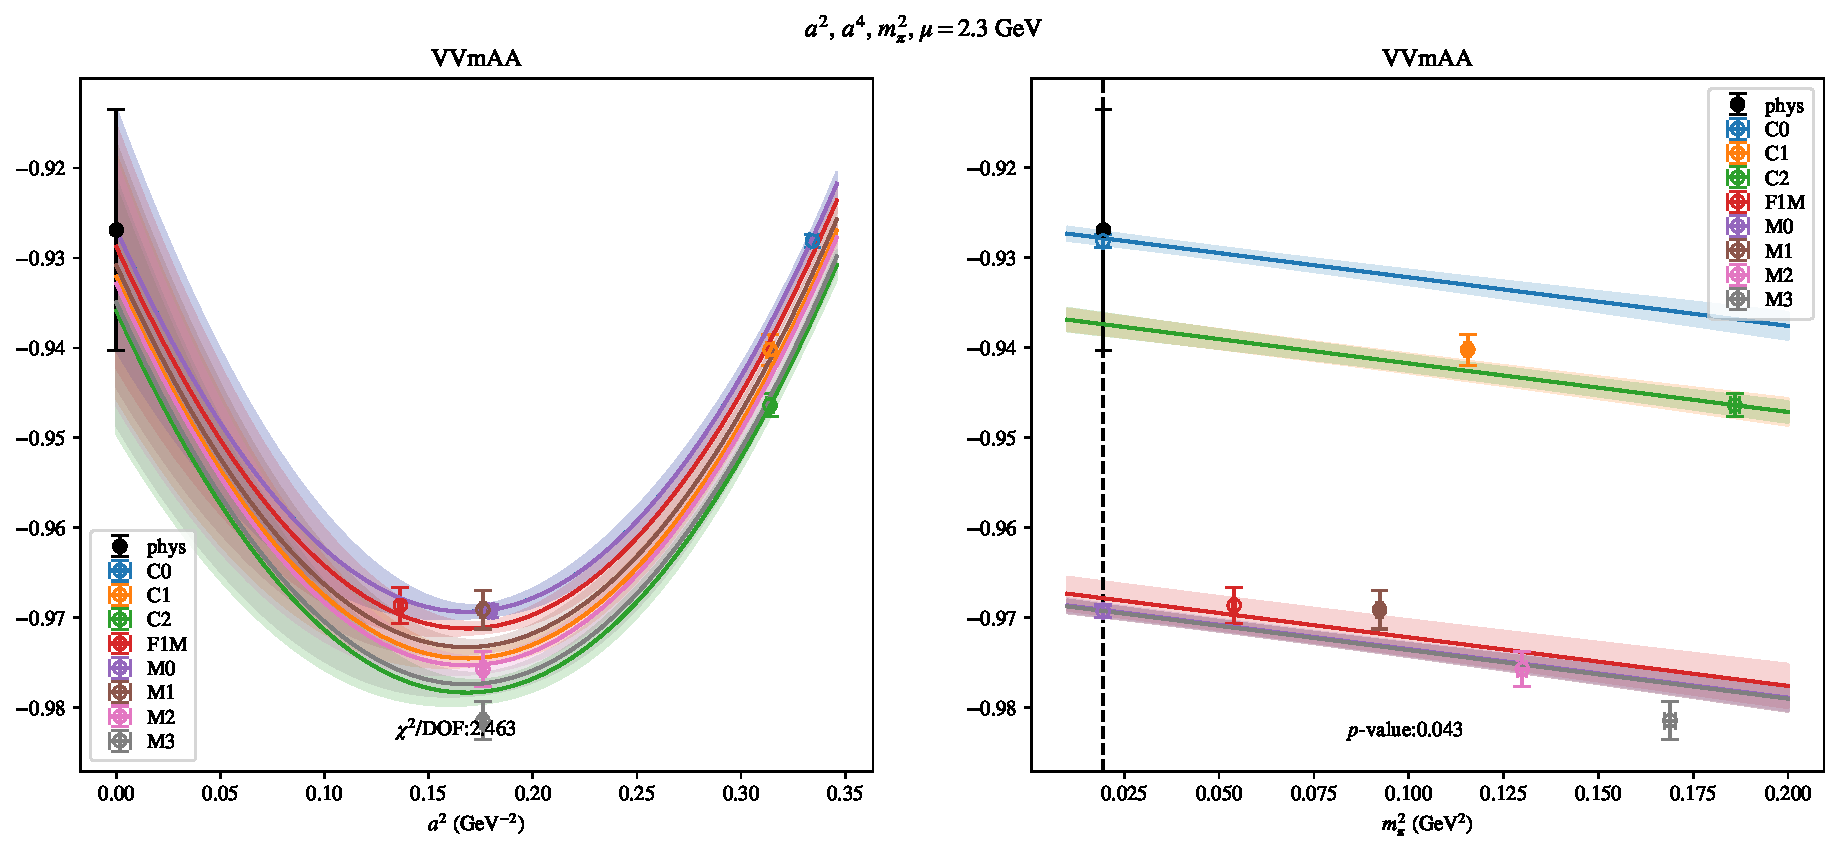
\includepdf[link, pages=-]{VVmAA/NPR/a2a4m2_23.pdf}
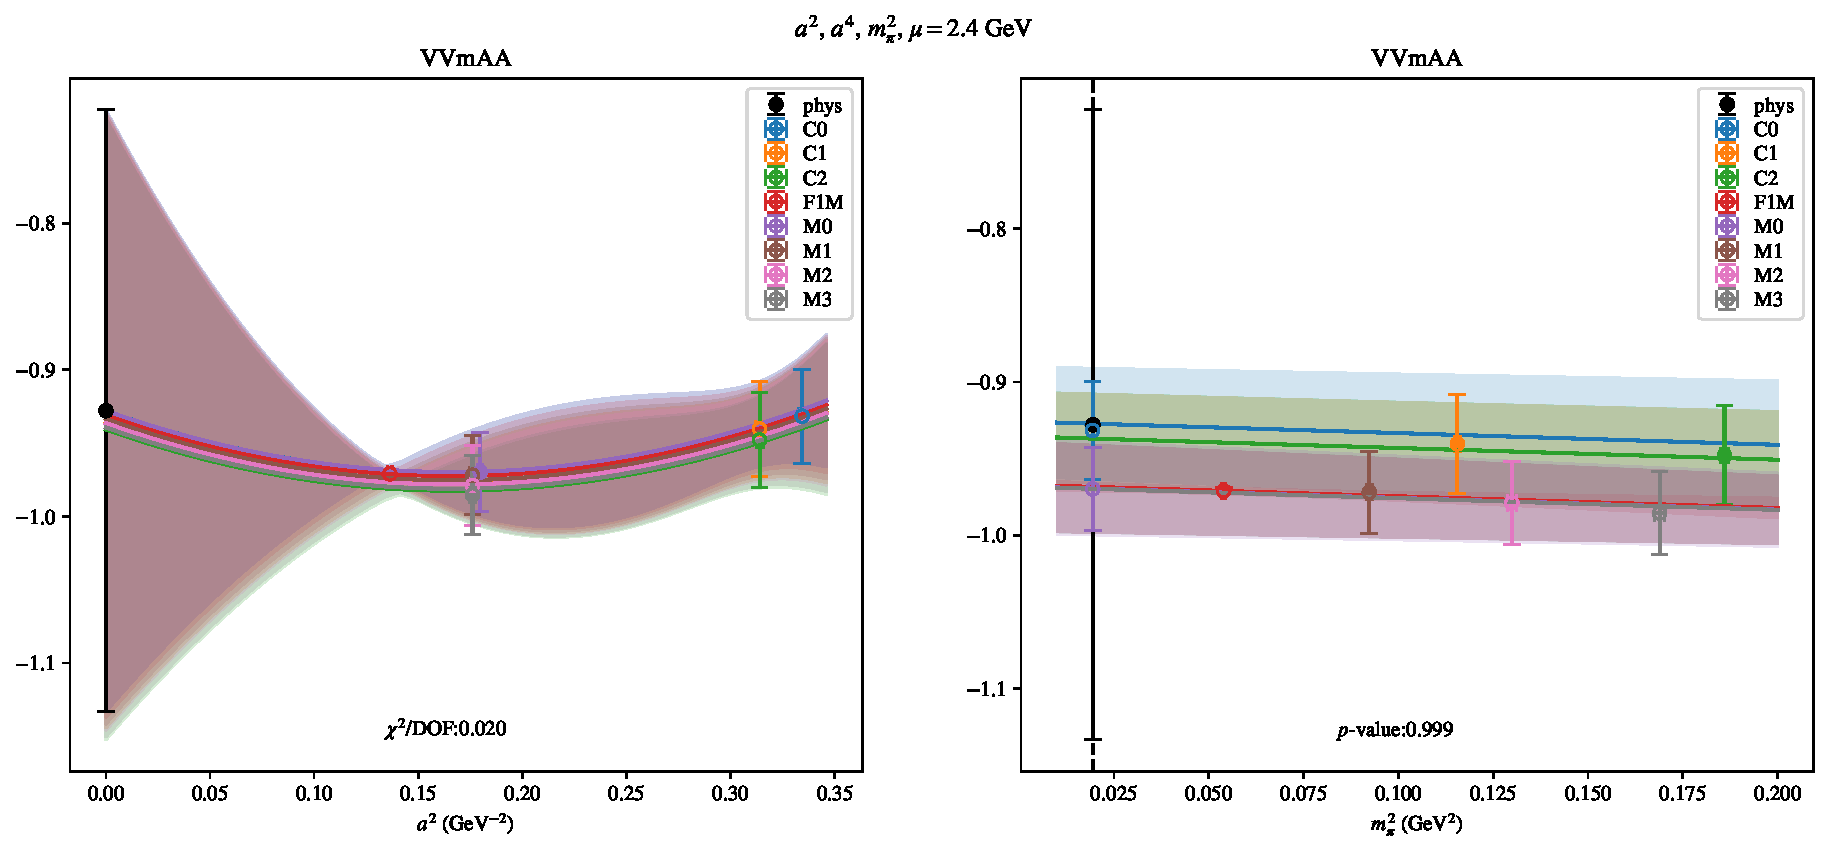
\includepdf[link, pages=-]{VVmAA/NPR/a2a4m2_24.pdf}
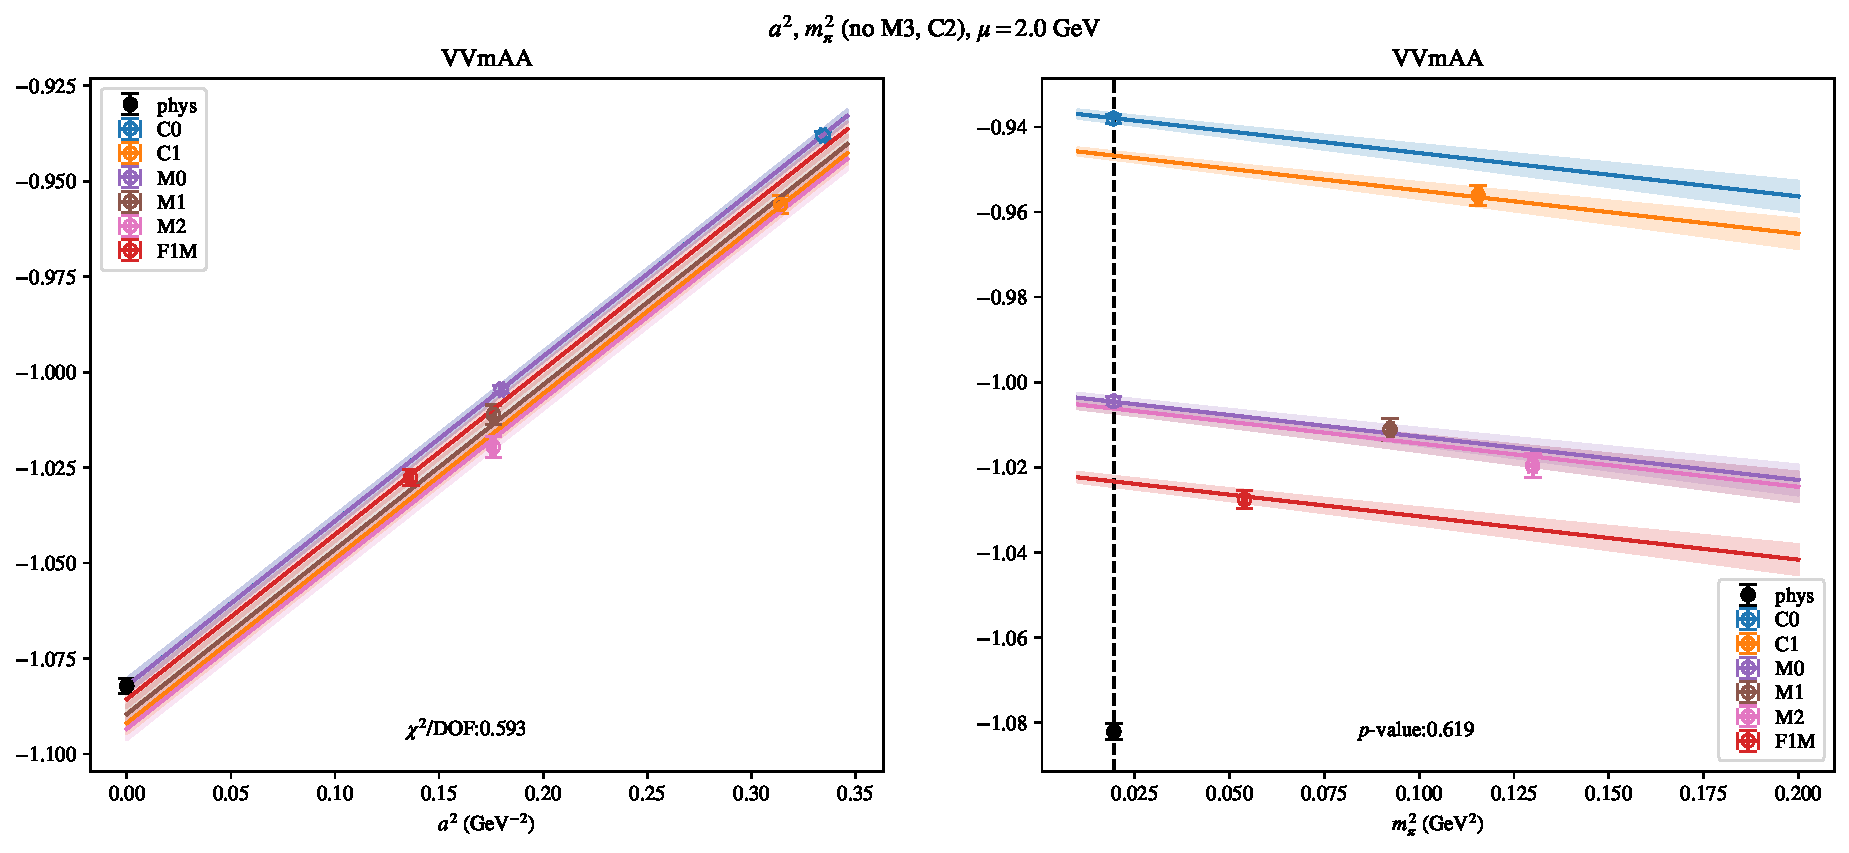
\includepdf[link, pages=-]{VVmAA/NPR/a2m2mcut_20.pdf}
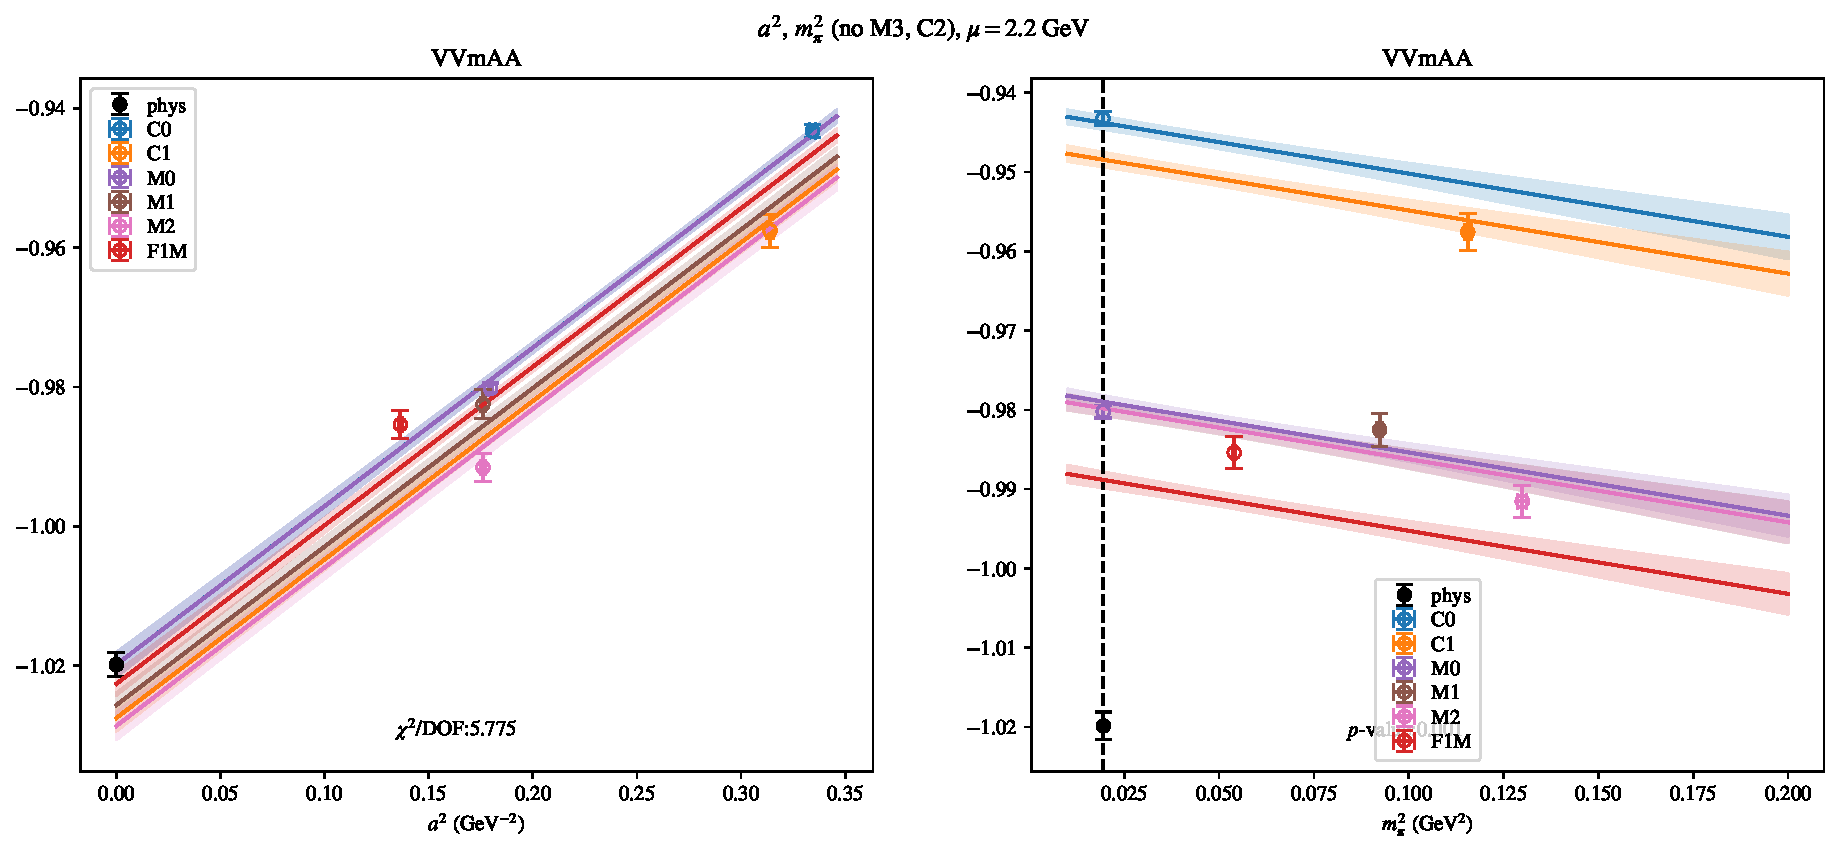
\includepdf[link, pages=-]{VVmAA/NPR/a2m2mcut_22.pdf}
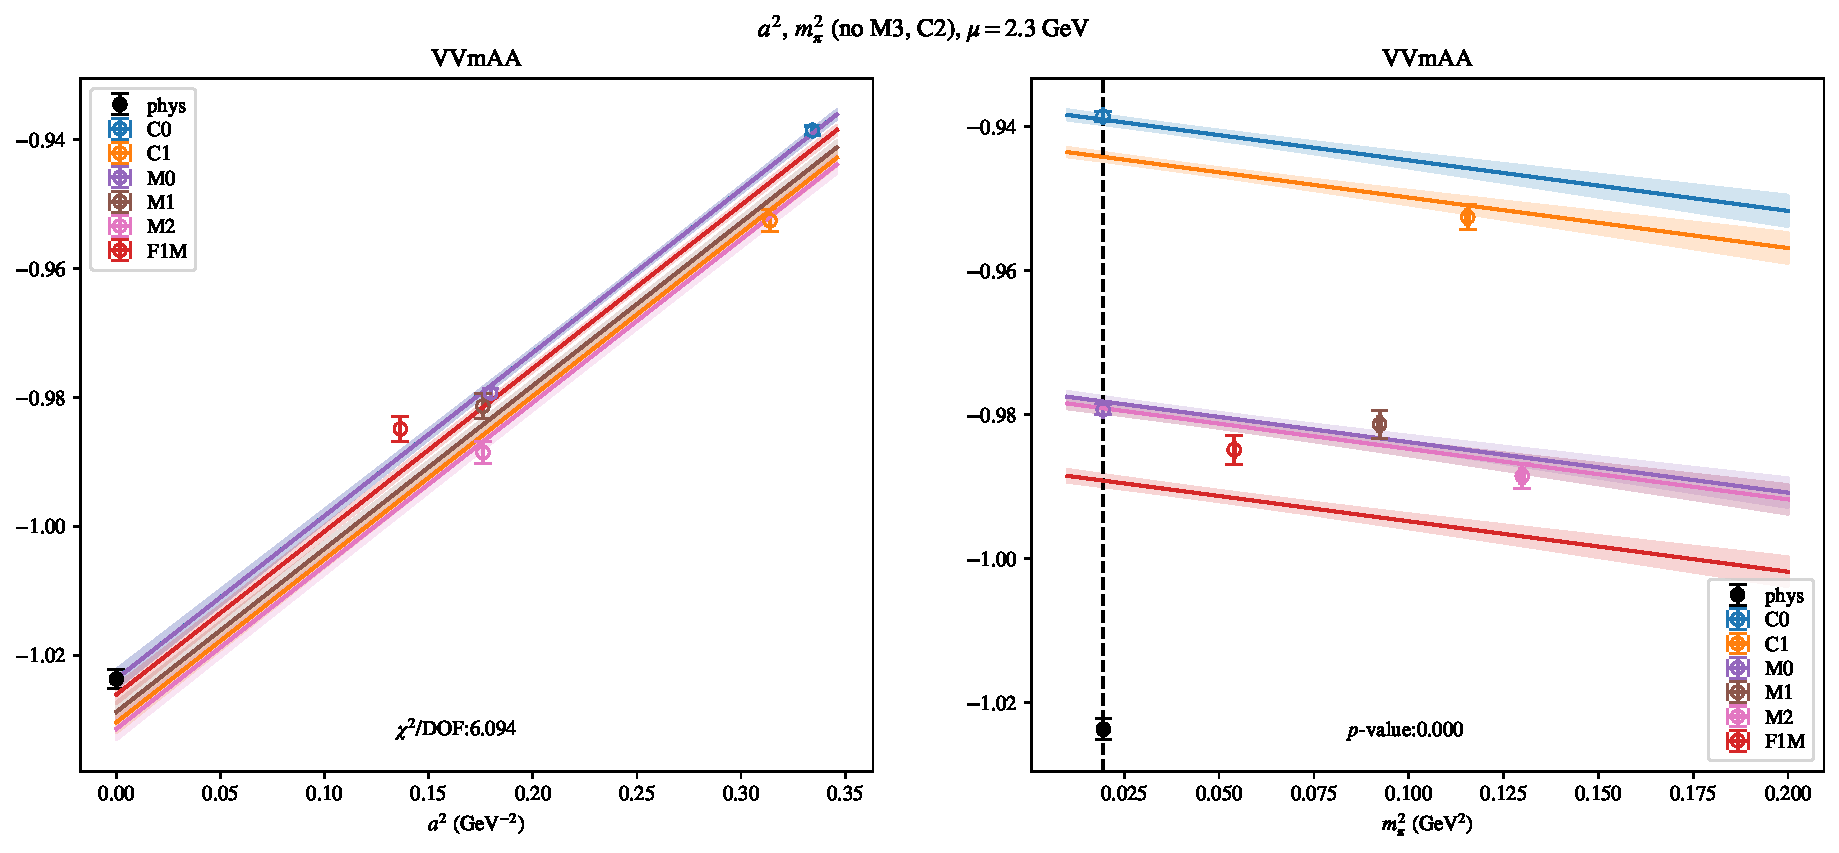
\includepdf[link, pages=-]{VVmAA/NPR/a2m2mcut_23.pdf}
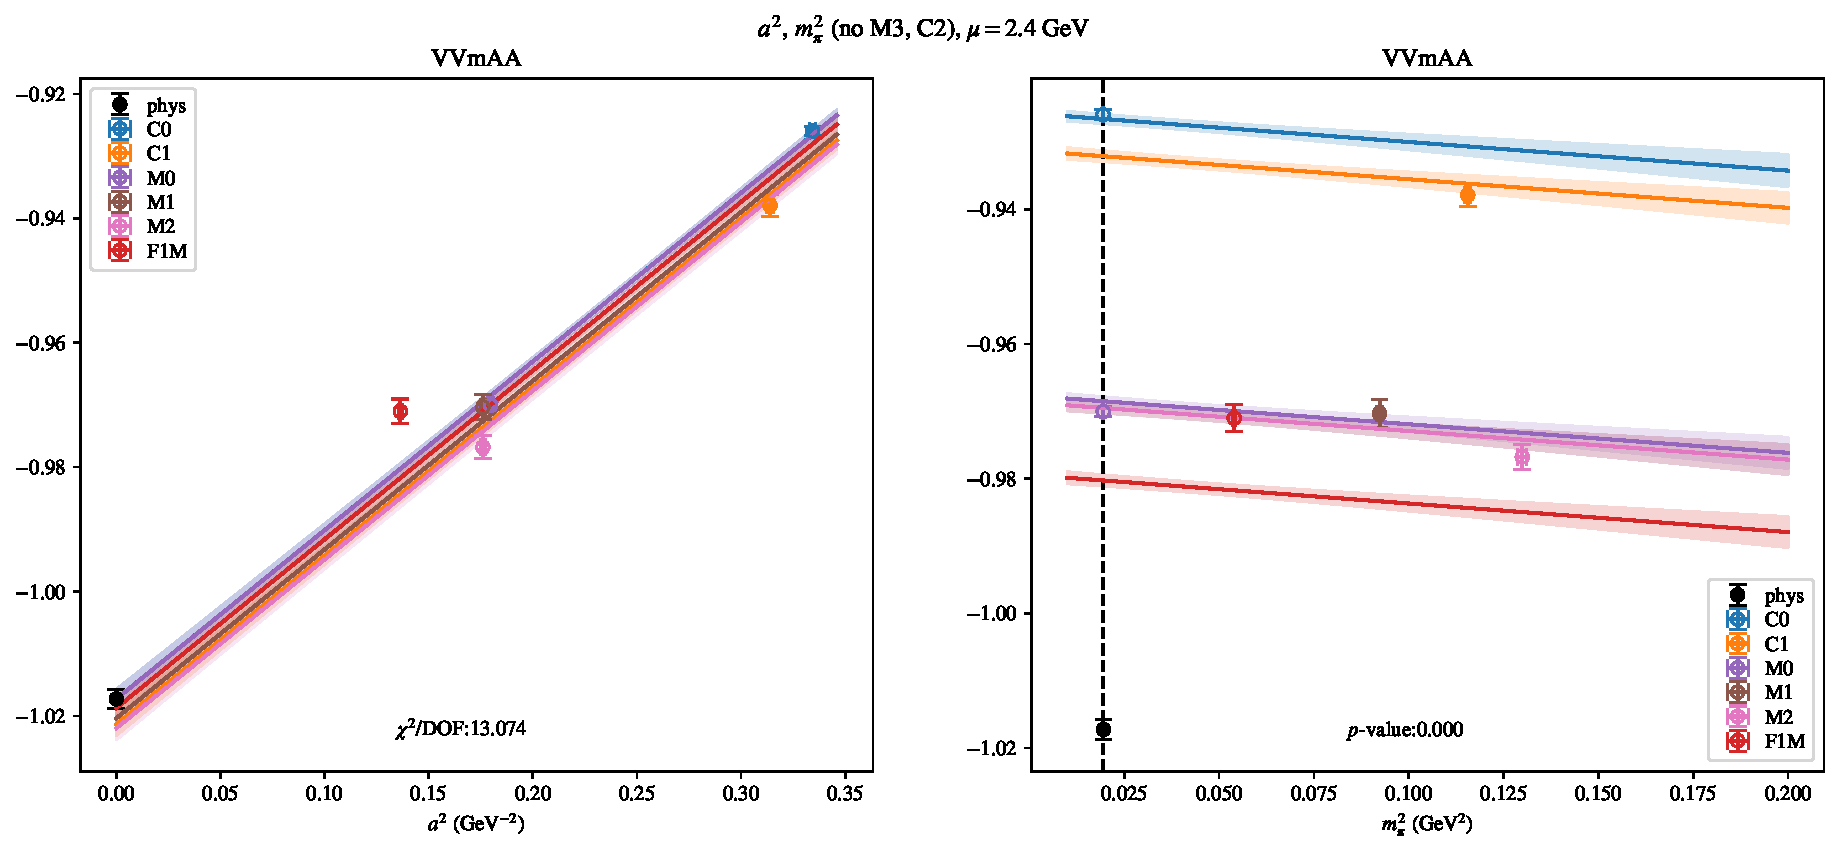
\includepdf[link, pages=-]{VVmAA/NPR/a2m2mcut_24.pdf}
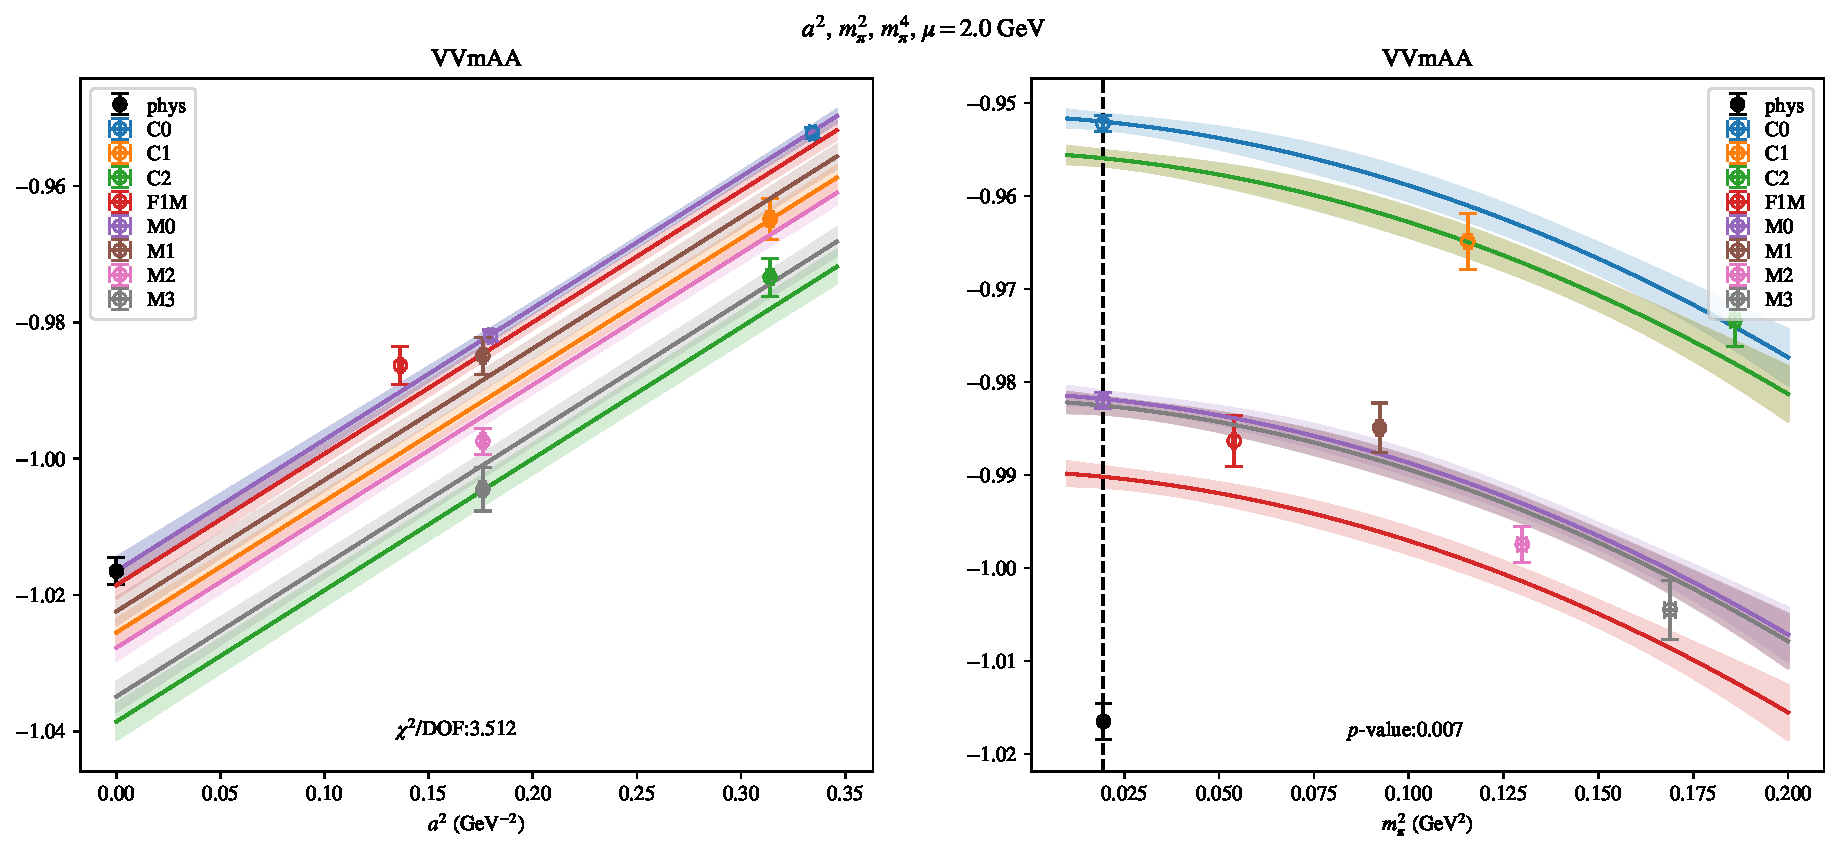
\includepdf[link, pages=-]{VVmAA/NPR/a2m2m4_20.pdf}
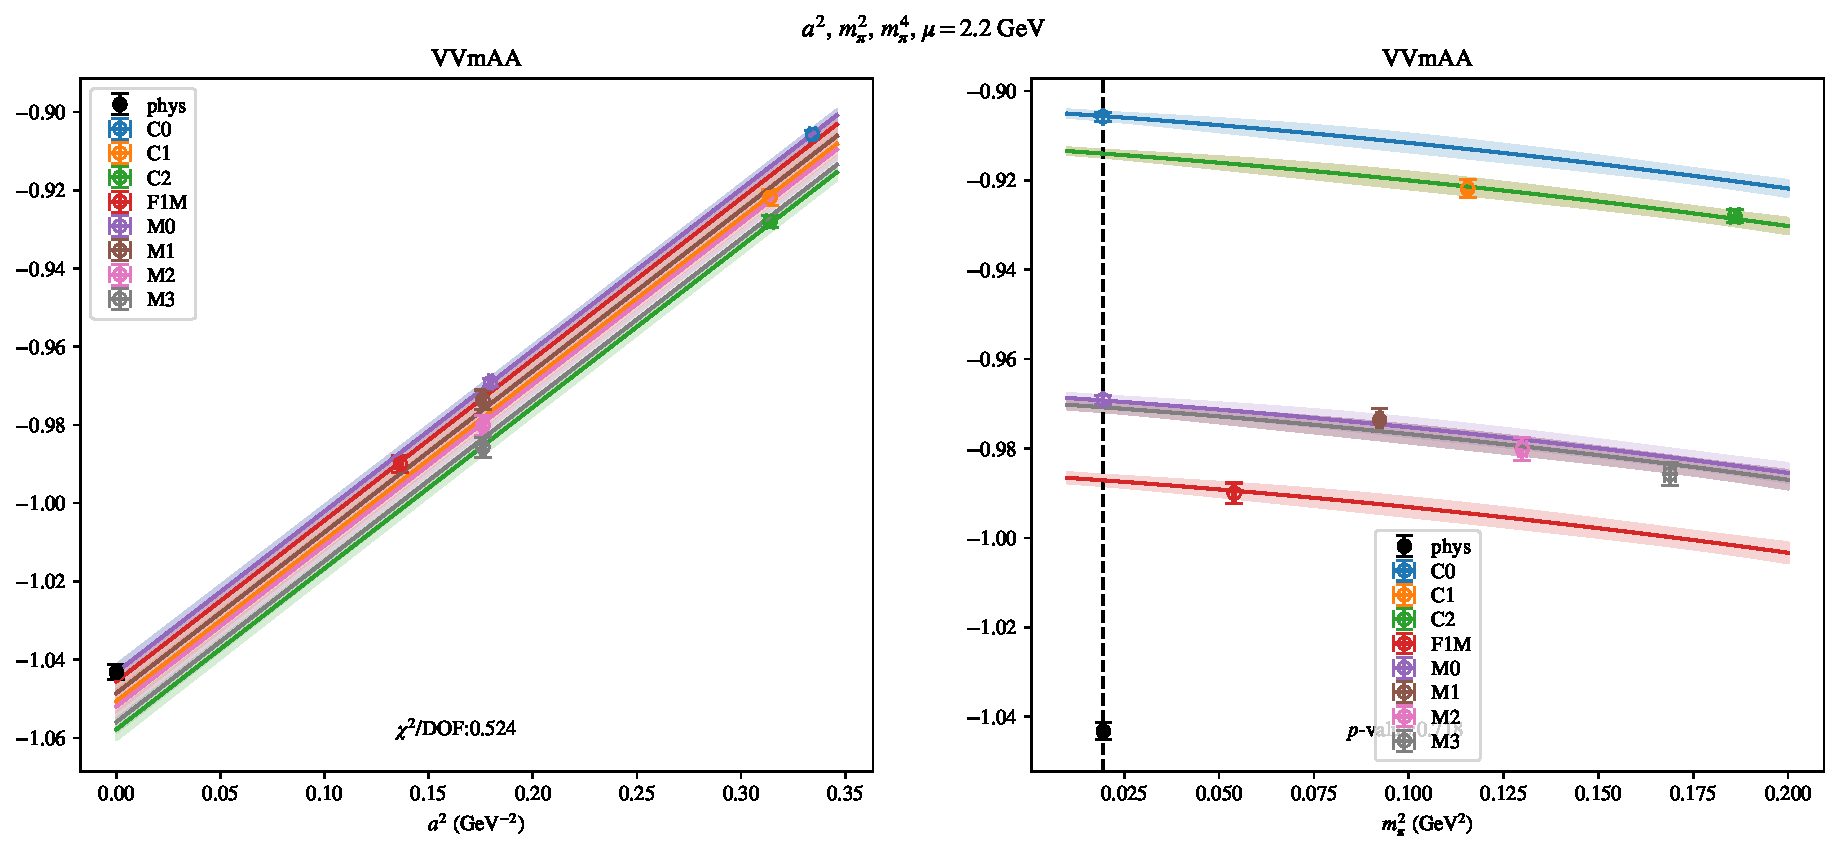
\includepdf[link, pages=-]{VVmAA/NPR/a2m2m4_22.pdf}
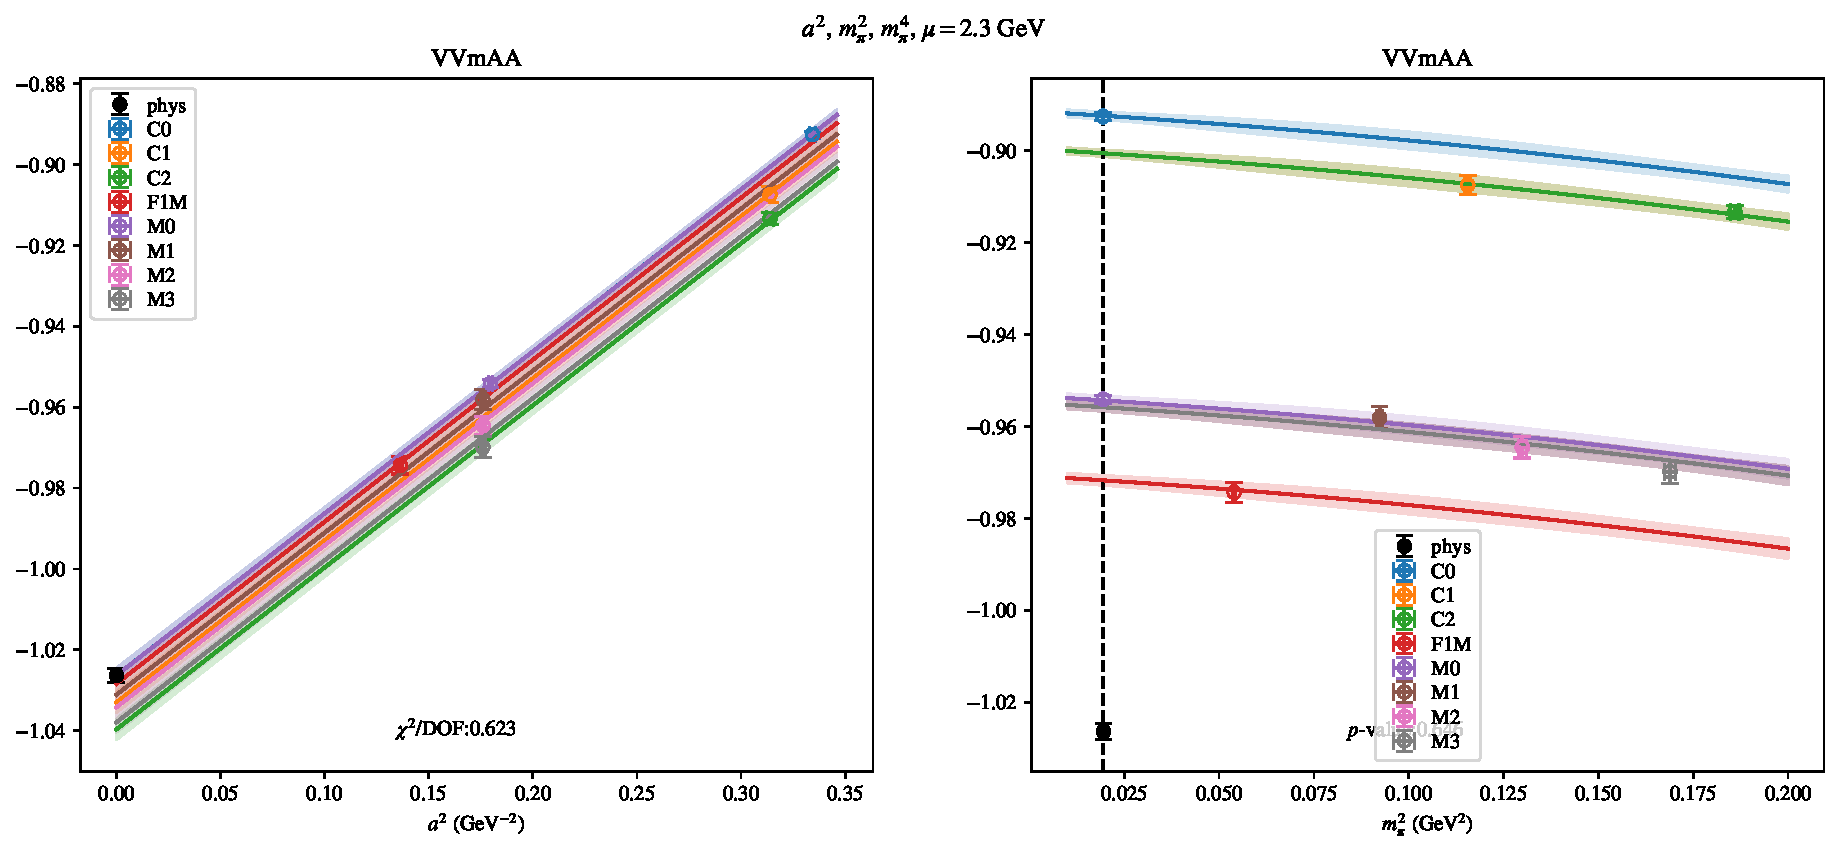
\includepdf[link, pages=-]{VVmAA/NPR/a2m2m4_23.pdf}
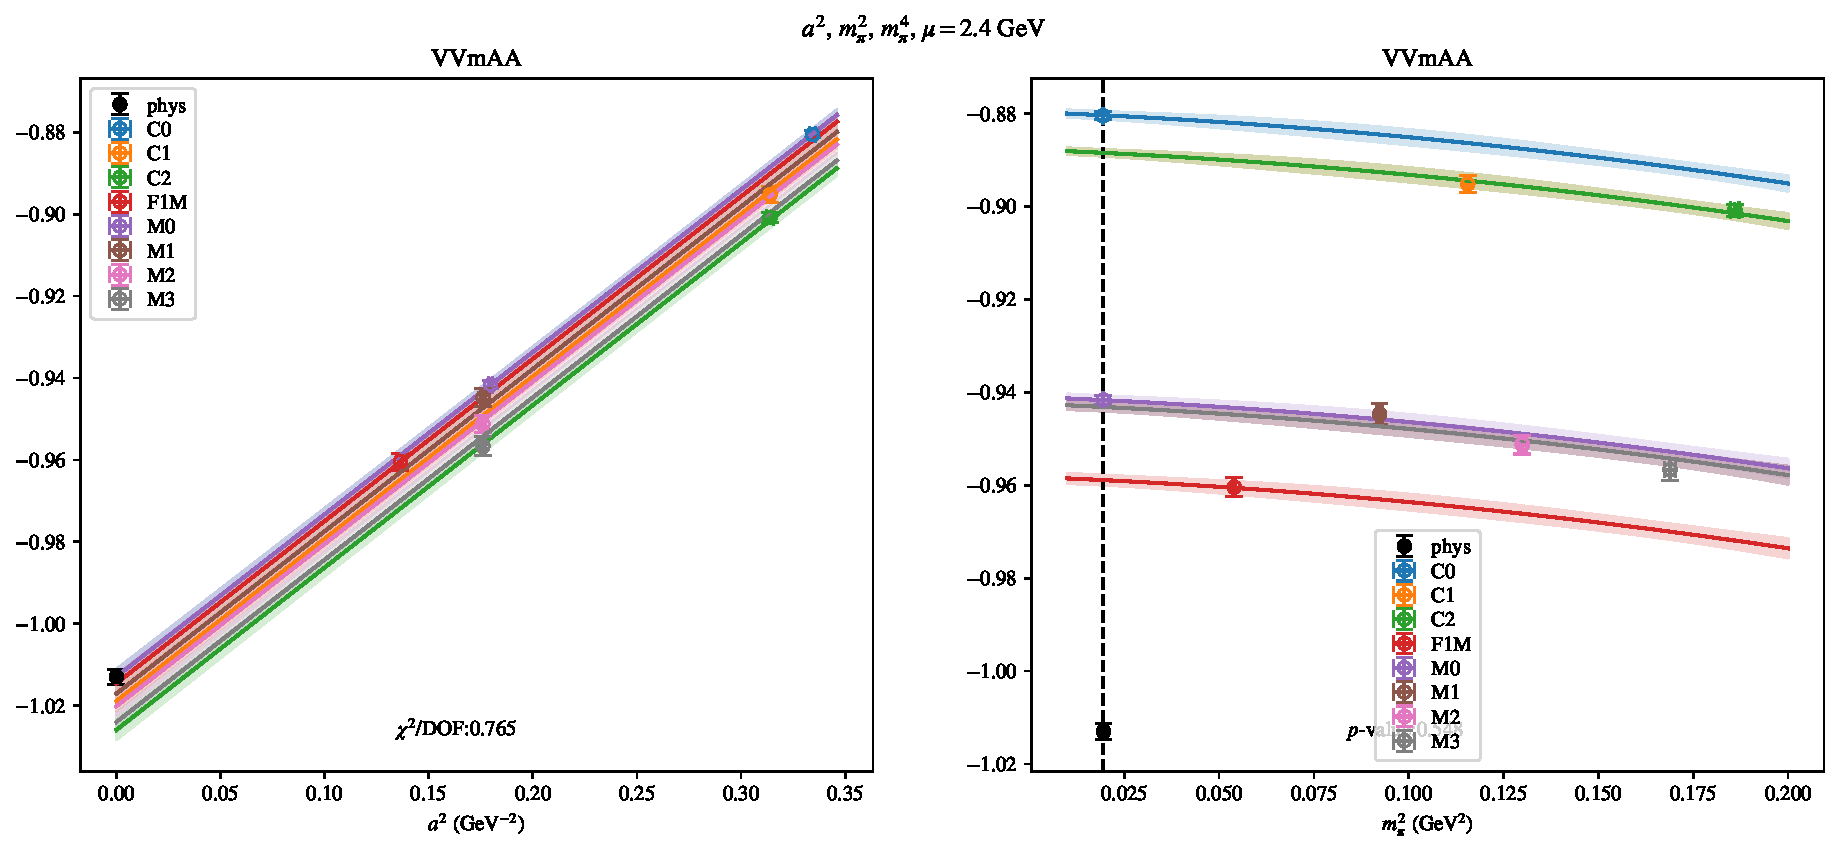
\includepdf[link, pages=-]{VVmAA/NPR/a2m2m4_24.pdf}
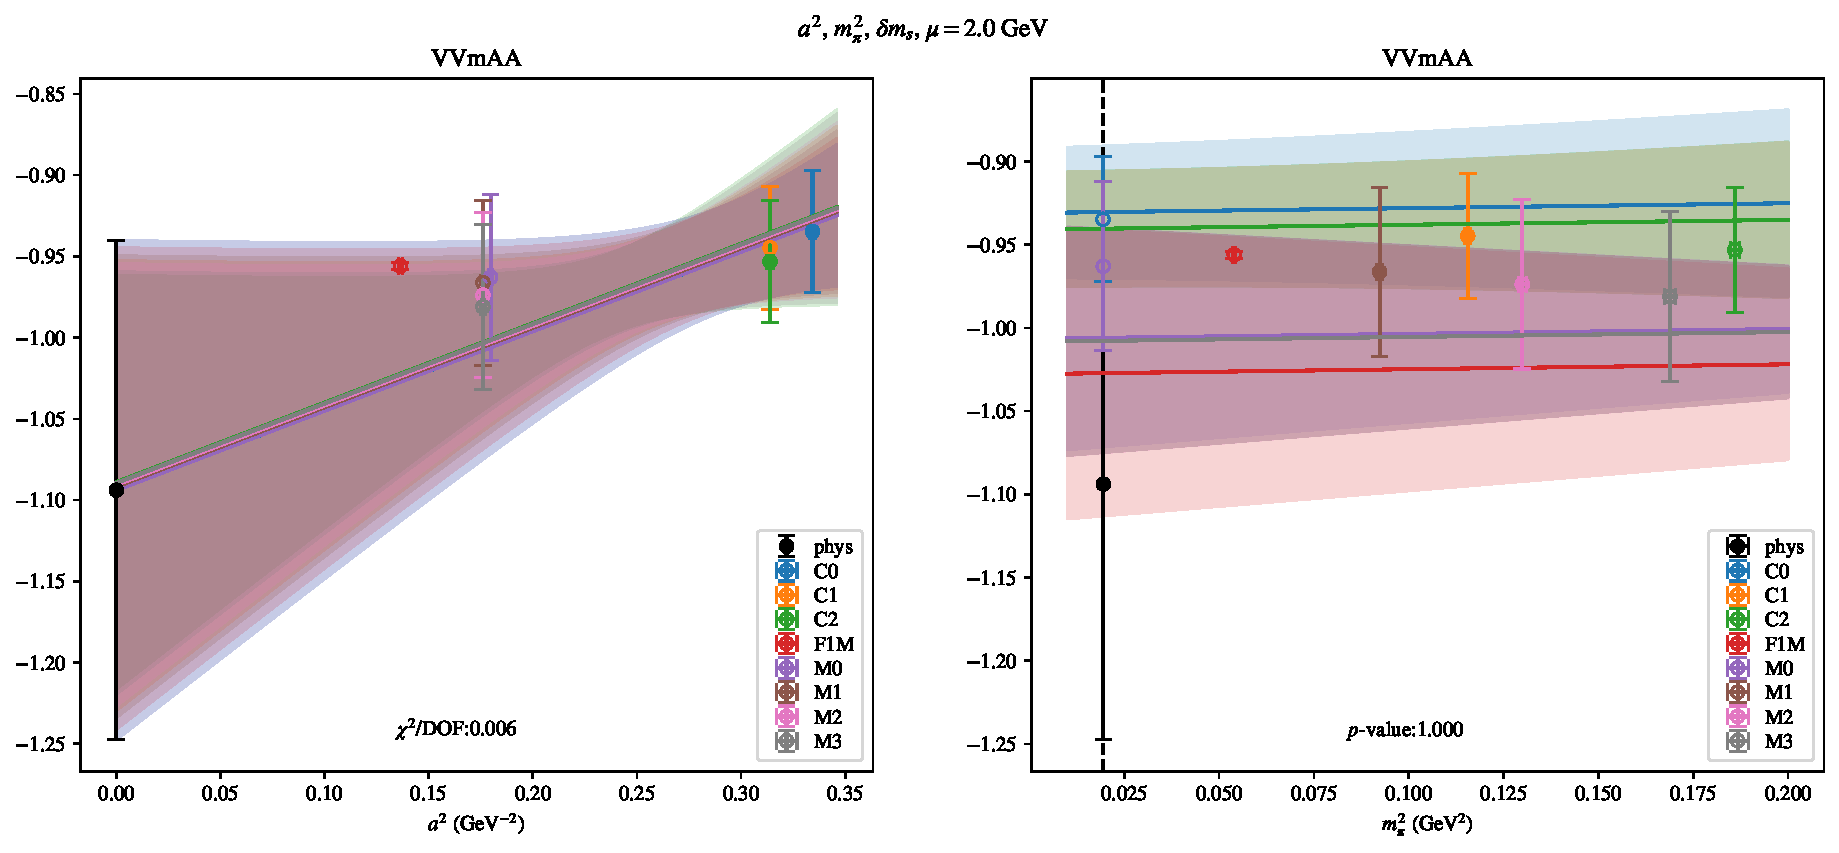
\includepdf[link, pages=-]{VVmAA/NPR/a2m2delm_20.pdf}
\includepdf[link, pages=-]{VVmAA/NPR/a2m2delm_22.pdf}
\includepdf[link, pages=-]{VVmAA/NPR/a2m2delm_23.pdf}
\includepdf[link, pages=-]{VVmAA/NPR/a2m2delm_24.pdf}
\clearpage
\section{$\mathcal{B}_3$}
\begin{table}[h!]
\begin{center}
\begin{tabular}{|c|c|c|c|c|c|c|}
\hline
$\mu$ (GeV) & $a^2$, $m_\pi^2$& $a^2$, $m_\pi^2$ (no C)& $a^2$, $a^4$, $m_\pi^2$& $a^2$, $m_\pi^2$ (no M3, C2)& $a^2$, $m_\pi^2$, $m_\pi^4$& $a^2$, $m_\pi^2$, $\delta m_s$\\
\hline
2.0& \hyperlink{SSmPP/NPR/a2m2_20.pdf.1}{\textbf{1.7994(28)}: 19.68 (0.0)} & \hyperlink{SSmPP/NPR/a2m2noC_20.pdf.1}{\textbf{1.672(15)}: 0.134 (0.874)} & \hyperlink{SSmPP/NPR/a2a4m2_20.pdf.1}{\textbf{1.596(22)}: 1.119 (0.346)} & \hyperlink{SSmPP/NPR/a2m2mcut_20.pdf.1}{\textbf{1.8014(29)}: 28.66 (0.0)} & \hyperlink{SSmPP/NPR/a2m2m4_20.pdf.1}{\textbf{1.8074(29)}: 14.12 (0.0)} & \hyperlink{SSmPP/NPR/a2m2delm_20.pdf.1}{\textbf{1.8139(31)}: 0.249 (0.91)}\\
2.2& \hyperlink{SSmPP/NPR/a2m2_22.pdf.1}{\textbf{1.8058(28)}: 16.073 (0.0)} & \hyperlink{SSmPP/NPR/a2m2noC_22.pdf.1}{\textbf{1.696(13)}: 0.638 (0.528)} & \hyperlink{SSmPP/NPR/a2a4m2_22.pdf.1}{\textbf{1.631(21)}: 1.408 (0.228)} & \hyperlink{SSmPP/NPR/a2m2mcut_22.pdf.1}{\textbf{1.8070(28)}: 24.188 (0.0)} & \hyperlink{SSmPP/NPR/a2m2m4_22.pdf.1}{\textbf{1.8114(28)}: 13.925 (0.0)} & \hyperlink{SSmPP/NPR/a2m2delm_22.pdf.1}{\textbf{1.8183(31)}: 0.829 (0.507)}\\
2.3& \hyperlink{SSmPP/NPR/a2m2_23.pdf.1}{\textbf{1.8081(28)}: 15.47 (0.0)} & \hyperlink{SSmPP/NPR/a2m2noC_23.pdf.1}{\textbf{1.702(13)}: 0.824 (0.439)} & \hyperlink{SSmPP/NPR/a2a4m2_23.pdf.1}{\textbf{1.636(21)}: 1.214 (0.303)} & \hyperlink{SSmPP/NPR/a2m2mcut_23.pdf.1}{\textbf{1.8091(28)}: 23.584 (0.0)} & \hyperlink{SSmPP/NPR/a2m2m4_23.pdf.1}{\textbf{1.8133(28)}: 13.833 (0.0)} & \hyperlink{SSmPP/NPR/a2m2delm_23.pdf.1}{\textbf{1.8197(31)}: 1.09 (0.359)}\\
2.4& \hyperlink{SSmPP/NPR/a2m2_24.pdf.1}{\textbf{1.8095(27)}: 14.447 (0.0)} & \hyperlink{SSmPP/NPR/a2m2noC_24.pdf.1}{\textbf{1.707(13)}: 0.955 (0.385)} & \hyperlink{SSmPP/NPR/a2a4m2_24.pdf.1}{\textbf{1.645(21)}: 1.419 (0.225)} & \hyperlink{SSmPP/NPR/a2m2mcut_24.pdf.1}{\textbf{1.8103(28)}: 22.264 (0.0)} & \hyperlink{SSmPP/NPR/a2m2m4_24.pdf.1}{\textbf{1.8143(28)}: 13.692 (0.0)} & \hyperlink{SSmPP/NPR/a2m2delm_24.pdf.1}{\textbf{1.8203(30)}: 1.209 (0.304)}\\
\hline
\end{tabular}
\caption{Physical point value from chiral and continuum extrapolation at renormalisation scale $\mu$. Entries are \textbf{value(error)}: $\chi^2/\text{DOF}$ ($p$-value).}
\end{center}
\end{table}
\begin{table}[h!]
\begin{center}
\begin{tabular}{|c c|c|c|c|c|c|c|}
\hline
$\mu$ (GeV) &  & $a^2$, $m_\pi^2$& $a^2$, $m_\pi^2$ (no C)& $a^2$, $a^4$, $m_\pi^2$& $a^2$, $m_\pi^2$ (no M3, C2)& $a^2$, $m_\pi^2$, $m_\pi^4$& $a^2$, $m_\pi^2$, $\delta m_s$\\
\hline
\multirow{2}{0.5in}{2.0} & $\alpha$ & 0.0718(61)& 0.516(57)& 1.21(14)& 0.0684(62)& 0.0566(63)& 0.0441(66)\\
 & $\beta$ & -0.0005(31)& 0.00017(65)& -0.0005(35)& -0.0016(44)& -0.0072(91)& -0.0004(31)\\
\hline
\multirow{2}{0.5in}{2.2} & $\alpha$ & 0.0757(59)& 0.454(50)& 1.04(13)& 0.0741(59)& 0.0654(60)& 0.0519(66)\\
 & $\beta$ & -0.0005(19)& -0.0003(46)& -0.0009(22)& -0.0012(31)& -0.0045(76)& -0.0007(19)\\
\hline
\multirow{2}{0.5in}{2.3} & $\alpha$ & 0.0771(59)& 0.443(49)& 1.02(13)& 0.0755(59)& 0.0674(60)& 0.0549(65)\\
 & $\beta$ & -0.0004(18)& -0.0003(39)& -0.0007(20)& -0.0010(29)& -0.0040(73)& -0.0006(17)\\
\hline
\multirow{2}{0.5in}{2.4} & $\alpha$ & 0.0787(58)& 0.431(48)& 0.98(12)& 0.0777(59)& 0.0700(60)& 0.0583(64)\\
 & $\beta$ & -0.0003(15)& -0.0003(33)& -0.0007(18)& -0.0008(27)& -0.0033(70)& -0.0005(15)\\
\hline
\end{tabular}
\caption{Fit values of coefficients in $Q = Q_{phys} + \mathbf{\alpha} a^2 + \mathbf{\beta}\left(\frac{m_\pi^2}{f_\pi^2}-\frac{m_{\pi,PDG}^2}{f_\pi^2}\right) + \ldots$.}
\end{center}
\end{table}
\includepdf[link, pages=-]{SSmPP/NPR/a2m2_20.pdf}
\includepdf[link, pages=-]{SSmPP/NPR/a2m2_22.pdf}
\includepdf[link, pages=-]{SSmPP/NPR/a2m2_23.pdf}
\includepdf[link, pages=-]{SSmPP/NPR/a2m2_24.pdf}
\includepdf[link, pages=-]{SSmPP/NPR/a2m2noC_20.pdf}
\includepdf[link, pages=-]{SSmPP/NPR/a2m2noC_22.pdf}
\includepdf[link, pages=-]{SSmPP/NPR/a2m2noC_23.pdf}
\includepdf[link, pages=-]{SSmPP/NPR/a2m2noC_24.pdf}
\includepdf[link, pages=-]{SSmPP/NPR/a2a4m2_20.pdf}
\includepdf[link, pages=-]{SSmPP/NPR/a2a4m2_22.pdf}
\includepdf[link, pages=-]{SSmPP/NPR/a2a4m2_23.pdf}
\includepdf[link, pages=-]{SSmPP/NPR/a2a4m2_24.pdf}
\includepdf[link, pages=-]{SSmPP/NPR/a2m2mcut_20.pdf}
\includepdf[link, pages=-]{SSmPP/NPR/a2m2mcut_22.pdf}
\includepdf[link, pages=-]{SSmPP/NPR/a2m2mcut_23.pdf}
\includepdf[link, pages=-]{SSmPP/NPR/a2m2mcut_24.pdf}
\includepdf[link, pages=-]{SSmPP/NPR/a2m2m4_20.pdf}
\includepdf[link, pages=-]{SSmPP/NPR/a2m2m4_22.pdf}
\includepdf[link, pages=-]{SSmPP/NPR/a2m2m4_23.pdf}
\includepdf[link, pages=-]{SSmPP/NPR/a2m2m4_24.pdf}
\includepdf[link, pages=-]{SSmPP/NPR/a2m2delm_20.pdf}
\includepdf[link, pages=-]{SSmPP/NPR/a2m2delm_22.pdf}
\includepdf[link, pages=-]{SSmPP/NPR/a2m2delm_23.pdf}
\includepdf[link, pages=-]{SSmPP/NPR/a2m2delm_24.pdf}
\clearpage
\section{$\mathcal{B}_4$}
\begin{table}[h!]
\begin{center}
\begin{tabular}{|c|c|c|c|c|c|c|}
\hline
$\mu$ (GeV) & $a^2$, $m_\pi^2$& $a^2$, $m_\pi^2$ (no C)& $a^2$, $a^4$, $m_\pi^2$& $a^2$, $m_\pi^2$ (no M3, C2)& $a^2$, $m_\pi^2$, $m_\pi^4$& $a^2$, $m_\pi^2$, $\delta m_s$\\
\hline
2.0& \hyperlink{SSpPP/NPR/a2m2_20.pdf.1}{\textbf{-0.926(21)}: 0.683 (0.636)} & \hyperlink{SSpPP/NPR/a2m2noC_20.pdf.1}{\textbf{-0.92(11)}: 0.748 (0.473)} & \hyperlink{SSpPP/NPR/a2a4m2_20.pdf.1}{\textbf{-0.92(17)}: 0.838 (0.501)} & \hyperlink{SSpPP/NPR/a2m2mcut_20.pdf.1}{\textbf{-0.925(21)}: 0.604 (0.612)} & \hyperlink{SSpPP/NPR/a2m2m4_20.pdf.1}{\textbf{-0.925(21)}: 0.494 (0.74)} & \hyperlink{SSpPP/NPR/a2m2delm_20.pdf.1}{\textbf{-0.926(24)}: 0.843 (0.498)}\\
2.2& \hyperlink{SSpPP/NPR/a2m2_22.pdf.1}{\textbf{-0.907(19)}: 1.549 (0.171)} & \hyperlink{SSpPP/NPR/a2m2noC_22.pdf.1}{\textbf{-0.91(10)}: 0.874 (0.417)} & \hyperlink{SSpPP/NPR/a2a4m2_22.pdf.1}{\textbf{-0.90(16)}: 1.933 (0.102)} & \hyperlink{SSpPP/NPR/a2m2mcut_22.pdf.1}{\textbf{-0.906(20)}: 1.478 (0.218)} & \hyperlink{SSpPP/NPR/a2m2m4_22.pdf.1}{\textbf{-0.906(20)}: 1.175 (0.319)} & \hyperlink{SSpPP/NPR/a2m2delm_22.pdf.1}{\textbf{-0.906(22)}: 1.857 (0.115)}\\
2.3& \hyperlink{SSpPP/NPR/a2m2_23.pdf.1}{\textbf{-0.898(19)}: 2.226 (0.049)} & \hyperlink{SSpPP/NPR/a2m2noC_23.pdf.1}{\textbf{-0.909(98)}: 1.111 (0.329)} & \hyperlink{SSpPP/NPR/a2a4m2_23.pdf.1}{\textbf{-0.90(15)}: 2.773 (0.026)} & \hyperlink{SSpPP/NPR/a2m2mcut_23.pdf.1}{\textbf{-0.897(19)}: 2.303 (0.075)} & \hyperlink{SSpPP/NPR/a2m2m4_23.pdf.1}{\textbf{-0.896(20)}: 1.936 (0.101)} & \hyperlink{SSpPP/NPR/a2m2delm_23.pdf.1}{\textbf{-0.897(21)}: 2.605 (0.034)}\\
2.4& \hyperlink{SSpPP/NPR/a2m2_24.pdf.1}{\textbf{-0.890(18)}: 2.774 (0.016)} & \hyperlink{SSpPP/NPR/a2m2noC_24.pdf.1}{\textbf{-0.902(96)}: 1.353 (0.259)} & \hyperlink{SSpPP/NPR/a2a4m2_24.pdf.1}{\textbf{-0.89(15)}: 3.463 (0.008)} & \hyperlink{SSpPP/NPR/a2m2mcut_24.pdf.1}{\textbf{-0.890(19)}: 2.956 (0.031)} & \hyperlink{SSpPP/NPR/a2m2m4_24.pdf.1}{\textbf{-0.889(19)}: 2.561 (0.037)} & \hyperlink{SSpPP/NPR/a2m2delm_24.pdf.1}{\textbf{-0.889(21)}: 3.248 (0.011)}\\
\hline
\end{tabular}
\caption{Physical point value from chiral and continuum extrapolation at renormalisation scale $\mu$. Entries are \textbf{value(error)}: $\chi^2/\text{DOF}$ ($p$-value).}
\end{center}
\end{table}
\begin{table}[h!]
\begin{center}
\begin{tabular}{|c c|c|c|c|c|c|c|}
\hline
$\mu$ (GeV) &  & $a^2$, $m_\pi^2$& $a^2$, $m_\pi^2$ (no C)& $a^2$, $a^4$, $m_\pi^2$& $a^2$, $m_\pi^2$ (no M3, C2)& $a^2$, $m_\pi^2$, $m_\pi^4$& $a^2$, $m_\pi^2$, $\delta m_s$\\
\hline
\multirow{2}{0.5in}{2.0} & $\alpha$ & 0.3719(96)& 0.374(78)& 0.41(17)& 0.3736(96)& 0.3751(99)& 0.371(10)\\
 & $\beta$ & 0.00768(37)& 0.00760(83)& 0.00771(41)& 0.00818(53)& 0.0092(11)& 0.00768(36)\\
\hline
\multirow{2}{0.5in}{2.2} & $\alpha$ & 0.4162(93)& 0.358(68)& 0.39(16)& 0.4167(95)& 0.4204(96)& 0.418(10)\\
 & $\beta$ & 0.00749(23)& 0.00701(54)& 0.00748(26)& 0.00795(38)& 0.00924(93)& 0.00751(23)\\
\hline
\multirow{2}{0.5in}{2.3} & $\alpha$ & 0.4396(92)& 0.363(66)& 0.41(16)& 0.4395(95)& 0.4442(96)& 0.442(10)\\
 & $\beta$ & 0.00761(21)& 0.00701(47)& 0.00759(24)& 0.00805(35)& 0.00938(91)& 0.00765(21)\\
\hline
\multirow{2}{0.5in}{2.4} & $\alpha$ & 0.4591(90)& 0.377(65)& 0.43(16)& 0.4584(95)& 0.4641(96)& 0.461(10)\\
 & $\beta$ & 0.00765(20)& 0.00701(41)& 0.00764(22)& 0.00807(33)& 0.00940(89)& 0.00770(20)\\
\hline
\end{tabular}
\caption{Fit values of coefficients in $Q = Q_{phys} + \mathbf{\alpha} a^2 + \mathbf{\beta}\left(\frac{m_\pi^2}{f_\pi^2}-\frac{m_{\pi,PDG}^2}{f_\pi^2}\right) + \ldots$.}
\end{center}
\end{table}
\includepdf[link, pages=-]{SSpPP/NPR/a2m2_20.pdf}
\includepdf[link, pages=-]{SSpPP/NPR/a2m2_22.pdf}
\includepdf[link, pages=-]{SSpPP/NPR/a2m2_23.pdf}
\includepdf[link, pages=-]{SSpPP/NPR/a2m2_24.pdf}
\includepdf[link, pages=-]{SSpPP/NPR/a2m2noC_20.pdf}
\includepdf[link, pages=-]{SSpPP/NPR/a2m2noC_22.pdf}
\includepdf[link, pages=-]{SSpPP/NPR/a2m2noC_23.pdf}
\includepdf[link, pages=-]{SSpPP/NPR/a2m2noC_24.pdf}
\includepdf[link, pages=-]{SSpPP/NPR/a2a4m2_20.pdf}
\includepdf[link, pages=-]{SSpPP/NPR/a2a4m2_22.pdf}
\includepdf[link, pages=-]{SSpPP/NPR/a2a4m2_23.pdf}
\includepdf[link, pages=-]{SSpPP/NPR/a2a4m2_24.pdf}
\includepdf[link, pages=-]{SSpPP/NPR/a2m2mcut_20.pdf}
\includepdf[link, pages=-]{SSpPP/NPR/a2m2mcut_22.pdf}
\includepdf[link, pages=-]{SSpPP/NPR/a2m2mcut_23.pdf}
\includepdf[link, pages=-]{SSpPP/NPR/a2m2mcut_24.pdf}
\includepdf[link, pages=-]{SSpPP/NPR/a2m2m4_20.pdf}
\includepdf[link, pages=-]{SSpPP/NPR/a2m2m4_22.pdf}
\includepdf[link, pages=-]{SSpPP/NPR/a2m2m4_23.pdf}
\includepdf[link, pages=-]{SSpPP/NPR/a2m2m4_24.pdf}
\includepdf[link, pages=-]{SSpPP/NPR/a2m2delm_20.pdf}
\includepdf[link, pages=-]{SSpPP/NPR/a2m2delm_22.pdf}
\includepdf[link, pages=-]{SSpPP/NPR/a2m2delm_23.pdf}
\includepdf[link, pages=-]{SSpPP/NPR/a2m2delm_24.pdf}
\clearpage
\section{$\mathcal{B}_5$}
\begin{table}[h!]
\begin{center}
\begin{tabular}{|c|c|c|c|c|c|c|}
\hline
$\mu$ (GeV) & $a^2$, $m_\pi^2$& $a^2$, $m_\pi^2$ (no C)& $a^2$, $a^4$, $m_\pi^2$& $a^2$, $m_\pi^2$ (no M3, C2)& $a^2$, $m_\pi^2$, $m_\pi^4$& $a^2$, $m_\pi^2$, $\delta m_s$\\
\hline
2.0& \hyperlink{TT/NPR/a2m2_20.pdf.1}{\textbf{-0.3626(78)}: 0.383 (0.861)} & \hyperlink{TT/NPR/a2m2noC_20.pdf.1}{\textbf{-0.362(52)}: 0.135 (0.873)} & \hyperlink{TT/NPR/a2a4m2_20.pdf.1}{\textbf{-0.358(76)}: 0.413 (0.799)} & \hyperlink{TT/NPR/a2m2mcut_20.pdf.1}{\textbf{-0.3626(76)}: 0.489 (0.69)} & \hyperlink{TT/NPR/a2m2m4_20.pdf.1}{\textbf{-0.3626(79)}: 0.479 (0.751)} & \hyperlink{TT/NPR/a2m2delm_20.pdf.1}{\textbf{-0.3626(86)}: 0.464 (0.762)}\\
2.2& \hyperlink{TT/NPR/a2m2_22.pdf.1}{\textbf{-0.3600(74)}: 0.707 (0.618)} & \hyperlink{TT/NPR/a2m2noC_22.pdf.1}{\textbf{-0.362(45)}: 0.157 (0.855)} & \hyperlink{TT/NPR/a2a4m2_22.pdf.1}{\textbf{-0.359(70)}: 0.879 (0.475)} & \hyperlink{TT/NPR/a2m2mcut_22.pdf.1}{\textbf{-0.3601(73)}: 0.839 (0.472)} & \hyperlink{TT/NPR/a2m2m4_22.pdf.1}{\textbf{-0.3600(75)}: 0.883 (0.473)} & \hyperlink{TT/NPR/a2m2delm_22.pdf.1}{\textbf{-0.3599(83)}: 0.852 (0.492)}\\
2.3& \hyperlink{TT/NPR/a2m2_23.pdf.1}{\textbf{-0.3588(73)}: 1.018 (0.405)} & \hyperlink{TT/NPR/a2m2noC_23.pdf.1}{\textbf{-0.361(44)}: 0.204 (0.815)} & \hyperlink{TT/NPR/a2a4m2_23.pdf.1}{\textbf{-0.357(69)}: 1.254 (0.286)} & \hyperlink{TT/NPR/a2m2mcut_23.pdf.1}{\textbf{-0.3589(73)}: 1.195 (0.31)} & \hyperlink{TT/NPR/a2m2m4_23.pdf.1}{\textbf{-0.3587(75)}: 1.27 (0.279)} & \hyperlink{TT/NPR/a2m2delm_23.pdf.1}{\textbf{-0.3587(82)}: 1.244 (0.29)}\\
2.4& \hyperlink{TT/NPR/a2m2_24.pdf.1}{\textbf{-0.3577(73)}: 0.968 (0.436)} & \hyperlink{TT/NPR/a2m2noC_24.pdf.1}{\textbf{-0.360(43)}: 0.254 (0.775)} & \hyperlink{TT/NPR/a2a4m2_24.pdf.1}{\textbf{-0.356(68)}: 1.194 (0.311)} & \hyperlink{TT/NPR/a2m2mcut_24.pdf.1}{\textbf{-0.3579(72)}: 1.165 (0.322)} & \hyperlink{TT/NPR/a2m2m4_24.pdf.1}{\textbf{-0.3577(75)}: 1.199 (0.309)} & \hyperlink{TT/NPR/a2m2delm_24.pdf.1}{\textbf{-0.3576(82)}: 1.182 (0.316)}\\
\hline
\end{tabular}
\caption{Physical point value from chiral and continuum extrapolation at renormalisation scale $\mu$. Entries are \textbf{value(error)}: $\chi^2/\text{DOF}$ ($p$-value).}
\end{center}
\end{table}
\begin{table}[h!]
\begin{center}
\begin{tabular}{|c c|c|c|c|c|c|c|}
\hline
$\mu$ (GeV) &  & $a^2$, $m_\pi^2$& $a^2$, $m_\pi^2$ (no C)& $a^2$, $a^4$, $m_\pi^2$& $a^2$, $m_\pi^2$ (no M3, C2)& $a^2$, $m_\pi^2$, $m_\pi^4$& $a^2$, $m_\pi^2$, $\delta m_s$\\
\hline
\multirow{2}{0.5in}{2.0} & $\alpha$ & -0.039(84)& -0.04(83)& 0.05& -0.040(82)& -0.039(84)& -0.040(91)\\
 & $\beta$ & 0.00695(41)& 0.00651(85)& 0.00701(45)& 0.00698(58)& 0.0069(12)& 0.00694(40)\\
\hline
\multirow{2}{0.5in}{2.2} & $\alpha$ & -0.082(81)& -0.12(71)& -0.061& -0.084(79)& -0.082(81)& -0.081(88)\\
 & $\beta$ & 0.00655(33)& 0.00596(63)& 0.00656(35)& 0.00652(48)& 0.0065(11)& 0.00656(32)\\
\hline
\multirow{2}{0.5in}{2.3} & $\alpha$ & -0.104(79)& -0.14(69)& -0.062& -0.106(78)& -0.104(80)& -0.104(86)\\
 & $\beta$ & 0.00667(31)& 0.00607(56)& 0.00670(33)& 0.00668(46)& 0.0068(10)& 0.00669(31)\\
\hline
\multirow{2}{0.5in}{2.4} & $\alpha$ & -0.128(78)& -0.16(68)& -0.089& -0.129(77)& -0.127(79)& -0.127(86)\\
 & $\beta$ & 0.00668(30)& 0.00615(52)& 0.00670(33)& 0.00670(45)& 0.0069(10)& 0.00669(30)\\
\hline
\end{tabular}
\caption{Fit values of coefficients in $Q = Q_{phys} + \mathbf{\alpha} a^2 + \mathbf{\beta}\left(\frac{m_\pi^2}{f_\pi^2}-\frac{m_{\pi,PDG}^2}{f_\pi^2}\right) + \ldots$.}
\end{center}
\end{table}
\includepdf[link, pages=-]{TT/NPR/a2m2_20.pdf}
\includepdf[link, pages=-]{TT/NPR/a2m2_22.pdf}
\includepdf[link, pages=-]{TT/NPR/a2m2_23.pdf}
\includepdf[link, pages=-]{TT/NPR/a2m2_24.pdf}
\includepdf[link, pages=-]{TT/NPR/a2m2noC_20.pdf}
\includepdf[link, pages=-]{TT/NPR/a2m2noC_22.pdf}
\includepdf[link, pages=-]{TT/NPR/a2m2noC_23.pdf}
\includepdf[link, pages=-]{TT/NPR/a2m2noC_24.pdf}
\includepdf[link, pages=-]{TT/NPR/a2a4m2_20.pdf}
\includepdf[link, pages=-]{TT/NPR/a2a4m2_22.pdf}
\includepdf[link, pages=-]{TT/NPR/a2a4m2_23.pdf}
\includepdf[link, pages=-]{TT/NPR/a2a4m2_24.pdf}
\includepdf[link, pages=-]{TT/NPR/a2m2mcut_20.pdf}
\includepdf[link, pages=-]{TT/NPR/a2m2mcut_22.pdf}
\includepdf[link, pages=-]{TT/NPR/a2m2mcut_23.pdf}
\includepdf[link, pages=-]{TT/NPR/a2m2mcut_24.pdf}
\includepdf[link, pages=-]{TT/NPR/a2m2m4_20.pdf}
\includepdf[link, pages=-]{TT/NPR/a2m2m4_22.pdf}
\includepdf[link, pages=-]{TT/NPR/a2m2m4_23.pdf}
\includepdf[link, pages=-]{TT/NPR/a2m2m4_24.pdf}
\includepdf[link, pages=-]{TT/NPR/a2m2delm_20.pdf}
\includepdf[link, pages=-]{TT/NPR/a2m2delm_22.pdf}
\includepdf[link, pages=-]{TT/NPR/a2m2delm_23.pdf}
\includepdf[link, pages=-]{TT/NPR/a2m2delm_24.pdf}
\clearpage
\end{document}